% Memorial de cálculo — Aurora Solar (motorhome elétrico solar)
% Compilar: latexmk -pdf relatorio.tex   (requer texlive-lang-portuguese e texlive-science)
% Figuras: .venv/bin/python relatorio/gerar_figuras.py (na raiz do repositório)
\documentclass[12pt,a4paper]{article}
\usepackage[T1]{fontenc}
\usepackage[utf8]{inputenc}
\usepackage[brazil]{babel}
\usepackage{lmodern,microtype}
\usepackage[a4paper,margin=2.3cm]{geometry}
\usepackage{amsmath,booktabs,graphicx,float,caption,longtable,array,xcolor,tabularx}
\usepackage[output-decimal-marker={,},group-separator={.},per-mode=symbol]{siunitx}
\usepackage{adjustbox,etoolbox}
\BeforeBeginEnvironment{tabular}{\begin{adjustbox}{max width=\linewidth}}
\AfterEndEnvironment{tabular}{\end{adjustbox}}
\BeforeBeginEnvironment{tikzpicture}{\begin{adjustbox}{max width=\linewidth}}
\AfterEndEnvironment{tikzpicture}{\end{adjustbox}}
\setlength{\tabcolsep}{4pt}
\setlength{\emergencystretch}{2em}
\usepackage{tikz}
\usetikzlibrary{positioning,arrows.meta,fit,calc,shapes.geometric}
\tikzset{fluxo/.style={font=\footnotesize,node distance=0.45cm and 0.6cm,>={Stealth[length=2mm]}},
  caixa/.style={draw,rounded corners=2pt,fill=blue!5,align=center,inner sep=3pt,minimum height=0.8cm},
  hipo/.style={caixa,fill=orange!12,dashed},
  decisao/.style={draw,diamond,aspect=1.7,fill=green!8,align=center,inner sep=1pt},
  frente/.style={caixa,fill=gray!10,minimum width=2.4cm},
  seta/.style={->,thick},
  rot/.style={font=\scriptsize,midway,fill=white,inner sep=1pt}}
\usepackage{xurl}
\usepackage[hidelinks]{hyperref}
\hypersetup{pdftitle={Aurora Solar — Projeto de um Motorhome Elétrico Solar},
 pdfauthor={Matheus Hipolito; Matheus Alonso; Eduardo Barros Guimarães; Sabrina; Amanda; Vitor Dutra; Martinez; Henrick}}
\graphicspath{{figuras/}}
\captionsetup{font=small,labelfont=bf}
\usepackage[section]{placeins}
\usepackage{needspace,fancyhdr}
\pagestyle{fancy}\fancyhf{}
\fancyhead[L]{\small SEM0571 — Sistemas Térmicos e Fluídicos}
\fancyhead[R]{\small EESC — USP}
\fancyfoot[C]{\thepage}
\setlength{\headheight}{15pt}
\makeatletter\setlength{\@fptop}{0pt}\setlength{\@fpsep}{12pt}\makeatother
\setlength{\parskip}{0.25em}
\setlength{\parindent}{1.25cm}
\setcounter{tocdepth}{3}
\newcommand{\itemsec}[2]{\FloatBarrier\Needspace{5\baselineskip}\subsubsection{#2}\label{item:#1}}
\newcommand{\designsec}[1]{\FloatBarrier\Needspace{5\baselineskip}\subsubsection{#1}}
\newcommand{\itemmark}[1]{\label{item:#1}}
\newcommand{\resposta}[1]{\par\noindent #1\par}
\newcommand{\limite}[1]{\par #1\par}
\newcommand{\cod}[1]{\texttt{\small #1}}

% Valores dos itens 19 e 29 gerados pelos scripts de fechamento; marcadores até a execução.
\IfFileExists{valores_i19.tex}{\newcommand{\CdValor}{\num{0.6215}}
\newcommand{\CdFaixa}{\num{0.6215} a \num{0.6338}}
\newcommand{\CdGCI}{\textnormal{GCI indeterminado}}
\newcommand{\CdA}{\SI{3.00}{m^2}}
\newcommand{\CdOscilatoria}{1}
\newcommand{\GCItabela}{\begin{table}[H]\centering\small
\caption{Item 19 --- coeficiente de arrasto na família final de três malhas.}
\begin{tabular}{llrrr}\toprule
Malha & Malha de fundo & Células & $h$ [m] & $C_d$ \\ \midrule
Fina & 55$\times$20$\times$10 & \num{750513} & \num{0.2447} & \num{0.621536} \\
Intermediária & 44$\times$16$\times$8 & \num{522986} & \num{0.2760} & \num{0.633751} \\
Grossa & 33$\times$12$\times$6 & \num{291219} & \num{0.3355} & \num{0.621971} \\
\bottomrule\end{tabular}\end{table}}
}{%
  \newcommand{\CdValor}{\textbf{[pendente]}}\newcommand{\CdFaixa}{\textbf{[pendente]}}\newcommand{\CdGCI}{\textbf{[pendente]}}%
  \newcommand{\CdA}{\textbf{[pendente]}}\newcommand{\GCItabela}{\textbf{[tabela GCI pendente]}}}
\IfFileExists{valores_i29.tex}{\newcommand{\PartidaMissao}{18h00}
\newcommand{\IbResposta}{Melhor combinação encontrada: velocidade \textbf{constante de \SI{20,5}{km/h}}, com partida às 18h00 (janela de 8\,h até 02h00); a viagem de \SI{7000}{km} termina em \textbf{214,8 dias} (\SI{32,6}{km/dia} em média) com reservas de 10\,\% na tração e 20\,\% nos serviços, ou 215,8 dias com reservas de 20/30\,\%.}
\newcommand{\IbResumo}{20,5 km/h constantes; 214,8 dias (31 km/dia em regime)}
\newcommand{\IbTexto}{%
A viagem parte com a tração cheia (\SI{98}{kWh} úteis) e o banco de serviços nominalmente cheio (\SI{14,4}{kWh} nominais) e só recebe energia solar. O tempo é contado a partir de 0h do primeiro dia, e a primeira partida é às 18h00: antes dela o veículo não roda, embora a janela diária de condução (18h00 a 02h00) cruze a meia-noite. A primeira chegada à reserva ocorre em 3,85 dias, após percorrer \SI{539}{km}; daí em diante cada dia roda o que o sol repôs, \SI{30,6}{km} em cerca de \SI{1,5}{h} de condução, bem abaixo do limite de 8\,h. Ao longo da viagem, os painéis geram \SI{3115}{kWh}: \SI{1300}{kWh} chegam à tração e \SI{1552}{kWh} abastecem a habitação (\SI{7,23}{kWh/dia}). A tração consome \SI{1383}{kWh} (\SI{0,198}{kWh/km}), em \SI{341}{h} de condução.

Como a energia solar diária é fixa, o tempo total é dominado pelos dias de espera para acumular energia, e não apenas pelas horas ao volante. O mínimo de consumo específico $v^{*}$ do item 27 é uma referência analítica para a busca; a agenda e as reservas ainda precisam ser verificadas. Nos casos comparados, rodar mais rápido aumenta o consumo e os dias de espera. Partir no fim da tarde deixa todo o período de sol com o veículo parado e os portáteis abertos. A Tabela~\ref{tab:i29comparacao} compara a melhor velocidade com 40 e \SI{80}{km/h} sob a mesma partida, as mesmas reservas e a mesma geração. A distância até a primeira vez que a tração atinge a reserva mede a autonomia com a bateria inicialmente cheia; o ritmo depois disso é o que a geração diária sustenta.
\IbComparacao

Em pista plana, o mínimo de consumo específico pode ser calculado diretamente (item 27), mas o tempo total também depende da agenda solar, da abertura dos portáteis, das reservas e da energia disponível em cada horário, interações que o simulador resolve intervalo a intervalo e que não têm forma fechada. Por isso a velocidade e o horário foram buscados numa grade; a velocidade publicada é a melhor combinação encontrada nas condições testadas, não um ótimo global demonstrado.

A melhor política foi localizada em duas etapas: varredura de \num{2784} combinações (\SIrange{12}{40}{km/h} a cada \SI{1}{km/h}, partida a cada \SI{0,5}{h}, duas reservas) com passo de \SI{5}{min}, e refino de \num{294} casos (passo de \SI{0,1}{km/h} e \SI{0,25}{h}) com passo de \SI{1}{min}; os líderes não estão na borda da grade local. Para o líder, entre passos de 5 e \SI{1}{min} a duração muda \SI{0,03}{dias}. A chegada é discretizada pela janela diária: se o último trecho não cabe antes do fim da janela, o veículo espera até a noite seguinte, de modo que uma pequena mudança de velocidade pode antecipar ou atrasar a chegada em quase um dia, como ocorre com as reservas de 20/30\,\%.

\textbf{Cenário opcional: acumular por mais de um dia.} Em vez de rodar todo dia o que o sol repôs, o veículo pode esperar alguns dias e percorrer um trecho maior depois, até 8\,h por dia. Essa política pode reduzir montagens, mas também altera o SOC, o espaço disponível nos bancos e o corte por capacidade; não se atribui a ela uma duração sem simulação específica. Devem ser mantidos o teto de 1560 Wp, o mínimo de 0,38 kW, as reservas e a ausência de energia da rede. A hipótese de dias claros repetidos, a recarga só pela interface CC e a operação diária dos portáteis continuam valendo; esse cenário não foi simulado.
\begin{figure}[H]\centering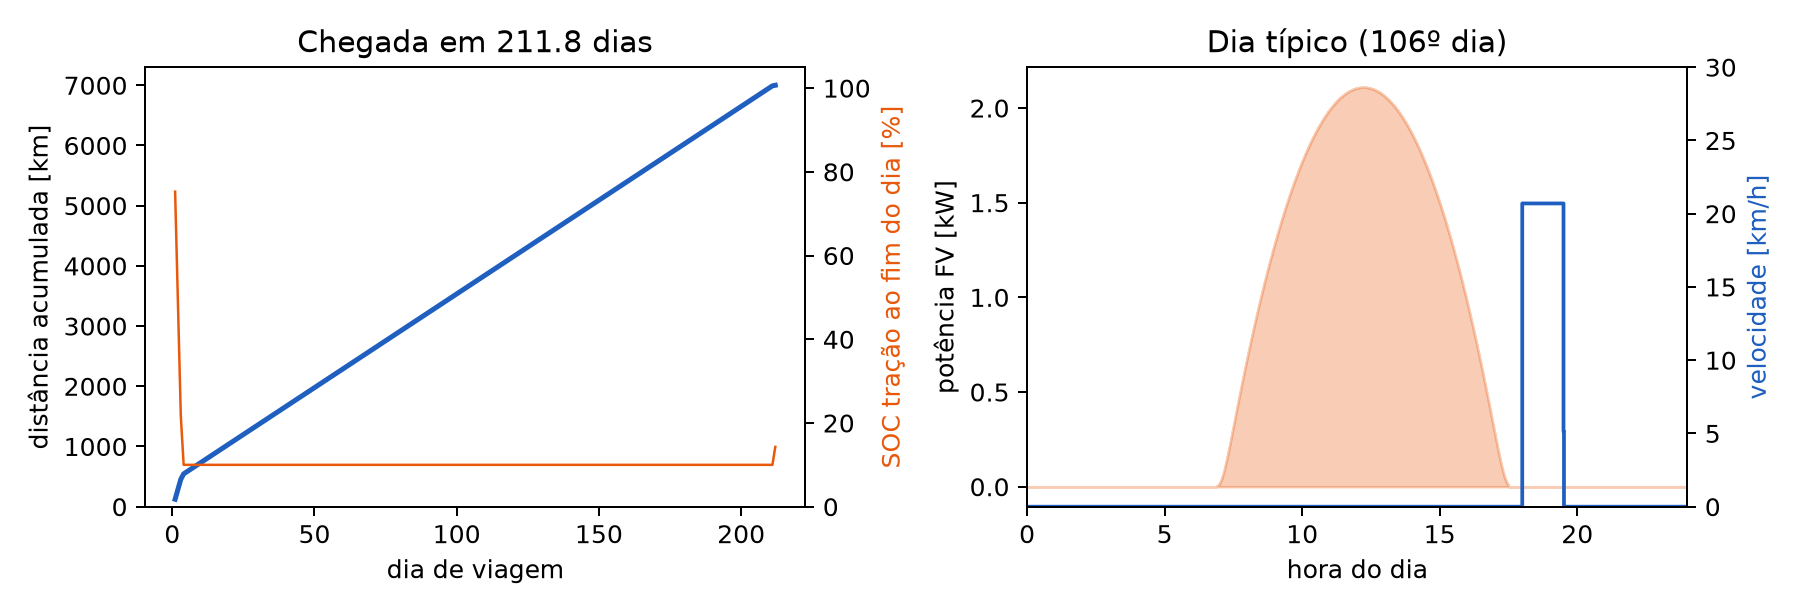
\includegraphics[width=\linewidth]{i29_missao.png}
\caption{Item 29 — distância acumulada e SOC da tração ao longo da viagem, e um dia típico.}\end{figure}}
\newcommand{\IbComparacao}{%
\begin{table}[H]\centering\small\setlength{\tabcolsep}{4pt}
\caption{Item 29 — mesma partida (18h00), mesmas reservas e mesma geração; só a velocidade muda.}
\label{tab:i29comparacao}
\begin{tabular}{rrrrrrr}
\toprule
$v$ & Viagem & Ao volante & Consumo & Até a reserva & \multicolumn{2}{c}{Depois da reserva} \\
{}[km/h] & [dias] & [h] & [kWh/km] & [km] & [km/dia] & [h/dia] \\
\midrule
20,5 & 214,8 & 341 & 0,198 & 539 & 30,6 & 1,49 \\
40,0 & 248,8 & 175 & 0,228 & 414 & 26,7 & 0,67 \\
80,0 & 457,8 & 88 & 0,408 & 216 & 14,8 & 0,19 \\
\bottomrule
\end{tabular}
\end{table}}
}{%
  \newcommand{\IbResposta}{\textbf{[pendente]}}\newcommand{\IbTexto}{}\newcommand{\IbResumo}{\textbf{[pendente]}}}

% Gerado por relatorio/atualizar_tabelas.py; cenário maxeon1560_independente.
\newcommand{\MassaNom}{4042,8}
\newcommand{\MargemNom}{207,2}
\newcommand{\CgX}{2,042}
\newcommand{\CgY}{-0,001}
\newcommand{\CgZ}{0,942}
\newcommand{\EixoDianteiro}{1997}
\newcommand{\EixoTraseiro}{2046}
\newcommand{\RolamentoNom}{476}
\newcommand{\MassaComChapas}{4075,9}
\newcommand{\MargemComChapas}{174,1}
\newcommand{\ConsumoQuarenta}{0,228}
\newcommand{\DistanciaEnergiaQuarenta}{4,39}
\newcommand{\PotenciaBateriaQuarenta}{9,10}
\newcommand{\ConsumoOitenta}{0,408}
\newcommand{\DistanciaEnergiaOitenta}{2,45}
\newcommand{\PotenciaBateriaOitenta}{32,68}
\newcommand{\AlcanceOitentaSoc}{248,0}
\newcommand{\AlcanceDia}{347,2}
\newcommand{\VelocidadeDia}{20,7}
\newcommand{\HorasDia}{16,8}
\newcommand{\PotenciaBatDia}{4,09}
\newcommand{\PotenciaRodaDia}{3,05}
\newcommand{\PotenciaMotorDia}{3,14}
\newcommand{\AlcanceOito}{307,2}
\newcommand{\VelocidadeOito}{38,4}
\newcommand{\HorasOito}{8,0}
\newcommand{\PotenciaBatOito}{8,57}
\newcommand{\PotenciaRodaOito}{7,09}
\newcommand{\PotenciaMotorOito}{7,31}
\newcommand{\AcelNoventa}{10,8}
\newcommand{\AcelCem}{12,7}
\newcommand{\AcelRaioNoventa}{10,58}
\newcommand{\AcelRaioCem}{12,49}
\newcommand{\AcelMinNoventa}{9,4}
\newcommand{\AcelMaxNoventa}{14,2}
\newcommand{\AcelMinCem}{11,3}
\newcommand{\AcelMaxCem}{16,3}
\newcommand{\FreioPico}{297,82}
\newcommand{\FreioRegenQuarenta}{256,98}
\newcommand{\FreioRegenOitenta}{217,34}
\newcommand{\MassaExtraCama}{66,3}
\newcommand{\MassaCamaInventario}{116,3}
\newcommand{\UtilCama}{0,833}
\newcommand{\FrenteMinAmbos}{1744}
\newcommand{\FrenteMaxAmbos}{2243}
\newcommand{\FrenteMinA}{1744}
\newcommand{\FrenteMaxA}{2234}
\newcommand{\TrasMinAmbos}{1693}
\newcommand{\TrasMaxAmbos}{2363}
\newcommand{\TrasMinA}{1744}
\newcommand{\TrasMaxA}{2363}
\newcommand{\MargemMinAmbos}{84}
\newcommand{\MargemMaxAmbos}{371}
\newcommand{\MargemMinA}{84}
\newcommand{\MargemMaxA}{331}
\newcommand{\AutSolarSemQuarenta}{56,3}
\newcommand{\AutSolarSemOitenta}{31,3}
\newcommand{\AutSolarComQuarenta}{27,2}
\newcommand{\AutSolarComOitenta}{15,2}
\newcommand{\AutSolarMax}{64,4}
\newcommand{\AutSolarVel}{21}
\newcommand{\SemDeckConsQuarenta}{0,221}
\newcommand{\SemDeckBatQuarenta}{8,83}
\newcommand{\DeckPercentualQuarenta}{3,0}
\newcommand{\DeckKmEmpateQuarenta}{884}
\newcommand{\SemDeckConsOitenta}{0,382}
\newcommand{\SemDeckBatOitenta}{30,53}
\newcommand{\DeckPercentualOitenta}{7,0}
\newcommand{\DeckKmEmpateOitenta}{221}


\begin{document}

\hypersetup{pageanchor=false}
\begin{titlepage}
\centering
{\large Universidade de São Paulo\par Escola de Engenharia de São Carlos\par}
\vspace{1.8cm}
{\Large SEM0571 — Sistemas Térmicos e Fluídicos\par}
\vspace{0.4cm}
{\LARGE\bfseries Projeto de um Motorhome Elétrico Solar\par}
\vspace{0.3cm}
{\Large Aurora Solar\par}
\vspace{1.5cm}
% Nomes fornecidos pelo usuário em 25/11/2026; manter esta grafia até nova orientação.
\begin{tabular}{l}
Matheus Hipolito\\
Matheus Alonso\\
Eduardo Barros Guimarães\\
Sabrina\\
Amanda\\
Vitor Dutra\\
Martinez\\
Henrick
\end{tabular}
\par
\vspace{1cm}
{Professores:\par Dr. Cristiano Bigonha Tibiriçá\par Dr. Paulo Seleghim Junior\par}
\vfill
{São Carlos\par Dezembro de 2026\par}
\end{titlepage}
\hypersetup{pageanchor=true}

{\small\tableofcontents}
\clearpage

%======================================================================
\section{Introdução}
O presente relatório tem como objetivo desenvolver e analisar o comportamento térmico,
energético e aerodinâmico de um veículo elétrico solar projetado especificamente para a
disciplina de Sistemas Térmicos e Fluídicos. O estudo segue as condições ambientais
definidas no enunciado, que correspondem a um dia de céu limpo em 21 de junho, na cidade
de São Carlos, com temperatura ambiente de 25 °C, umidade relativa de 50\% e ausência de
vento. Essas condições servem como base para avaliar tanto o desempenho quanto as
limitações do sistema.\footnote{A introdução e partes da fundamentação retomam a redação de Baratto et al.
\cite{cuca}, adaptada ao motorhome e às condições deste projeto.}

O trabalho envolve a definição completa do veículo, incluindo rodas, pneus, freios,
suspensão, motor, transmissão, baterias, controladoras e área de painéis fotovoltaicos.
A partir dessas especificações, são desenvolvidos modelos para estimar massas,
coeficientes aerodinâmicos, resistências térmicas e curvas de operação do motor elétrico.
Com esses modelos, o comportamento do motorhome é simulado considerando geração solar,
consumo energético e dissipação de calor nos componentes internos.

O projeto, denominado Aurora Solar, utiliza um Fiat E-Ducato L3H2 para duas pessoas,
com \SI{1560}{Wp} no teto e quatro painéis portáteis de \SI{400}{W}. A bateria de tração
é independente do banco de serviços. Nos problemas de autonomia solar, admite-se uma
interface externa de recarga CC, ainda não demonstrada fisicamente.

\subsection{Objetivos}
O projeto busca definir o veículo e seus componentes, calcular massa, resistências ao
movimento e capacidade energética, e avaliar seu desempenho nas condições do enunciado.
Para isso, são estudados o aquecimento dos freios, dos cabos, da bateria e da cabine,
bem como a capacidade dos sistemas de resfriamento.

A partir desses resultados, avaliam-se consumo, autonomia e alcance diário. A estratégia
de viagem procura percorrer \SI{7000}{km} no menor tempo nas condições testadas,
com até oito horas diárias de condução e sem energia da rede.

\clearpage
\section{Revisão Bibliográfica}
O desenvolvimento de veículos solares envolve a integração de tecnologias de diversas
áreas da engenharia, com foco principal em eficiência energética, desempenho aerodinâmico
e gestão térmica. A seguir, são apresentadas algumas das principais tecnologias e métodos
que possibilitam o desenvolvimento de carros solares \cite{cuca}.

\subsection{Tecnologias de Rodagem e Resistência ao Movimento}
A eficiência de um carro solar depende criticamente da redução de perdas mecânicas.
Entre elas, a resistência ao rolamento é uma das mais relevantes. Ela resulta sobretudo
da energia dissipada na deformação dos pneus e depende da pressão, carga e pista.
O arrasto aerodinâmico cresce com o quadrado da velocidade \cite{gillespie,hucho}.

\subsection{Motores Elétricos e Sistemas de Propulsão}
Motores elétricos brushless de alta eficiência são amplamente estudados para aplicação
em veículos solares devido ao seu elevado rendimento, baixa massa e grande confiabilidade.
A potência mecânica é dada por $P=T\omega$, em que $T$ é o torque e $\omega$ a
velocidade angular. Essa relação permite construir o envelope de potência a partir
da curva de torque e relacionar a rotação do motor à velocidade do veículo.
No E-Ducato, o motor síncrono de ímãs permanentes aciona as rodas dianteiras por um
redutor de relação fixa \cite{fiatsk,fiatde}.

\subsection{Armazenamento de Energia com Baterias de Íons de Lítio}
Para garantir segurança e longevidade, a literatura destaca o papel do Sistema de
Gerenciamento de Bateria (BMS), responsável por equalizar células, monitorar temperatura
e corrente e prevenir sobrecarga e descarga excessiva. O projeto utiliza baterias de fosfato de ferro-lítio (LFP):
a original para tração e módulos independentes para a habitação \cite{fiatsk,pylontech}.

\subsection{Conversão Fotovoltaica e Controladores MPPT}
Como a potência disponível depende da irradiância e da temperatura da célula, os
controladores com rastreamento do ponto de máxima potência (MPPT) são indispensáveis. Eles ajustam
dinamicamente o ponto de operação elétrico das células. O inversor converte a tensão
contínua (CC) do banco de serviços em tensão alternada (CA) para os aparelhos. A energia útil
depende também das perdas de conversão e do horário em que os painéis ficam expostos
ao sol \cite{maxeon,victron}.

\subsection{Uso de CFD e Simulações Térmicas}
A Dinâmica dos Fluidos Computacional (CFD) é uma ferramenta numérica utilizada para
modelar o comportamento do escoamento de ar ao redor de geometrias complexas,
permitindo prever grandezas aerodinâmicas sem a necessidade de ensaios físicos.
O escoamento e a condução são resolvidos por volumes finitos; balanços de energia
representam os demais sistemas. No arrefecimento, a bomba estabelece a vazão e o
radiador transfere calor ao ar, conforme as vazões e a condutância térmica $UA$.
Malha, passo temporal e conservação verificam as soluções numéricas
\cite{celik,incropera,apostila}.

\clearpage
\section{Projeto técnico}
\subsection{Especificações}
Considerando que o objetivo do motorhome é conciliar deslocamento e habitação,
as escolhas buscam reduzir massa e consumo, preservando os componentes originais
do fabricante (OEM).
Dessa forma, seguem os detalhes e componentes escolhidos para o projeto:
\begin{table}[htbp]\centering\small
\caption{Principais escolhas de projeto.}\label{tab:escolhas}
\begin{tabularx}{\linewidth}{lXX}
\toprule Sistema & Escolha / alternativa & Critério \\\midrule
Base & E-Ducato / construção própria & trem de força OEM e PBT de 4250 kg \\
Teto & 1560 / 1540 Wp & +20 Wp com a mesma massa e área \\
MPPT & dois / compartilhado & evitar descasamento do teto e portáteis \\
Serviços & três / dois, quatro ou cinco US5000 & 33 h sem sol com menor massa \\
Layout & cama fixa / conversível & acesso à lavadora e massas baixas \\
Climatização & FreshWell + cortina / aparelho maior & atender à carga sem trocar o aparelho \\
\bottomrule\end{tabularx}\end{table}
\designsec{Veículo e conceito}
\itemmark{1}
O nome escolhido pela equipe foi \textbf{Aurora Solar}. O veículo-base é o Fiat
E-Ducato L3H2, variante SK MY25 505.GG1.2, com PBT de \SI{4250}{kg}, tração dianteira,
bateria de \SI{98}{kWh} úteis e motor de \SI{205}{kW} \cite{fiatsk}.
\begin{figure}[htbp]
\centering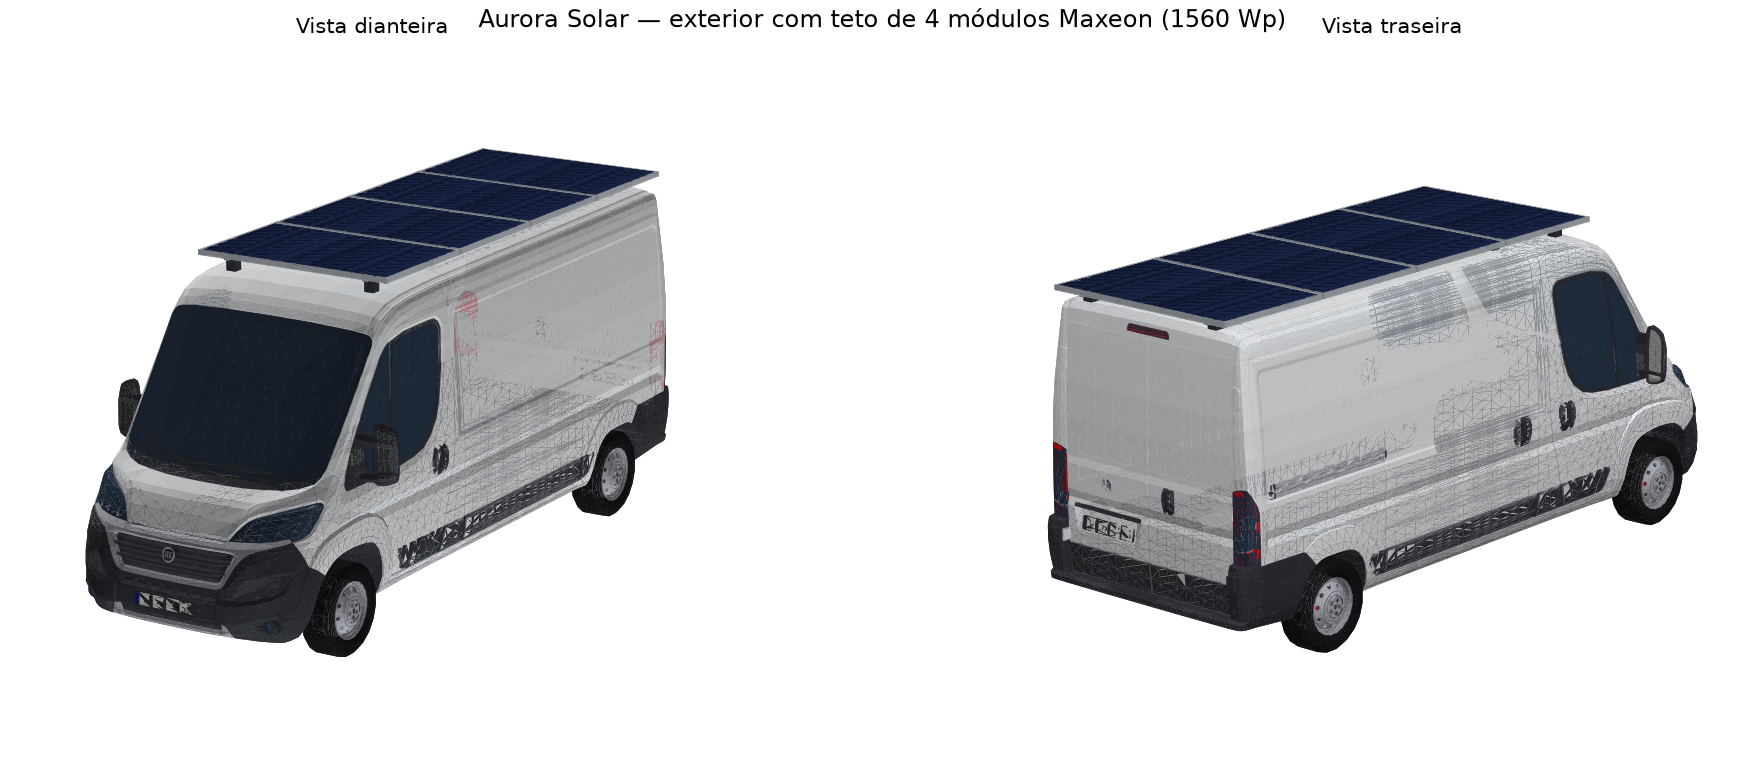
\includegraphics[width=0.85\linewidth]{cad_exterior.png}
\caption{Aurora Solar: Fiat E-Ducato L3H2 convertido, com o teto de quatro módulos Maxeon (1560 Wp). Renderização da geometria do projeto (carroceria derivada de razor24/Dogan Ulus, MPL-2.0 e CC-BY-4.0).}
\label{fig:exterior}
\end{figure}

\designsec{Pneus, rodas e freios}
\itemmark{2}
Foram adotados pneus \textbf{225/75 R16C 121R}, com o Continental VanContact A/S
04514690000 como referência (ficha norte-americana): diâmetro \SI{0,744}{m}, massa \SI{16,9}{kg} e capacidade
\SI{1449}{kg} por pneu \cite{conti}. São utilizadas quatro rodas de aço 6,5J$\times$16, além do estepe.

As pressões de referência são \SI{4,5}{bar} na dianteira e \SI{5,0}{bar} na traseira,
a confirmar na etiqueta da variante elétrica \cite{ducatomanual}. As cargas nominais
por pneu são aproximadamente 998 e \SI{1023}{kg}; isso não comprova os limites por eixo.
O estepe é considerado dentro da massa OEM, hipótese ainda a confirmar.

\itemmark{3}
São mantidos os freios hidráulicos a disco nas quatro rodas, ABS/ESC e regeneração OEM.
O disco dianteiro ventilado de \qtyproduct{300 x 32}{mm} usa o Brembo 09.D018.11 como
referência, sem confirmação por VIN dos discos, pinças e conjunto traseiro \cite{brembo}.

No modelo térmico adotam-se disco idealizado de \SI{5,1}{kg}, repartição dianteira/traseira
70/30 e propriedades de ferro fundido: $\rho=\SI{7100}{kg/m^3}$,
$c_p=\SI{500}{J/(kg.K)}$ e $k=\SI{51}{W/(m.K)}$ \cite{topczewska}.
A transferência de carga é calculada por $\Delta N=mah/L$; o aquecimento durante a frenagem é analisado na Seção~\ref{item:33}.

\designsec{Motor e transmissão}
\itemmark{4}
Motor síncrono de ímãs permanentes, 8 polos, \textbf{\SI{205}{kW} e \SI{410}{N.m}
de pico}. Torque constante até a rotação de base de \SI{4775}{rpm} e potência
constante acima dela (Figura~\ref{fig:motor}). Eficiência máxima de 95,5\,\% no modelo
de perdas; a \SI{90}{km/h} o motor gira a \SI{6608}{rpm} com redução 10:1.

\begin{figure}[htbp]
\centering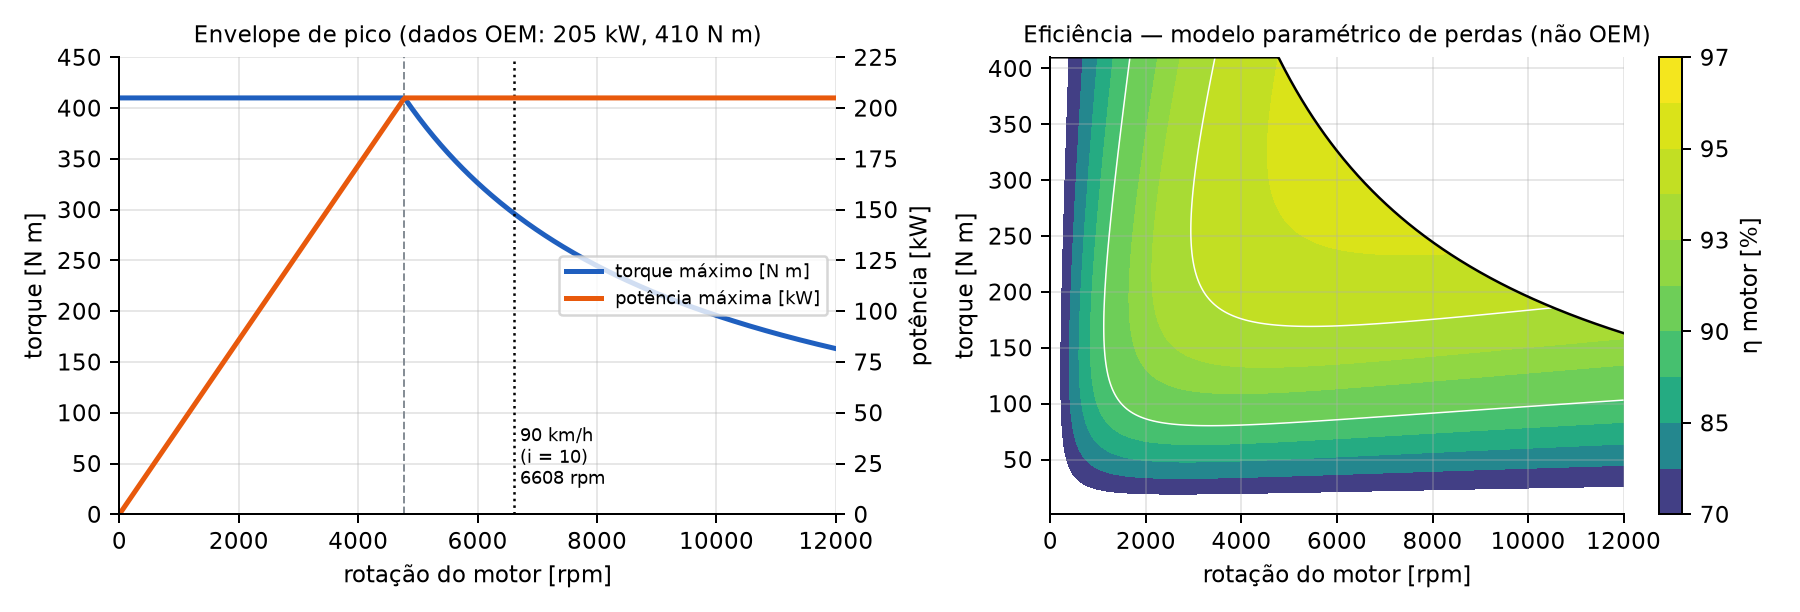
\includegraphics[width=\linewidth]{i04_motor.png}
\caption{Envelope de torque e potência a partir dos picos do fabricante, e mapa de
eficiência de um modelo de perdas calibrado com $\eta = 0{,}95$ no ponto de canto.}
\label{fig:motor}
\end{figure}

O mapa de eficiência usa perdas no cobre proporcionais a $T^2$, no ferro a
$\omega^{1,5}$, mecânicas a $\omega$ e uma parcela constante, divididas em
60/25/10/5\,\% no ponto de canto (\SI{410}{N.m}, \SI{500}{rad/s}):
\begin{equation}
\eta(T,\omega) = \frac{T\omega}{T\omega + k_c T^2 + k_i \omega^{1,5} + k_m \omega + P_0}.
\end{equation}
\limite{o fabricante publica só os picos; a forma do mapa é modelo, não medição.}

\itemmark{5}
O motor utiliza redutor de relação fixa com diferencial e tração dianteira \cite{fiatde}.
Como a relação numérica não é publicada, adota-se $i=10$ (sensibilidade 8--12) e rendimento
$\eta_{red}=0{,}97$ (0,95--0,99). São hipóteses, não especificações OEM.
Na potência máxima, as perdas calculadas no redutor são de \SIrange{2,1}{10,3}{kW}.

\designsec{Baterias e capacidade energética}
\itemmark{6}
A bateria de tração original utiliza a tecnologia LFP, com \SI{110}{kWh} brutos / \SI{98}{kWh} úteis,
\SI{400}{V}, 15 módulos, refrigeração líquida. O banco de serviços é formado por três módulos Pylontech US5000
(LFP, \SI{48}{V}, \SI{100}{Ah}, \SI{4,8}{kWh} cada, \SI{39,7}{kg},
\qtyproduct{442 x 420 x 161}{mm}), total \SI{14,4}{kWh} e \SI{119,1}{kg}, sob a cama.

O banco de serviços foi dimensionado para 24 a 48\,h de habitação sem sol. O estado
de carga (SOC) expressa a fração de energia disponível. Partindo de SOC 100\,\% e
parando em 30\,\% (reserva), três módulos dão $0{,}70 \times \SI{14,4}{kWh} = \SI{10,1}{kWh}$
utilizáveis; com a carga média de \SI{0,301}{kW} (\SI{7,23}{kWh/dia} retirados do banco, Tabela~\ref{tab:cargas}
do item 13), a habitação dura $10{,}1/0{,}301 \approx \SI{33}{h}$ sem geração.

\begin{figure}[htbp]
\centering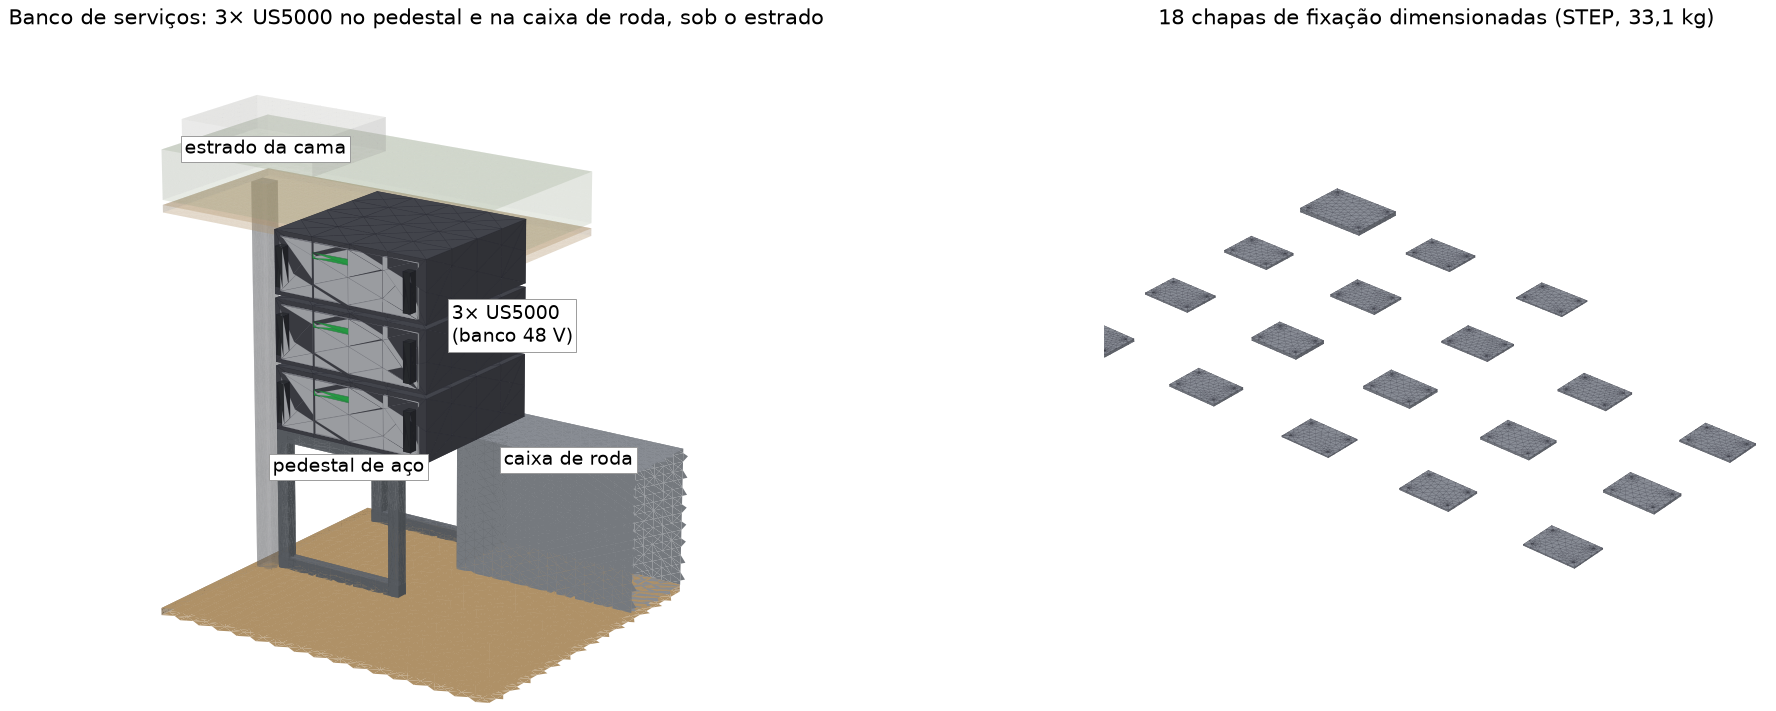
\includegraphics[width=\linewidth]{cad_banco_fixacoes.png}
\caption{Banco de serviços com três módulos US5000 sob o estrado da cama, no pedestal de aço e sobre a caixa de roda (montagem do layout A), e as 18 chapas de fixação da conversão (modelo STEP).}
\label{fig:banco}
\end{figure}

\itemmark{23}
Para comparar as capacidades, é preciso distinguir energia nominal e utilizável.
A soma de 112,4 kWh combina os 98 kWh úteis da tração com os 14,4 kWh nominais
dos serviços. Destes, cerca de 13,7 kWh são utilizáveis pela ficha, a 95\% de descarga
\cite{pylontech}; o total utilizável a bordo é, portanto, aproximadamente 111,7 kWh.

O SOC da tração usa a base útil de 98 kWh; o dos serviços usa 14,4 kWh nominais.
O item 27 reserva 30\% da tração; o item 29 usa reservas tração/serviços de 10/20 ou
20/30\%, mais restritivas que a profundidade máxima dos módulos de serviços.

\designsec{Geração fotovoltaica}
\itemmark{8}
O teto recebe quatro \textbf{Maxeon SPR-MAX3-390-COM}, em 2S2P: \SI{1560}{Wp},
\SI{76}{kg}, \SI{7,07}{m^2} e eficiência de 22,1\% \cite{maxeon}.
São acrescentados quatro EcoFlow de \SI{400}{W}, \SI{21}{kg} cada com bolsa, abertos apenas
com o veículo parado. Para separar o efeito dos portáteis do horário de uso, a Tabela~\ref{tab:i08casos}
e a Figura~\ref{fig:i08} comparam quatro condições no mesmo dia claro.

Em 2S2P, $V_{mp}=2(64{,}5)=\SI{129}{V}$ e $I_{mp}=2(6{,}05)=\SI{12,10}{A}$.
O $V_{oc}$ a \SI{-20}{\celsius}, com tolerância, é \SI{171,59}{V}; a saída ideal a 48 V
é \SI{32,5}{A}, dentro do MPPT 250/60. Quatro módulos em paralelo cairiam a cerca de
\SI{49}{V} a \SI{85}{\celsius}, sem margem para carregar a \SI{53,2}{V}.
A troca de 1540 por 1560 Wp mantém massa e dimensões e acrescenta \SI{0,076}{kWh/dia}.
\begin{table}[htbp]
\centering\small
\caption{Geração em 21/06 por caso de operação (São Carlos, céu limpo).}
\label{tab:i08casos}
\begin{tabular}{lrrr}
\toprule
Caso & Teto [kWh] & Portáteis [kWh] & Total [kWh] \\
\midrule
Só teto & 5,94 & 0 & 5,94 \\
Parado o dia todo, portáteis prontos antes do amanhecer & 5,94 & 8,55 & 14,49 \\
Condução diurna, 08--16\,h & 5,94 & 0,37 & 6,31 \\
Condução no fim da tarde, 18--02\,h & 5,94 & 8,55 & 14,49 \\
\bottomrule
\end{tabular}
\end{table}
\begin{figure}[htbp]
\centering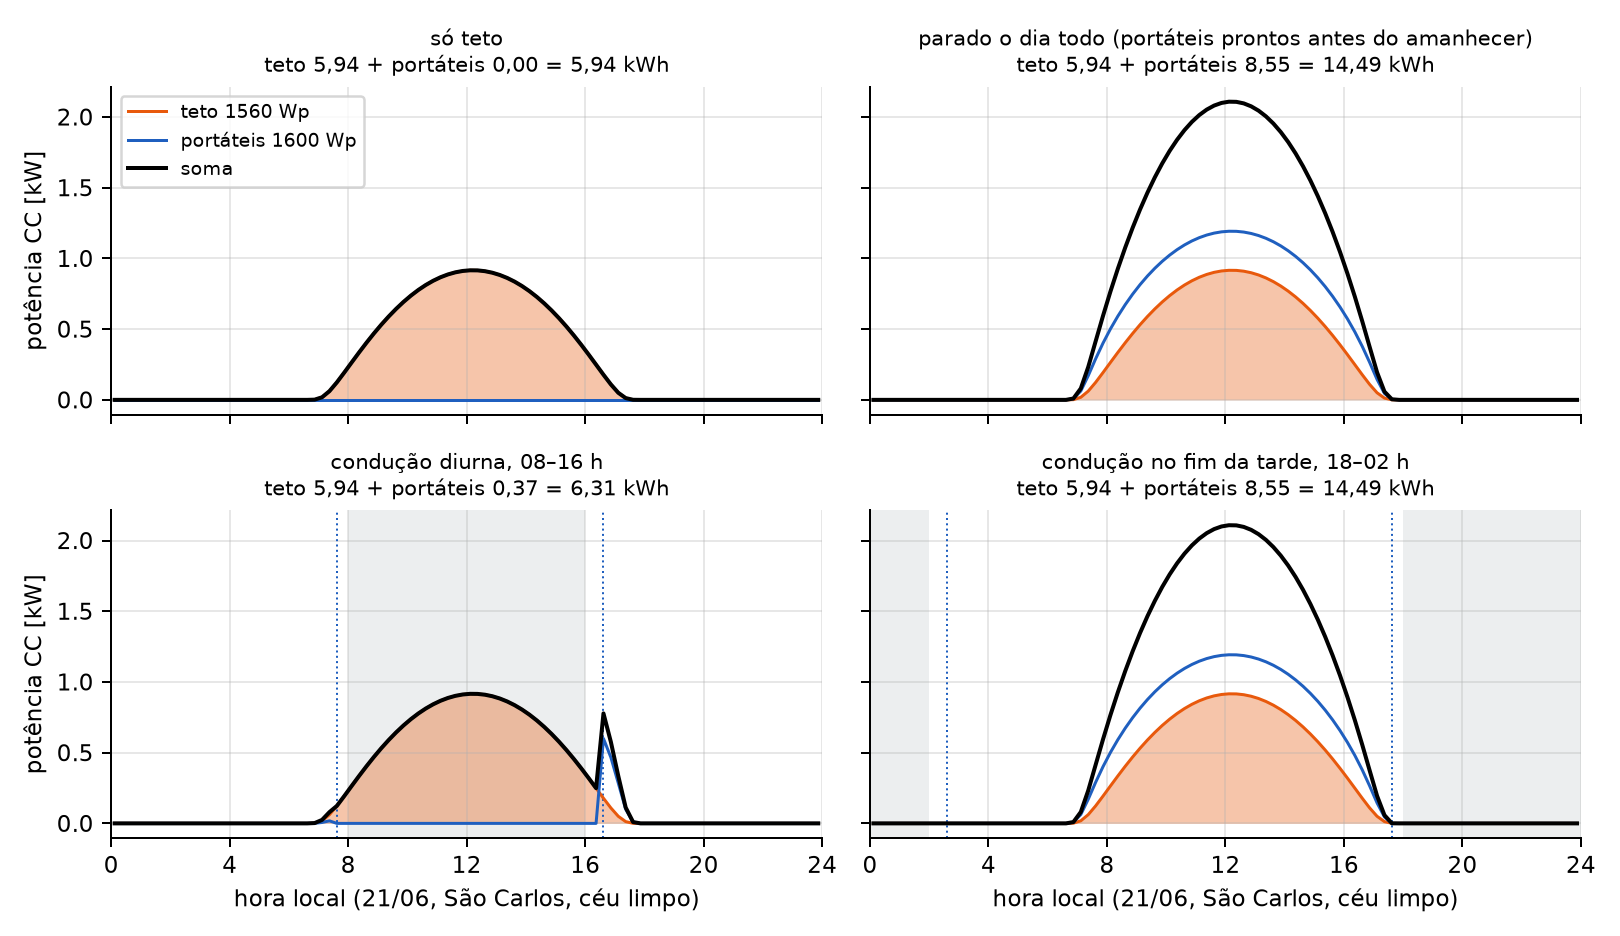
\includegraphics[width=\linewidth]{i08_geracao_solar.png}
\caption{Potência CC do teto, dos portáteis e soma em 21/06 (pvlib, céu claro, modelo térmico
de Faiman, 10\,\% de perdas) nos quatro casos. Faixa cinza: condução; linhas pontilhadas: fim da
montagem e início do recolhimento dos portáteis.}
\label{fig:i08}
\end{figure}

Os portáteis ficam a \ang{45}, voltados para o norte. Adotam-se 30 min para montar e
30 min para recolher, hipótese comum às marcas. A tabela considera quatro unidades.
\begin{table}[htbp]
\centering\small
\setlength{\tabcolsep}{3pt}
\caption{Painéis portáteis, quatro unidades (fichas consultadas em 25/11/2026; nenhum ensaiado).}
\label{tab:portateis}
\begin{tabular}{lcccc}
\toprule
 & EcoFlow 400 (atual) & EcoFlow 400 Lightweight & ZOUPW 450 & Renogy RSP400LSC \\
\midrule
Potência [Wp] & 1600 & 1600 & 1800 & 1600 \\
Energia por parada [kWh] & 8,55 & 8,55 & 9,62 & 8,58 \\
Massa [kg] & 84 (com bolsa) & 40,8 & 48,6 & 54,8 \\
Aberto, cada [m] & $2,39\times1,07$ & $2,51\times0,97$ & $3,10\times0,88$ & $2,84\times0,86$ \\
Dobrado, cada [m] & $1,07\times0,60\times0,07$ & $0,97\times0,66\times0,04$ & $0,88\times0,77\times0,09$ & $0,86\times0,71\times0,08$ \\
$V_{oc}$ 2S a \SI{-20}{\celsius} [V] & 110 & 90 & 105 & 106 \\
Preço unitário & R\$ 5.712 & EUR 649 & USD 460 & USD 495,99 \\
\bottomrule
\end{tabular}
\end{table}

Como as massas publicadas das alternativas não incluem acessórios, adota-se
\SI{1}{kg} adicional por unidade. Com isso, os conjuntos Lightweight, ZOUPW e Renogy
pesam, respectivamente, 44,8, 52,6 e 58,8 kg. As fichas são específicas do
EcoFlow Lightweight, ZOUPW 450 W N-Type 16BB e Renogy RSP400LSC-G1 \cite{ecoflowlw,zoupw,renogy}.
Não se confirmou equivalência deste último com o nome E.FLEX. A loja oficial indicava
USD 495,99/unidade, sem estoque em 25/11: USD 1.983,96 por quatro, sem frete/impostos
\cite{renogypreco}. O cenário principal mantém os EcoFlow atuais.

Os quatro candidatos atendem à verificação por ficha do MPPT 150/60 em 2S2P: $V_{oc}$ frio abaixo de 150 V e
$I_{sc}$ abaixo de 50 A. Os envelopes dobrados cabem no espaço de
\qtyproduct{1,10 x 0,38 x 0,98}{m}, com retirada pelas portas traseiras; conectores e
acessórios exigem conferência. Uma fileira leste--oeste ocupa 3,7--4,6 m por 1,7--2,2 m;
para duas fileiras, a distância contra sombra às 9h é 3,7--4,8 m.

A retenção dos \SI{84}{kg} usa $F=5mg=\SI{4,12}{kN}$: duas cintas independentes de pelo
menos \SI{5}{kN} cada e contenção positiva. A resistência dos olhais OEM não foi demonstrada.

Como sensibilidade, inclinar o teto para norte em 5/10/20° eleva sua energia de 5,94
para 6,43/6,89/7,65 kWh. A 20° para sul são 3,61 kWh; para leste/oeste a variação fica
abaixo de 0,24 kWh. O mecanismo não foi projetado; o uso seria estacionado.

A Figura~\ref{fig:inclinacao_comparada} separa os efeitos da inclinação e da orientação:
na mesma data, inclinar para o norte aumenta a captação, enquanto inclinar para o
sul a reduz. O ganho de 1,71 kWh/dia a 20° norte é potencial e não inclui massa,
custo, sombras ou esforço de um mecanismo de inclinação.
\begin{figure}[htbp]\centering
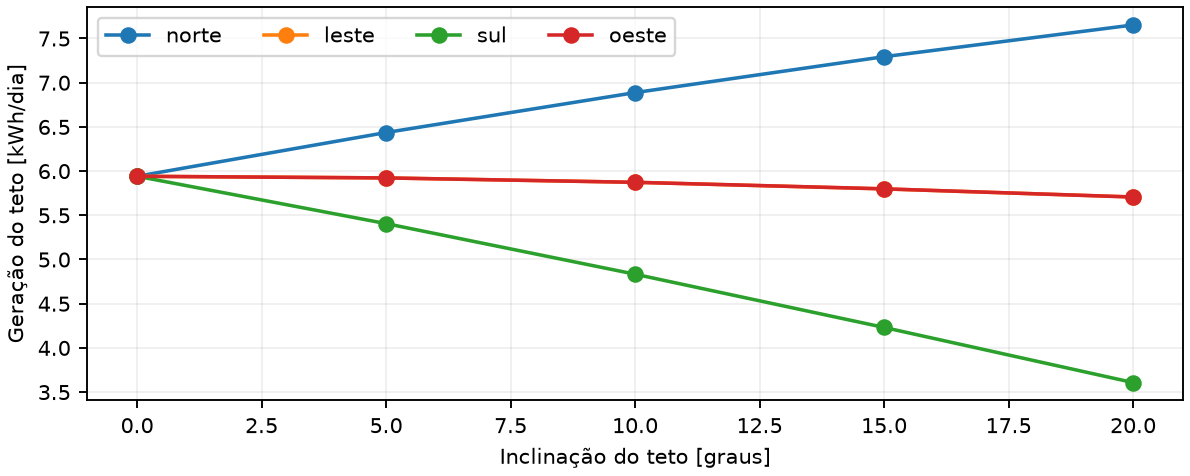
\includegraphics[width=0.75\linewidth]{comparacao_inclinacao.png}
\caption{Energia do mesmo teto ao variar inclinação e orientação, mantendo dia, clima e potência nominal.}
\label{fig:inclinacao_comparada}
\end{figure}

\begin{figure}[htbp]
\centering
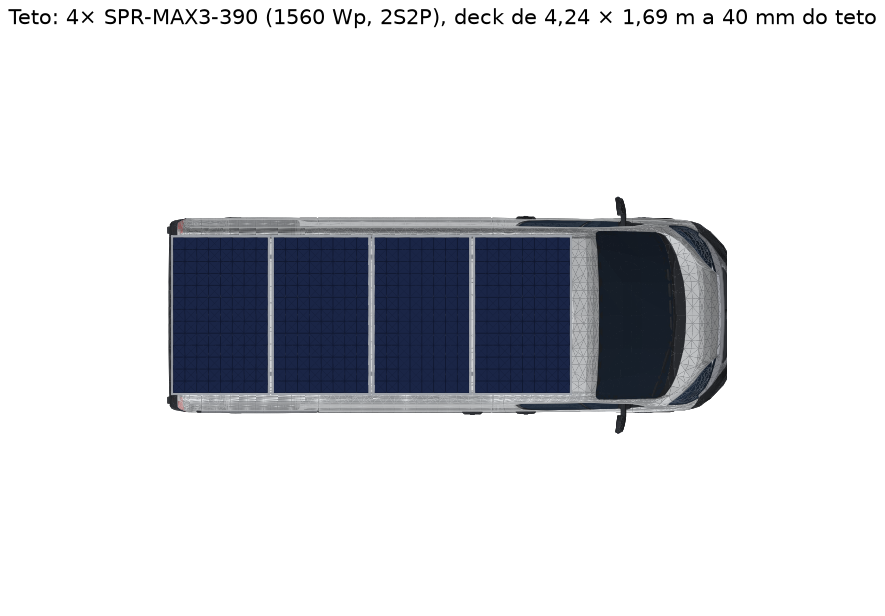
\includegraphics[width=0.49\linewidth]{cad_teto.png}\hfill
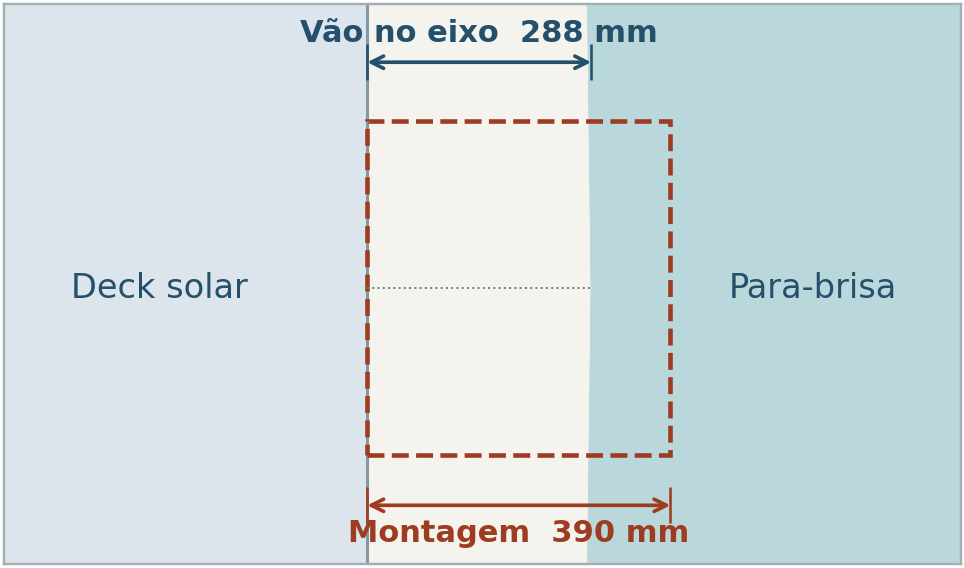
\includegraphics[width=0.50\linewidth]{i16_folga.png}
\caption{Teto com quatro painéis (4 SPR-MAX3-390) no deck de \qtyproduct{4,24 x 1,69}{m}. No detalhe, a faixa central até o para-brisa mede \SI{288}{mm}. O gabarito de instalação da Micro Heki exige pelo menos \SI{390}{mm} nessa direção.}
\label{fig:teto}
\end{figure}
\begin{figure}[htbp]
\centering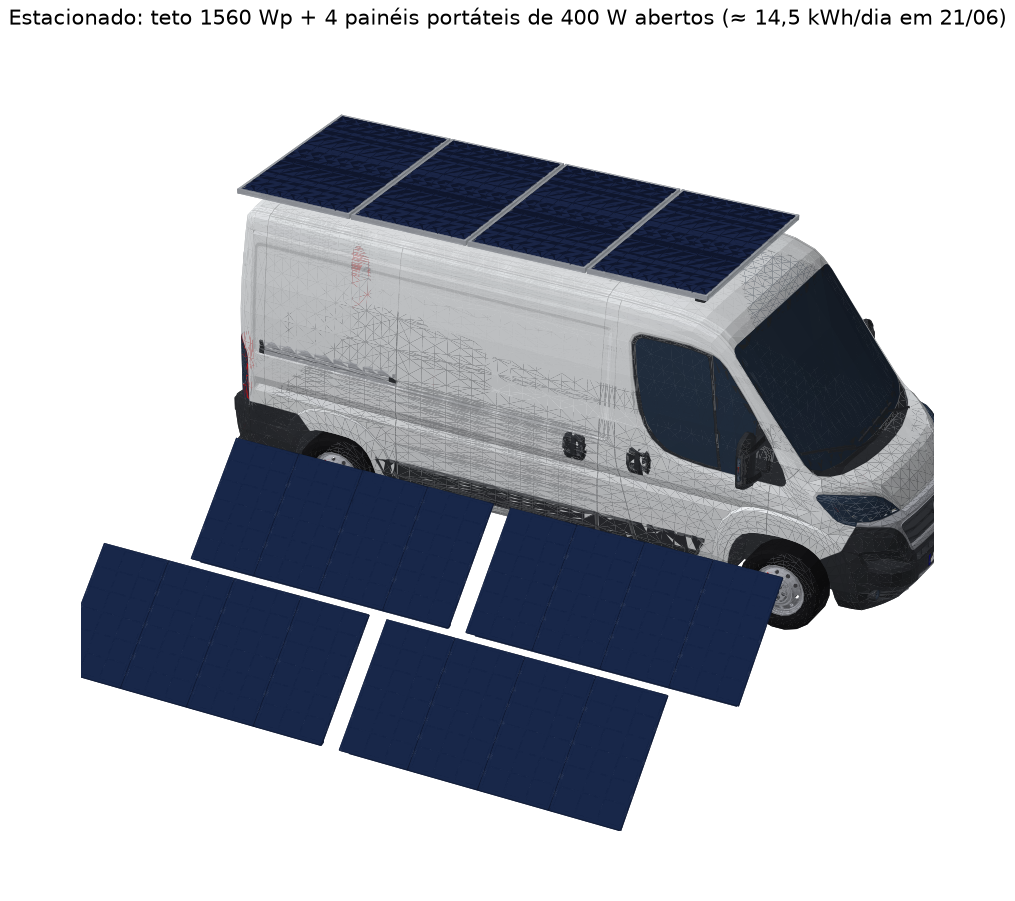
\includegraphics[width=0.8\linewidth]{cad_estacionado.png}
\caption{Configuração estacionada: teto e quatro painéis portáteis de \SI{400}{W} abertos no solo, voltados para o norte a \ang{45}.}
\label{fig:estacionado}
\end{figure}

\designsec{Instalação elétrica e conversores}
\itemmark{7}
A instalação de serviços utiliza cobre de \SIrange{70}{120}{mm^2} a \SI{48}{V},
fusível JLLN 200 A/20 kA e JLLN 80 A no MPPT. Os aparelhos recebem \SI{220}{V}/\SI{60}{Hz};
iluminação e bombas usam conversor de \SI{12}{V}. O chicote de alta tensão permanece OEM;
a capacidade térmica da referência RADOX de \SI{120}{mm^2} é avaliada na Seção~\ref{item:30} \cite{radox}.

Em 324 casos, a corrente de operação chega a \SI{103}{A} e a queda de tensão a 0,74\%.
Nos 144 casos de falta, com resistência interna de \SIrange{10}{40}{m\ohm} por módulo,
o envelope de \SIrange{2,75}{16,05}{kA} fica abaixo dos \SI{20}{kA} do fusível.
O limite publicado do US5000, $<\SI{2000}{A}/\SI{1}{ms}$ por módulo, reduz 63 casos \cite{pylontech}.
A varredura de referência de \SIrange{1}{50}{m\ohm}, mais ampla, produz 56 casos
acima de 20 kA antes da atuação do BMS; a conclusão depende, portanto, da resistência real dos módulos. A capacidade
de condução de corrente na instalação e a coordenação das curvas I²t ainda precisam
ser verificadas.
\begin{figure}[htbp]
\centering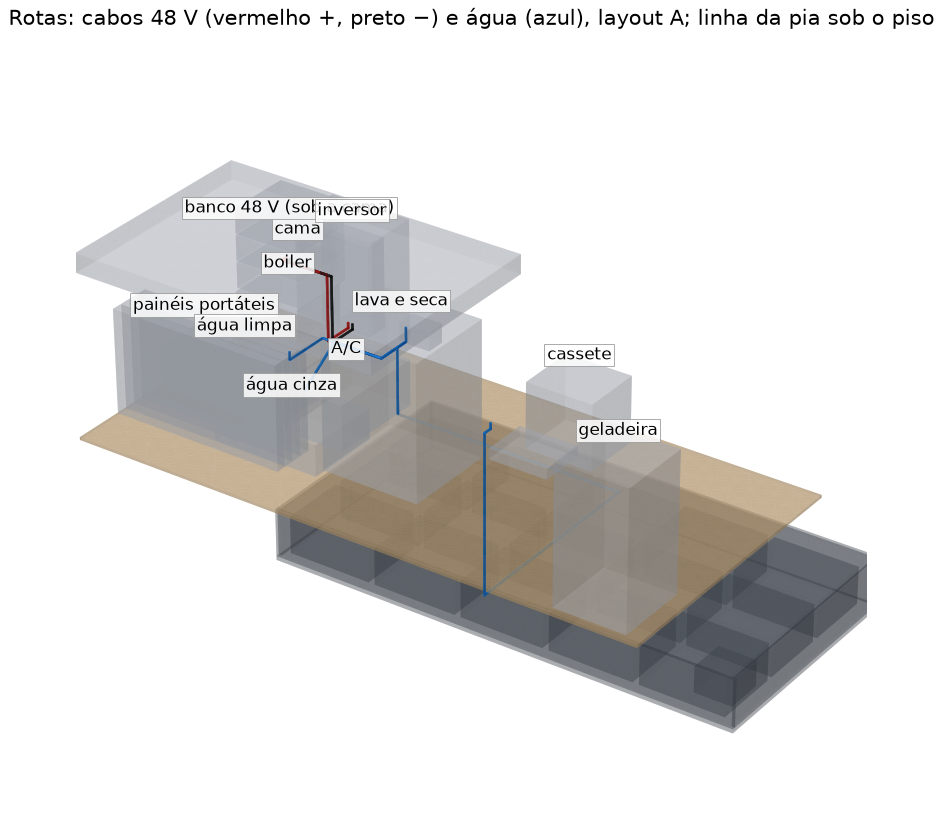
\includegraphics[width=0.85\linewidth]{cad_rotas.png}
\caption{Rotas reservadas de cabos de \SI{48}{V} (positivo em vermelho, retorno em preto) e de água (azul) no layout A; equipamentos em cinza translúcido. A linha da pia corre sob o piso e sobe atrás do gabinete da cozinha.}
\label{fig:rotas}
\end{figure}

\itemmark{9}
Foram escolhidos dois MPPT independentes: \textbf{SmartSolar 250/60-Tr} no teto e
\textbf{150/60-Tr} nos portáteis. Separá-los evita o descasamento de curvas I--V,
que causou perdas de 0,7--27\% em 72 casos de rastreador compartilhado.

Os picos de eficiência dos MPPT são 99\% (250/60) e 98\% (150/60).
Cada controlador Tr mede 185×250×95 mm e tem 3 kg \cite{victronmpptdim}.

O inversor é o \textbf{MultiPlus-II GX 48/5000/70-50}: \SI{4000}{W} contínuos a
\SI{25}{\celsius}, pico de eficiência 96\%, vazio de \SI{18}{W} e massa de \SI{31}{kg}
\cite{victron}. Seu envelope é 323×148×565 mm. Ele é dimensionado pela simultaneidade das cargas CA; acrescentar
20 Wp no teto não muda essa escolha.

No balanço, as perdas FV são 10\%; os rendimentos agregados do inversor e do conversor
CC são 0,90. Os bancos são distintos: a tração só recebe solar por uma interface externa
CCS2 hipotética, com o veículo parado, $\eta_{CC}=0{,}90$ e mínimo de
\SI{0,38}{kW} na saída. O modelo aloca geração fotovoltaica a essa interface;
não transfere a energia armazenada no banco de serviços para a tração.
\begin{figure}[htbp]
\centering
\begin{tikzpicture}[fluxo]
\node[caixa] (sol) at (0,0) {Sol};
\node[caixa] (teto) at (2.7,1.3) {teto\\1560\,Wp};
\node[caixa] (port) at (2.7,-1.3) {portáteis\\1600\,Wp (parado)};
\node[caixa] (m1) at (5.5,1.3) {MPPT\\250/60-Tr};
\node[caixa] (m2) at (5.5,-1.3) {MPPT\\150/60-Tr};
\node[caixa] (banco) at (9,1.3) {banco de serviços\\48\,V, 14,4\,kWh};
\node[caixa] (inv) at (12.5,1.3) {inversor\\MultiPlus-II};
\node[caixa] (ca) at (15,1.3) {cargas CA\\220\,V};
\node[caixa] (cc) at (12.5,-0.4) {CC-CC\\12\,V};
\node[hipo] (if) at (10,-3.5) {interface CC externa hipotética\\$\eta=0{,}90$; $P_{\text{saída}}\ge\SI{0,38}{kW}$};
\node[caixa] (hv) at (14.5,-3.5) {bateria de tração\\400\,V, 98\,kWh úteis};
\draw[seta] (sol) -- (teto); \draw[seta] (sol) -- (port);
\draw[seta] (teto) -- (m1); \draw[seta] (port) -- (m2);
\draw[seta] (m1) -- (banco); \draw[seta] (m2.east) -- (banco.south);
\draw[seta] (banco) -- (inv); \draw[seta] (inv) -- (ca); \draw[seta] (banco) -- (cc);
\coordinate (alocacao) at (6.8,-3.5);
\draw[dashed,thick] (6.8,1.3) -- (alocacao);
\draw[dashed,thick] (m2.east) -- (6.8,-1.3);
\node[font=\scriptsize,fill=white,inner sep=1pt,anchor=east] at (6.6,-2.3) {parcela FV alocada};
\draw[seta,dashed] (alocacao) -- (if.west);
\draw[seta,dashed] (if) -- (hv);
\end{tikzpicture}
\caption{Fluxos de energia nos estudos. Os rastreadores alimentam os serviços; o ramo tracejado
representa a alocação conceitual de parte da geração FV à recarga CC da tração. Não há
transferência da carga armazenada entre os bancos. O desenho não é um esquema de ligação elétrica.}
\label{fig:fluxo_eletrico}
\end{figure}
\begin{figure}[htbp]\centering
\begin{minipage}{0.44\linewidth}\centering
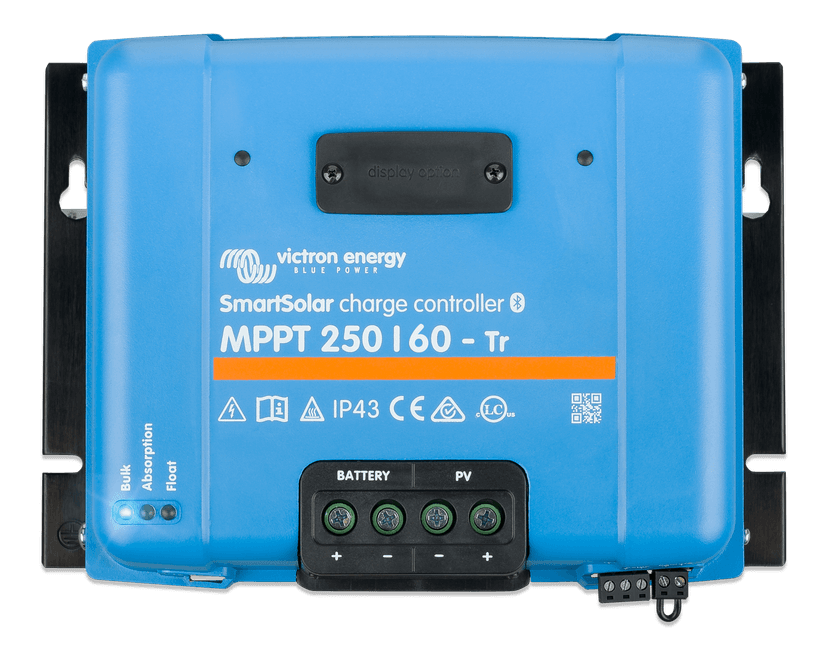
\includegraphics[height=5cm,width=\linewidth,keepaspectratio]{produtos/mppt.png}\par
\small SmartSolar MPPT 250/60-Tr
\end{minipage}\hfill
\begin{minipage}{0.44\linewidth}\centering
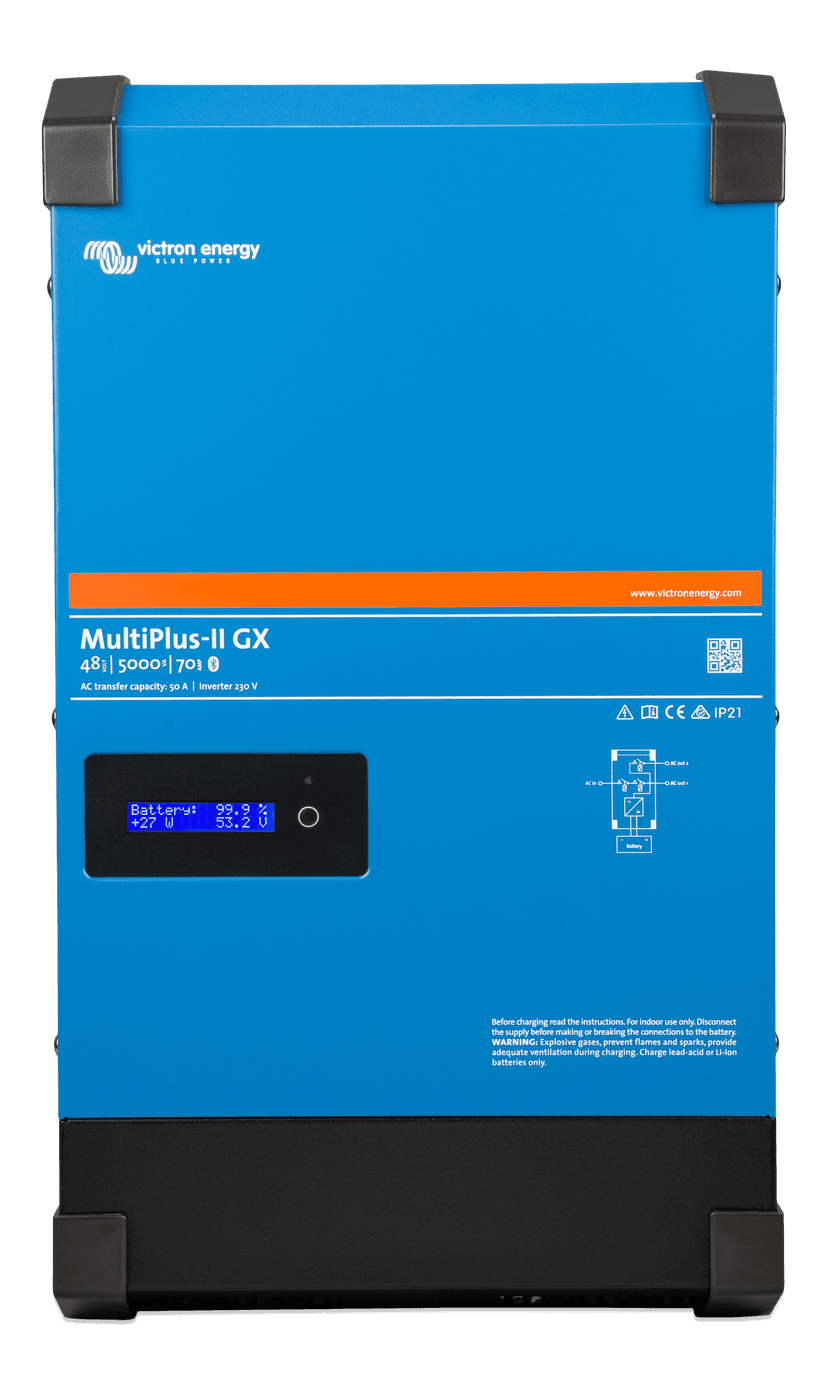
\includegraphics[height=5cm,width=\linewidth,keepaspectratio]{produtos/inversor.png}\par
\small MultiPlus-II GX 48 V / 5 kVA
\end{minipage}
\caption{Fotografias de catálogo dos equipamentos de conversão escolhidos. Fonte:
Victron Energy \cite{victronfotos}; as condições de eficiência e a configuração elétrica são as
indicadas no texto, e não inferidas da fotografia.}
\label{fig:produtos_eletricos}
\end{figure}

\designsec{Arrefecimento e lubrificação}
\itemmark{10}
Adota-se circuito líquido de água-glicol 50/50, radiador frontal, ventilador e bomba
elétrica, tendo a Bosch PCE2-XL 039202453G como referência \cite{bosch}.
Na potência de \SI{205}{kW}, o calor do motor/inversor, incluindo os \SI{96}{W} da bomba,
é 10,9/22,9/36,3 kW para rendimentos combinados de 95/90/85\%.
O caso de 90\% é conservador; o cálculo da bomba e do radiador é apresentado na Seção~\ref{item:35}.


\begin{table}[htbp]\centering\small
\caption{Componentes do circuito térmico. OEM significa mantido na tara do veículo.}
\label{tab:arrefecimento_especificacoes}
\begin{tabularx}{\linewidth}{lXr}
\toprule Componente / quantidade & Material, dimensão e origem & Massa \\\midrule
Bomba, 1 & Bosch PCE2-XL, 12 V; corpo de Ø77,2 mm, comprimento cotado de 109 mm, conexão Ø20 mm \cite{bosch} & 0,46 kg \\
Radiador, 1 & tubos e aletas de alumínio, hipótese; núcleo estimado 650×500×65 mm; $UA$ deve ser verificado & OEM \\
Ventilador, 1 & conjunto axial OEM; vazão de ar de 1 kg/s assumida; curva/dimensões não obtidas & OEM \\
Fluido & água/MEG 50/50; $\rho=1050$ kg/m³, $c_p=3500$ J/(kgK), $\mu=1{,}5$ mPa·s; volume OEM desconhecido & OEM \\
Mangueiras, 6 m & elastômero compatível, hipótese; diâmetro interno de 20 mm & OEM \\
Vaso/tampa, 1 & vaso polimérico; tampa de 100 kPa(g) é hipótese do estudo de NPSH & OEM \\
Bateria, 1 circuito & placa fria e resfriador equivalente; 20 kg de fluido na hipótese térmica; não é refrigerante do A/C & OEM \\
\bottomrule\end{tabularx}\end{table}

O armário de 48 V precisa rejeitar $4000(1/0{,}90-1)=444$ W.
Para elevar o ar em até 10 K, $\dot V=\dot Q/(\rho c_p\Delta T)\approx145$ m³/h.
O ventilador e seus dutos ainda não foram selecionados; massa/custo ficam nas reservas
de montagem/elétrica. O FreshWell da habitação é independente do circuito da bateria.

\itemmark{12}
O veículo não utiliza óleo de motor. Permanecem o óleo do redutor/diferencial,
as graxas dos rolamentos e articulações e o óleo do compressor do ar-condicionado.
O grau e o volume do óleo do redutor não foram publicados para a variante.

As perdas de \SIrange{2,1}{10,3}{kW} no redutor aquecem óleo e carcaça durante o pico.
Em regime, precisam seguir para o circuito líquido pela carcaça ou por trocador
óleo--água; a convecção natural isolada não basta.


\begin{table}[htbp]\centering\small
\caption{Lubrificantes típicos; confirmar cada produto e volume pelo VIN.}
\begin{tabularx}{\linewidth}{lXX}
\toprule Aplicação & Tipo de referência & Quantidade / massa \\\midrule
Redutor/diferencial & fluido de baixa viscosidade para VE, em banho & 1--2 L típicos; não é volume OEM confirmado \\
Rolamentos & graxa de complexo de lítio NLGI 2 & conjunto selado OEM, incluído na tara \\
Homocinéticas & graxa específica para juntas homocinéticas & carga selada OEM \\
Compressor elétrico & óleo POE dielétrico, referência típica & carga selada; quantidade OEM desconhecida \\
Direção EPS & assistência elétrica & sem fluido hidráulico \\\bottomrule
\end{tabularx}\end{table}
Para $\eta_m=0{,}95$, o motor/inversor tem perdas combinadas de 15,2--17,5 kW
com inversor a 98--97\%. A hipótese térmica conservadora de 90\% usa 22,9 kW.
O redutor a 95/97/99\% perde 10,25/6,15/2,05 kW no pico; sua ligação hidráulica
não foi identificada. O item 35 separa essa carga para evitar omiti-la ou contá-la duas vezes.

\designsec{Interior e climatização}
\itemmark{11}
\textbf{Dometic FreshWell 3000} sob o banco (\SI{2700}{W} de frio, até \SI{3000}{W} de
aquecimento, \SI{220}{V}, \SI{21}{kg}, \qtyproduct{626 x 400 x 286}{mm})
\cite{dometic}. A ventilação natural é feita pelas janelas, com apoio mecânico quando necessário. O arranjo de quatro painéis mantém o teto sem claraboia (Figura~\ref{fig:teto}).

O balanço de CO$_2$ em regime permanente (mistura perfeita) pede \SI{62}{m^3/h} de ar
externo para manter \SI{1000}{ppm} com duas pessoas; com \SI{30}{m^3/h}, o equilíbrio
seria \SI{1620}{ppm}. Os 648 casos de sensibilidade mostram ventiladores de
\SIrange{0,2}{17,5}{W}. A capacidade necessária para manter o conforto é avaliada na Seção~\ref{item:32}.

\itemmark{13}
\begin{table}[htbp]
\centering\small
\caption{Equipamentos e materiais internos (layout A, cama fixa).}
\begin{tabularx}{\linewidth}{lXr}
\toprule
Sistema & Marca/modelo e características & Massa [kg] \\
\midrule
Assentos & 2 bancos dianteiros do fabricante, giratórios para a área social & OEM \\
Cama & estrado de 30 mm, quadro 50×50×3, postes 45×45×4 e colchão de espuma & \MassaCamaInventario \\
Mobiliário & piso, tampo e divisórias em compensado naval & 82,2 \\
Isolamento & Armaflex AF de \SI{32}{mm} + revestimento de \SI{6}{mm} & 151,5 \\
Toalete/chuveiro & cassete Thetford Porta Potti 365 (\SI{21}{L}); box com chuveiro & 4,0 + 21,2 \\
Água & tanques \SI{100}{L} limpa / \SI{70}{L} cinza, bomba Shurflo 4008 \SI{12}{V}, boiler Quick B3 \SI{15}{L} \SI{500}{W} & 17,3 + água \\
Fogão & cooktop de indução Electrolux IE3TP, 1 zona, \SI{220}{V} & 2,3 \\
Geladeira & frigobar Midea MRC10B2, \SI{93}{L}, compressor, \SI{14,1}{kWh/\text{mês}} & 20,8 \\
Lavadora/secadora & LG lava e seca VC2, \SI{220}{V} & 73,0 \\
Eletrônicos & iluminação LED, carregadores USB, monitor de bateria (GX) & em cabos \\
Climatização & Dometic FreshWell 3000 (item 11) & 21,0 \\
\bottomrule
\end{tabularx}
\end{table}

O layout A utiliza cama fixa, cozinha e banheiro. O consumo de referência é de
\SI{60}{L/dia}, com reabastecimento e descarte diários; a lavadora usa \SI{68,8}{L/ciclo}.
\begin{table}[htbp]
\centering\small
\setlength{\tabcolsep}{4pt}
\caption{Consumo diário da habitação (duas pessoas, uso moderado; valores estimados).}
\label{tab:cargas}
\begin{tabular}{llllr}
\toprule
Aparelho & Alim. & Potência & Uso adotado & Energia [kWh/dia] \\
\midrule
Frigobar Midea MRC10B2 & CA & \SI{19,6}{W} médios & contínuo; ficha \SI{14,1}{kWh/\text{mês}} & 0,47 \\
Cooktop de indução IE3TP & CA & \SI{2000}{W} & cerca de 30\,min/dia & 1,00 \\
Ar-condicionado FreshWell & CA & \SI{1,15}{kW} elétricos (item 32) & 2,6\,h/dia na referência sem cortina & 3,00 \\
Boiler Quick B3 & CA & \SI{500}{W} & \SI{40}{L/dia} de 25 para \SI{38}{\celsius} & 0,72 \\
Lava e seca LG VC2, lavagem & CA & \SI{290}{W} médios/ciclo & 1 h/ciclo; 1 ciclo/semana & 0,04 \\
Lava e seca LG VC2, secagem & CA & \SI{1000}{W} médios/ciclo & 2 h/ciclo; 1 ciclo/semana & 0,29 \\
LED, eletrônicos e bombas & CC & \SI{75}{W} médios no uso & 8 h/dia distribuídas & 0,60 \\
\midrule
\multicolumn{4}{l}{Energia nos aparelhos (CA 5,52 + CC 0,60)} & 6,12 \\
\multicolumn{4}{l}{Perdas de conversão (inversor e conversor de \SI{12}{V}, rendimento 0,90)} & 0,68 \\
\multicolumn{4}{l}{Consumo em vazio do inversor (\SI{18}{W} $\times$ 24\,h)} & 0,43 \\
\midrule
\multicolumn{4}{l}{\textbf{Energia retirada do banco de serviços}} & \textbf{7,23} \\
\bottomrule
\end{tabular}
\end{table}

Consumo do frigobar, potência da indução e dados de lavagem/boiler vêm das fichas
\cite{midea,inducao,lavadora,boiler}. Tempos de uso, secagem e eletrônicos são hipóteses;
os ciclos semanais são rateados. O boiler usa $Q=mc_p\Delta T/\eta$, não 500 W durante 24 h.

Com perdas e vazio separados, o banco fornece \SI{7,23}{kWh/dia}, média de \SI{0,301}{kW}.
O perfil horário prevê refeições às 8h/12h/19h, climatização à tarde e banho à noite.
Os itens 25/29 usam a média; a agenda horária pode alterar SOC e cortes de carga.
\begin{figure}[htbp]\centering
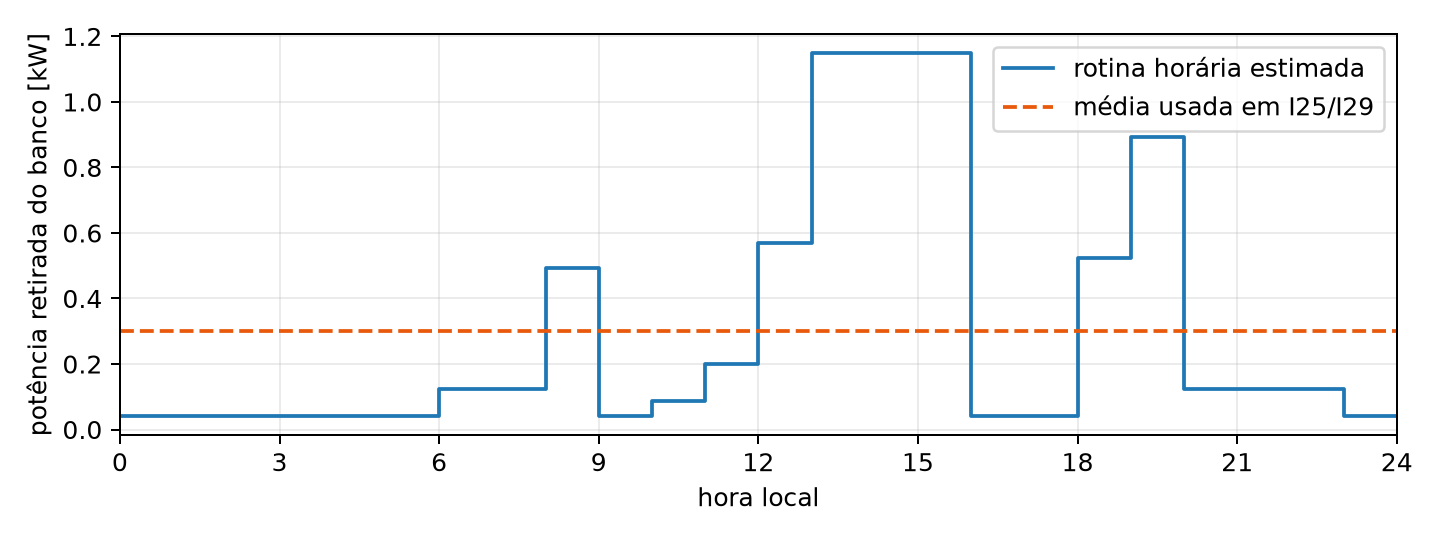
\includegraphics[width=0.9\linewidth]{i13_perfil_habitacao.png}
\caption{Perfil horário estimado da habitação e a aproximação por potência média.
As parcelas incluem perdas de conversão e consumo em vazio; os ciclos semanais são rateados por dia.}
\label{fig:perfil_servicos}
\end{figure}


\begin{table}[htbp]\centering\small
\caption{Dimensões de integração, em metros; uma unidade por aparelho.}
\begin{tabularx}{\linewidth}{lXp{5cm}}
\toprule Elemento & Material / tipo & Envelope [m] \\\midrule
Midea MRC10B2 & gabinete metálico/isolante, frigobar compressor & $0{,}450\times0{,}472\times0{,}860$ \\
LG VC2 & gabinete metálico, tambor de lavagem e secagem & $0{,}620\times0{,}600\times0{,}850$ \\
Electrolux IE3TP & superfície vitrocerâmica, indução & $0{,}358\times0{,}280\times0{,}062$ \\
Porta Potti 365 & conjunto sanitário polimérico & $0{,}427\times0{,}383\times0{,}414$ \\
Cama / colchão & compensado/aço/espuma; materiais do item 17 & $1{,}950\times1{,}350\times0{,}120$ (colchão) \\
Tanques limpa/cinza & polímero, envelopes estimados & $0{,}80\times0{,}50\times0{,}25$ / $0{,}70\times0{,}50\times0{,}20$ \\
Boiler Quick B3 & reservatório metálico de 15 L, 500 W & $0{,}40^3$, envelope estimado \\
Assentos, 2 & bancos com cinto e mecanismos OEM & massa/dimensões individuais na tara; não desmembradas \\
\bottomrule\end{tabularx}\end{table}

\designsec{Suspensão e direção}
\itemmark{14}
São mantidas a suspensão McPherson dianteira com barra estabilizadora, o eixo traseiro
com molas parabólicas e a direção por pinhão/cremalheira com assistência elétrica.

Nos 81 casos do layout A, as cargas variam de \SIrange{\FrenteMinA}{\FrenteMaxA}{kg}
na dianteira e \SIrange{\TrasMinA}{\TrasMaxA}{kg} na traseira. Os limites por eixo OEM não foram obtidos; dimensões e massas individuais da suspensão
e da direção permanecem incluídas na tara, sem desmembramento publicado. A estimativa $a_y=gt/(2h_{CG})\approx\SI{0,95}{g}$ considera corpo
rígido e serve apenas para comparar layouts; não é limite real de estabilidade.

\designsec{Chassi e carroceria}
\itemmark{15}
Mantém-se o monobloco de aço L3H2: \qtyproduct{5,998 x 2,050 x 2,592}{m},
entre-eixos de \SI{4,035}{m} e compartimento de \qtyproduct{3,705 x 1,870 x 1,932}{m}
\cite{fiatsk}. A conversão utiliza 18 chapas calculadas, com massa bruta de \SI{33,1}{kg}.

A maior utilização, 0,99, ocorre na chapa do boiler cheio (22 kg): 160×100×6 mm,
5g lateral+1g vertical, CG a 0,30 m e excentricidade de 0,25 m.
Essas chapas não foram somadas ao item 18 porque substituem reservas sem massa líquida
conhecida. Somadas integralmente, levam a \SI{\MassaComChapas}{kg}, ainda com margem
de \SI{\MargemComChapas}{kg}. Carga do teto e ancoragens OEM seguem sem confirmação.

\itemmark{16}
A carroceria, o para-brisa, os vidros e as portas dianteiras/lateral/traseiras são OEM
e já integram os \SI{2790}{kg} de base. A conversão acrescenta uma janela de acrílico duplo, moldura de poliuretano e tela, Dometic S4
9104104526, de \qtyproduct{544 x 330}{mm}, recorte 499×298 mm e massa de 4 kg \cite{janelaS4}.
Requadro e nervuras exigem conferência no veículo.

Os \SI{288}{mm} livres à frente do deck não atendem aos \SI{390}{mm} mínimos da Micro
Heki; portanto não se instala claraboia \cite{microheki,microespaco}. Preveem-se entrada
vedada dos cabos de teto e duas passagens protegidas de água no piso.

A parede tem ArmaFlex de 32 mm e revestimento de 6 mm. Com os filmes de ar,
$R''=\SI{1,340}{m^2.K/W}$ e $U=\SI{0,746}{W/(m^2.K)}$ \cite{armaflex}.
O modelo usa 39,16 m² opacos, 4,60 m² de vidro ($U_v=5{,}7$, fator solar 0,60) e
pontes térmicas de 10 W/K, resultando em $UA=\SI{65,44}{W/K}$.
A reserva de janelas/proteções é 16 kg: 4 da janela e 12 dos demais elementos.

\designsec{Geometria, montagem e massa}
As posições dos componentes, a massa e a aerodinâmica ligam as escolhas de projeto
aos resultados de consumo e temperatura. A Figura~\ref{fig:dependencias} apresenta
as grandezas transferidas entre essas análises.
\begin{figure}[htbp]
\centering
\begin{tikzpicture}[fluxo]
\node[frente] (p1) at (0,3.2) {P1 · estrutura, freios,\\massa e custo};
\node[frente] (p3) at (5.6,3.2) {P3 · carroceria,\\CAD e CFD};
\node[frente] (p4) at (11.2,3.2) {P4 · motor\\e dinâmica};
\node[frente] (p2) at (0,0) {P2 · baterias,\\elétrica e cabos};
\node[frente] (p5) at (5.6,0) {P5 · solar, autonomia\\e viagem};
\node[frente] (p7) at (11.2,0) {P7 · arrefecimento\\e bateria};
\node[frente] (p6) at (2.8,-2.6) {P6 · interior\\e conforto};
\draw[seta] (p1.north) to[out=20,in=160] node[rot,above] {massa e CG} (p4.north);
\draw[seta] (p3) -- node[rot] {$C_d$, $A$} (p4);
\draw[seta] (p3) -- node[rot] {área do teto} (p5);
\draw[seta] (p4) -- node[rot,align=center] {$e(v)$,\\potências} (p5);
\draw[seta] (p1) -- node[rot] {massa} (p5);
\draw[seta,<->] (p2) -- node[rot,above=2pt,align=center] {geração, bancos,\\interface CC} (p5);
\draw[seta] (p4) -- node[rot,align=center] {perdas,\\corrente} (p7);
\draw[seta] (p6) -- node[rot,align=center] {perfil de\\consumo} (p2);
\draw[seta] (p6) -- node[rot,align=center] {consumo da\\habitação} (p5);
\draw[seta,dashed] (p2) -- node[rot,align=center] {massas e preços\\(todas as frentes)} (p1);
\end{tikzpicture}
\caption{Mapa de dependências entre as frentes. As setas indicam a grandeza transferida; a interface CC
entre os bancos de serviço e de tração é hipótese de estudo.}
\label{fig:dependencias}
\end{figure}

\itemmark{17}
O modelo mede 5,981 m de comprimento, 2,079 m de largura (2,491 com espelhos) e 2,688 m
com o deck. Difere do catálogo em 17 mm a menos no comprimento e 29 mm a mais na largura.
O layout A foi escolhido pelo acesso aos equipamentos; o B deixa apenas 6 mm para a lava e seca.
\begin{figure}[htbp]
\centering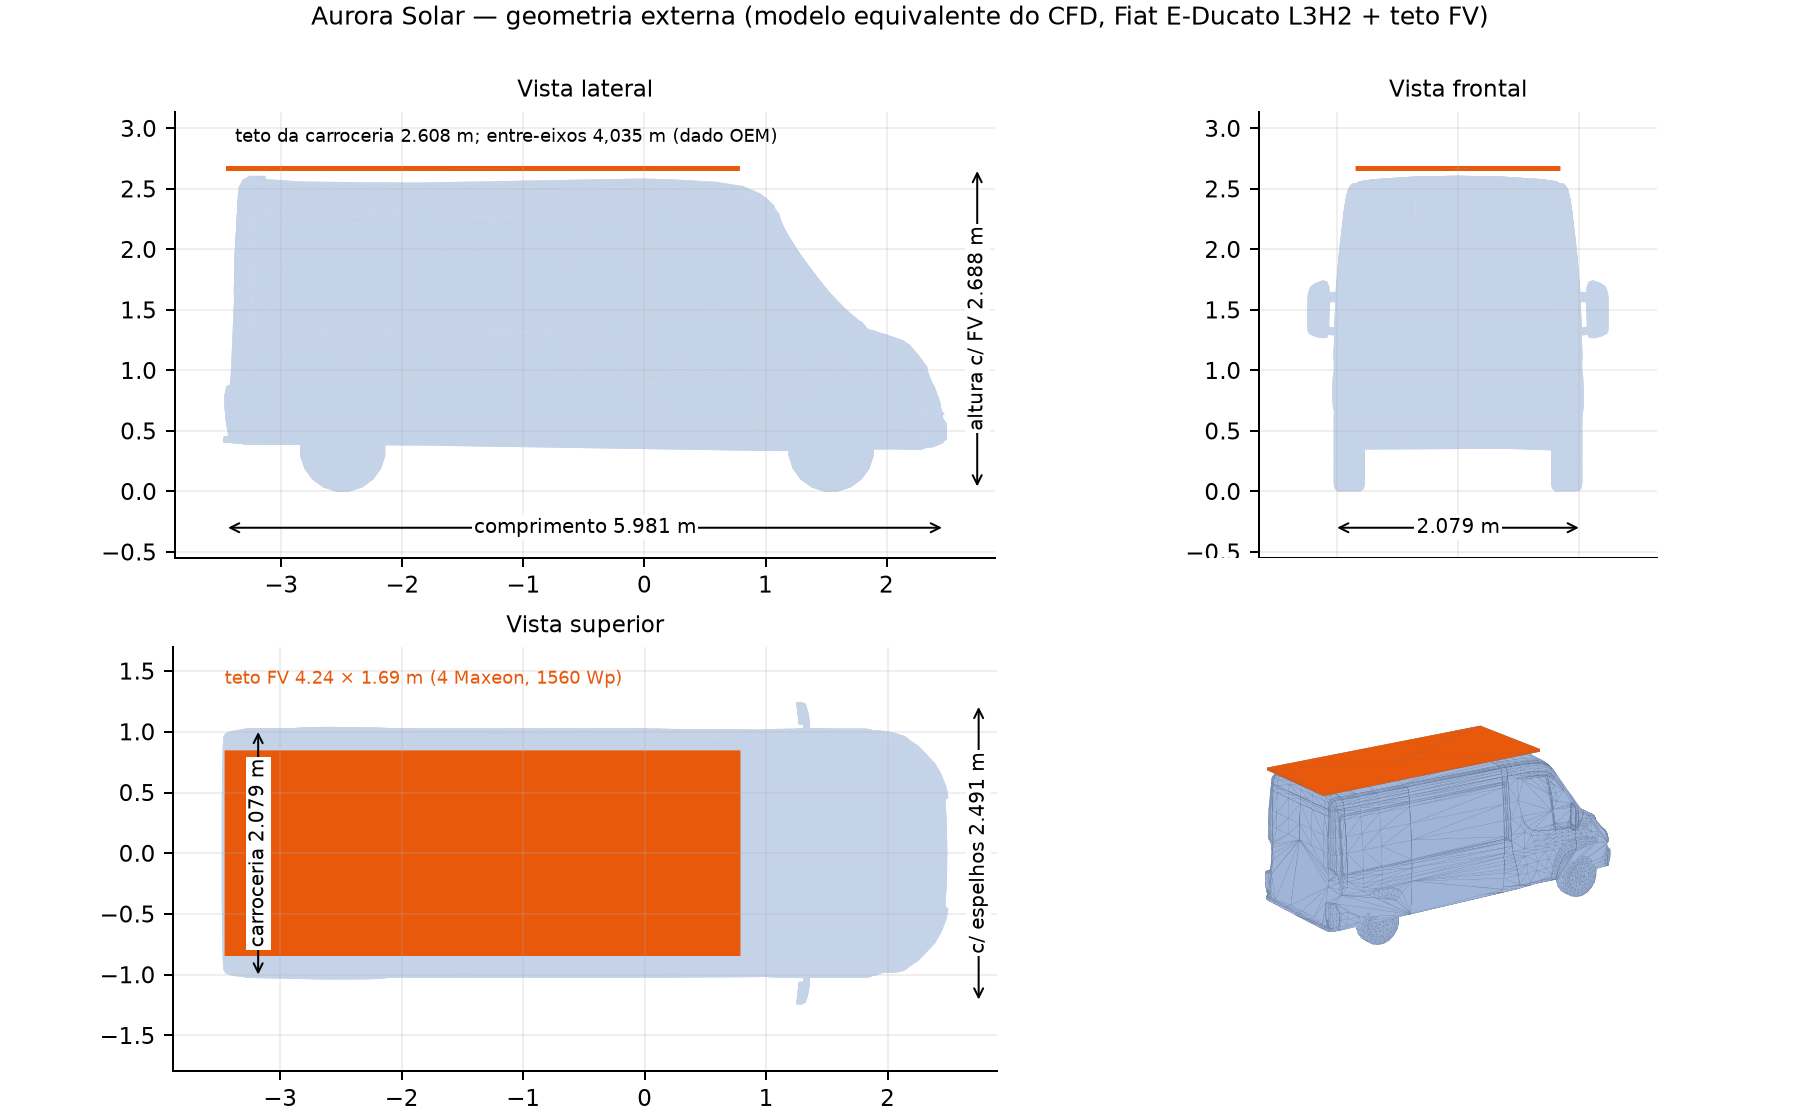
\includegraphics[width=\linewidth]{i17_vistas_exterior.png}
\caption{Vistas lateral, superior e frontal e perspectiva da geometria externa usada
no CFD. A carroceria deriva da malha Fiat Ducato 2014 do OpenX Assets
(razor24, 2019; Dogan Ulus, 2025; MPL-2.0 e CC-BY-4.0) \cite{openx}, ajustada às cotas
L3H2.}
\label{fig:vistas}
\end{figure}
\begin{figure}[htbp]
\centering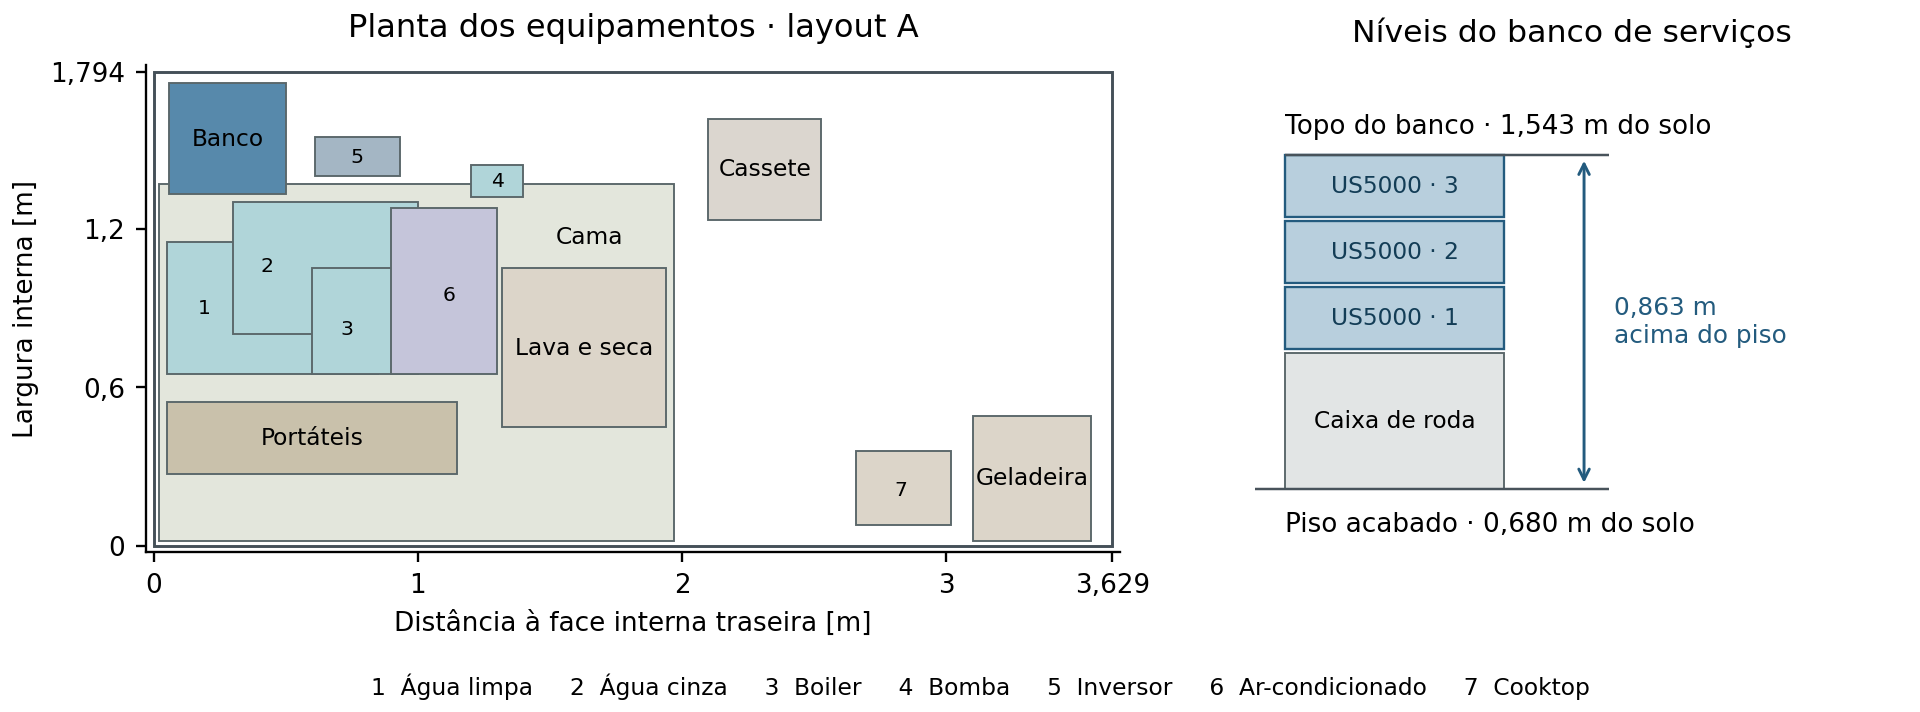
\includegraphics[width=\linewidth]{i17_layout_interno.png}
\caption{Layout A com os envelopes da montagem final. O banco US5000 vai de 0,360 a \SI{0,863}{m} acima do piso acabado, cuja altura é de \SI{0,680}{m} em relação ao solo.}
\label{fig:layout}
\end{figure}
\begin{figure}[htbp]
\centering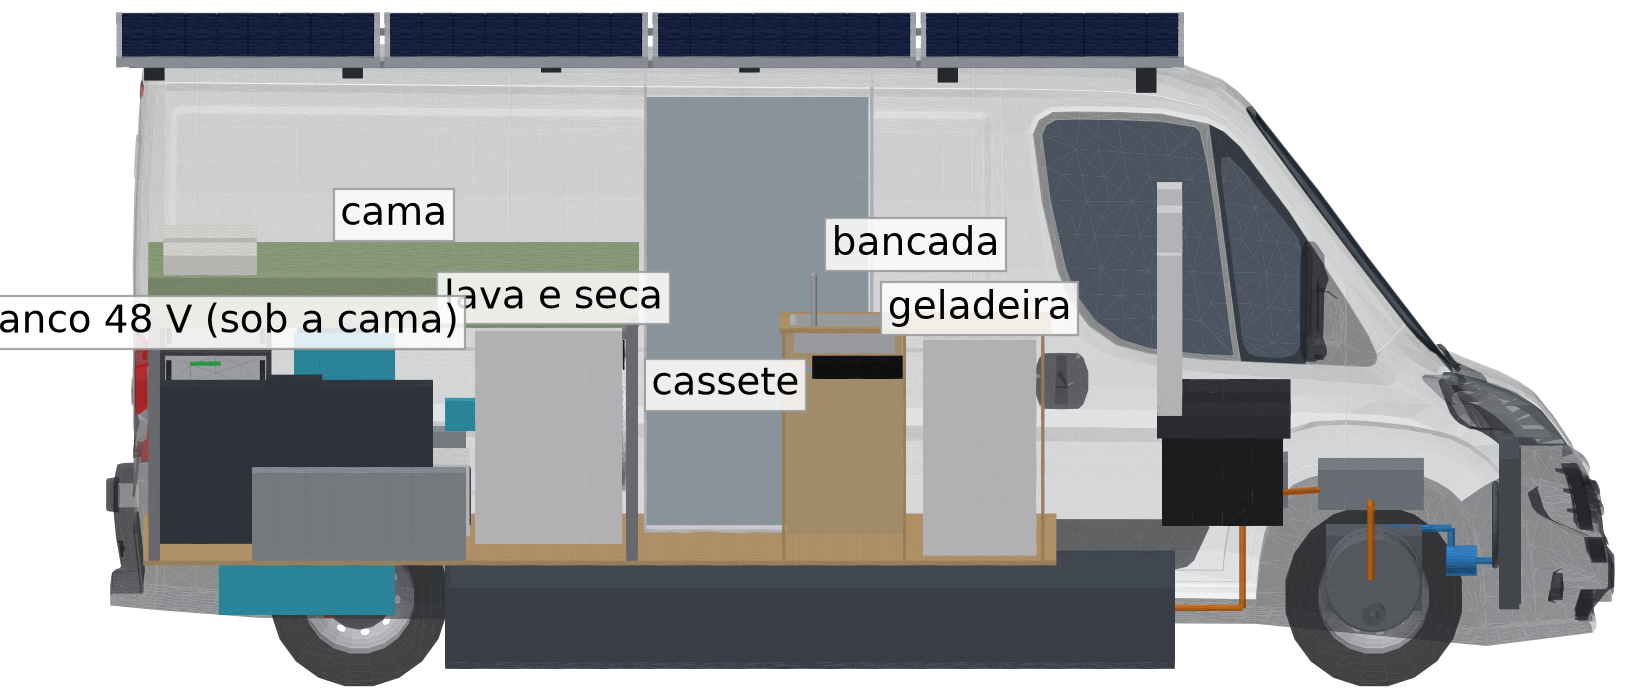
\includegraphics[width=\linewidth]{cad_corte.png}
\caption{Corte longitudinal com o lado direito da carroceria removido: bateria de tração e
motor OEM sob o piso, layout A e deck solar sobre trilhos apoiados no teto abaulado.}
\label{fig:corte}
\end{figure}

O banco US5000 fica sob a cama, com topo a 0,863 m do piso, 117 mm abaixo do estrado
e 67 mm abaixo do quadro. Há folgas de apenas 1 mm ao poste e 2 mm ao acesso do inversor,
a conferir fisicamente. O suporte apoia no piso e sobre a caixa de roda estimada;
sua utilização é 0,41 no aço e 0,31 nos parafusos a 5g.
A elevação isolada de 0,320 m do banco acrescenta 9,4 mm ao CG do inventário.

A cama utiliza compensado de 30 mm, quadro S235 50×50×3 mm e quatro postes 45×45×4 mm.
Foram verificados duas pessoas de 80 kg, ajoelhamento com fator 2, 3g vertical sem
ocupantes e 5g lateral. Adotam-se $E_{comp}=8$ GPa e resistência de cálculo 15,33 MPa,
hipóteses a confirmar no painel; para o aço, $E=210$ GPa e $f_y=235$ MPa.
\[
 I=\frac{b^4-(b-2t)^4}{12},\quad \sigma=\frac{M}{I/(b/2)},\quad
 \delta=\frac{5qL^4}{384EI}\leq L/300.
\]
\begin{table}[H]\centering\small
\caption{Item 17 — verificação da cama por elementos idealizados; utilização 1 é o limite.}\label{tab:cama}
\begin{tabularx}{\linewidth}{Xrrr}
\toprule
Caso & Utilização & Flecha [mm] & Limite [mm] \\
\midrule
A estrado & 0,027 & 0,11 & 2,17 \\
B estrado concentrada & 0,422 & 1,28 & 2,17 \\
A longarina central & 0,187 & 2,40 & 6,33 \\
A longarina lateral & 0,093 & 1,20 & 6,33 \\
A travessa & 0,128 & 0,61 & 4,33 \\
A poste & 0,009 & -- & -- \\
C longarina 3g & 0,159 & -- & -- \\
C estrado 3g & 0,020 & -- & -- \\
D poste 5g lateral & 0,833 & -- & -- \\
D2 parafusos parede 5g & 0,117 & -- & -- \\
B longarina concentrada & 0,624 & 6,02 & 6,33 \\
D3 parafusos bases 5g & 0,485 & -- & -- \\
\bottomrule
\end{tabularx}
\end{table}

O máximo é \UtilCama, nos postes; a longarina central também atende ao ajoelhamento.
Quatro M8 classe 8.8 por base, com braço de 60 mm, atendem no aço; a amarração por
quatro M8 à parede é complementar. Soldas, bases e arrancamento na carroceria não
foram validados. A montagem por envelopes não constitui desenho de fabricação.

\itemmark{18}
A massa calculada é \textbf{\SI{\MassaNom}{kg}}, incluindo duas pessoas de 80 kg,
60 kg de bagagem e 100 L de água. A margem ao PBT é \SI{\MargemNom}{kg}.
O CG é $(\CgX;\CgY;\CgZ)$ m; as cargas são \SI{\EixoDianteiro}{kg} na dianteira
e \SI{\EixoTraseiro}{kg} na traseira.
\begin{table}[H]\centering\small
\caption{Massa montada com a cama redimensionada; somas do inventário.}\label{tab:massa}
\begin{tabularx}{\linewidth}{Xr}
\toprule
Parcela & Massa [kg] \\
\midrule
Equipamentos domésticos, sanitário e climatização & 130,4 \\
Banco de serviços e inversor & 150,1 \\
Tanques, cabos, hidráulica, suportes e proteções solares & 81,0 \\
Teto FV, portáteis com bolsas e fixações solares & 175,0 \\
Cama: estrado, quadro, postes e colchão do inventário & 116,3 \\
Mobiliário, piso, isolamento e revestimentos & 255,0 \\
Ocupantes, bagagem e alimentos & 245,0 \\
Água limpa/cinza/cassete e boiler (100 L no total) & 100,0 \\
Veículo-base (inclui bateria de tração) & 2790,0 \\
\textbf{Total} & \textbf{4042,8} \\
\bottomrule
\end{tabularx}
\end{table}

A massa líquida da estrutura da cama é de \SI{\MassaExtraCama}{kg}, descontada a
reserva de 12 kg para evitar dupla contagem. O envelope estrutural de 30 kg de colchão/roupa é conservador; o inventário tem
12 kg de colchão. A margem varia de \SIrange{\MargemMinA}{\MargemMaxA}{kg} nos casos do
layout A. As chapas gerais são tratadas separadamente no item 15; cumprir o PBT não
comprova os limites por eixo.

\designsec{Aerodinâmica e resistências ao movimento}
\itemmark{19}
A silhueta equipada mede \SI{4,8954}{m^2}. O CFD fornece $C_d=\CdValor$ sobre a área
original de \SI{4,82784}{m^2}, equivalente a $C_d=0{,}61295$ sobre a silhueta total;
em ambos, $C_dA=\SI{3,00068}{m^2}$.

Utilizou-se OpenFOAM/SIMPLE, RANS $k$--$\omega$ SST, domínio de 55×20×10 m, entrada de
22,22 m/s, solo móvel, rodas paradas e funções de parede. As três malhas convergiram
iterativamente, mas a variação entre elas é oscilatória: não comprova incerteza de 1\%
nem permite GCI/Richardson \cite{stern,celik}.
\GCItabela
A área inclui espelhos e deck; mudar a referência altera $C_d$, mas preserva $C_dA$.
A energia usa $C_d=0{,}625$ e $A=4{,}82784$ m², dentro da faixa observada. O caso sem deck
mantém domínio, fundo 55×20×10, refinamento superficial 5--6, contornos, rodas e área
de referência; o total cai para 524.241 células ao retirar o refinamento do deck.
\begin{table}[H]\centering\small
\caption{Itens19/20/26 — comparação aerodinâmica com a mesma massa; potências no lado da bateria.}\label{tab:deck}
\begin{tabularx}{\linewidth}{Xrrrrrr}
\toprule
Caso & $C_d$ & $C_dA$ [m²] & $P_{40}$ [kW] & $P_{80}$ [kW] & $e_{40}$ [kWh/km] & $e_{80}$ [kWh/km] \\
\midrule
Com deck & 0,6215 & 3,001 & 9,10 & 32,68 & 0,228 & 0,408 \\
Sem deck & 0,5555 & 2,682 & 8,83 & 30,53 & 0,221 & 0,382 \\
\bottomrule
\end{tabularx}
\end{table}

O deck acrescenta \SI{0,319}{m^2} a $C_dA$. Para compensar a perda dos \SI{5,94}{kWh/dia}
do teto, seria necessário rodar mais de \SI{\DeckKmEmpateQuarenta}{km/dia} a 40 km/h ou
\SI{\DeckKmEmpateOitenta}{km/dia} a 80 km/h. Por isso ele é mantido.
A comparação isola o arrasto, mantendo a massa; os 84 kg de portáteis recolhidos
entram no rolamento. Rodas sem rotação, $y^+$ médio de 304,6 na carroceria e geometria
equivalente limitam a interpretação; não houve validação experimental.
\begin{figure}[htbp]
\centering\includegraphics[width=\linewidth]{cfd_cp.png}
\caption{Coeficiente de pressão na carroceria e no deck solar (malha fina, \SI{80}{km/h}): estagnação no para-brisa e na grade, sucção na borda do teto e no início do deck.}
\label{fig:cp}
\end{figure}
\begin{figure}[htbp]
\centering\includegraphics[width=\linewidth]{cfd_plano.png}
\caption{Velocidade no plano de simetria: campo publicado da malha fina à iteração 344. Observam-se a aceleração na região do teto e o déficit de velocidade na esteira.}
\label{fig:cfdplano}
\end{figure}

\itemmark{20}
Além do arrasto aerodinâmico, o movimento encontra resistência nos pneus.
Adota-se $C_r=0{,}012$, com sensibilidade 0,008--0,016. Essa resistência vem
principalmente da histerese: o pneu deforma e dissipa parte da energia como calor.
O rótulo C2 classe C indica 0,0068--0,0080 em tambor; o valor maior é hipótese
conservadora para asfalto, temperatura e carga \cite{euLabel,gillespie}.
Com a massa do projeto, $F_r=C_rmg=\SI{\RolamentoNom}{N}$; não há ensaio do pneu adotado.

\itemmark{21}
Em pista plana, sem vento, essas duas parcelas são expressas por
\begin{equation}
F_a = \tfrac{1}{2}\rho C_d A v^2, \qquad F_r = C_r m g .
\end{equation}
A soma das resistências é mostrada na Figura~\ref{fig:forcas}. A \SI{40}{km/h}, $F_a = \SI{205}{N}$ e $F_r = \SI{\RolamentoNom}{N}$
(total \SI{681}{N}); a \SI{80}{km/h}, $F_a = \SI{819}{N}$ e total \SI{1295}{N}. O arrasto
supera o rolamento a partir de cerca de \SI{60}{km/h}.
\begin{figure}[htbp]
\centering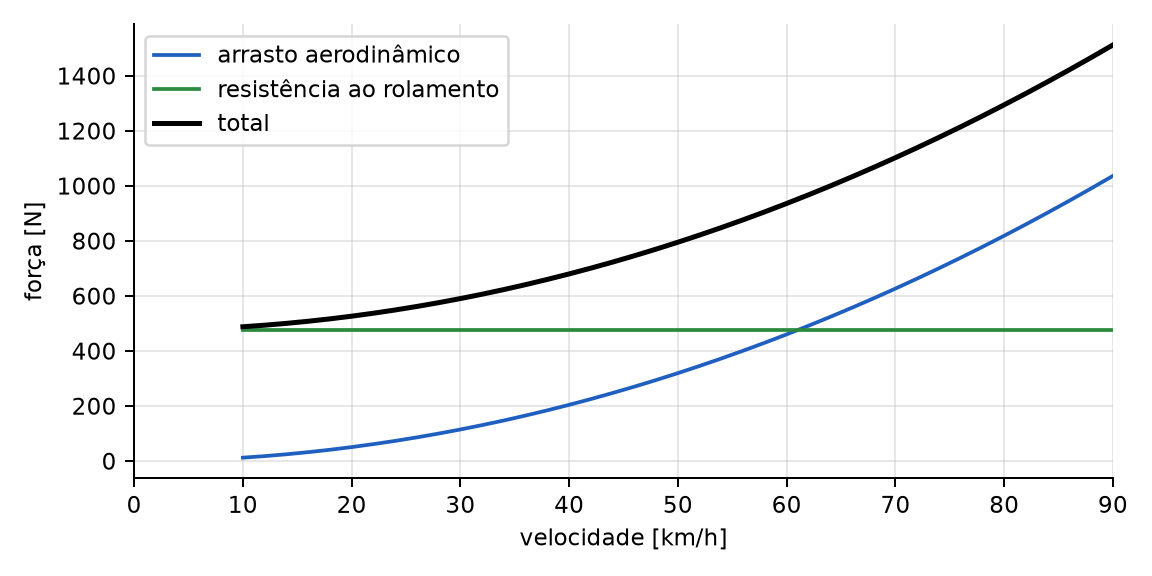
\includegraphics[width=0.75\linewidth]{i21_forcas_resistivas.png}
\caption{Forças resistivas no plano, sem vento ($C_d = 0{,}625$, $C_r = 0{,}012$,
$m = \SI{\MassaNom}{kg}$).}
\label{fig:forcas}
\end{figure}
A sensibilidade de 8100 casos (massa, velocidade, rampa de $\pm6\,\%$, vento de
$\pm\SI{10}{m/s}$, $C_r$, $C_d$ e densidade) tem demanda máxima de \SI{140}{kW} nas rodas
(\SI{90}{km/h}, rampa de 6\,\%, vento contrário de \SI{10}{m/s}, \SI{4250}{kg}), abaixo do
pico do motor.

\itemmark{22}
Multiplicando a força pela velocidade, obtém-se a potência necessária para manter
o movimento. A Figura~\ref{fig:potencias} mostra a demanda nas rodas de \SI{7,56}{kW} a
\SI{40}{km/h} e \SI{28,78}{kW} a \SI{80}{km/h}; na bateria, com rendimento 0,90 e
\SI{700}{W} de auxiliares, \SI{\PotenciaBateriaQuarenta}{kW} e \SI{\PotenciaBateriaOitenta}{kW}.
\begin{figure}[htbp]
\centering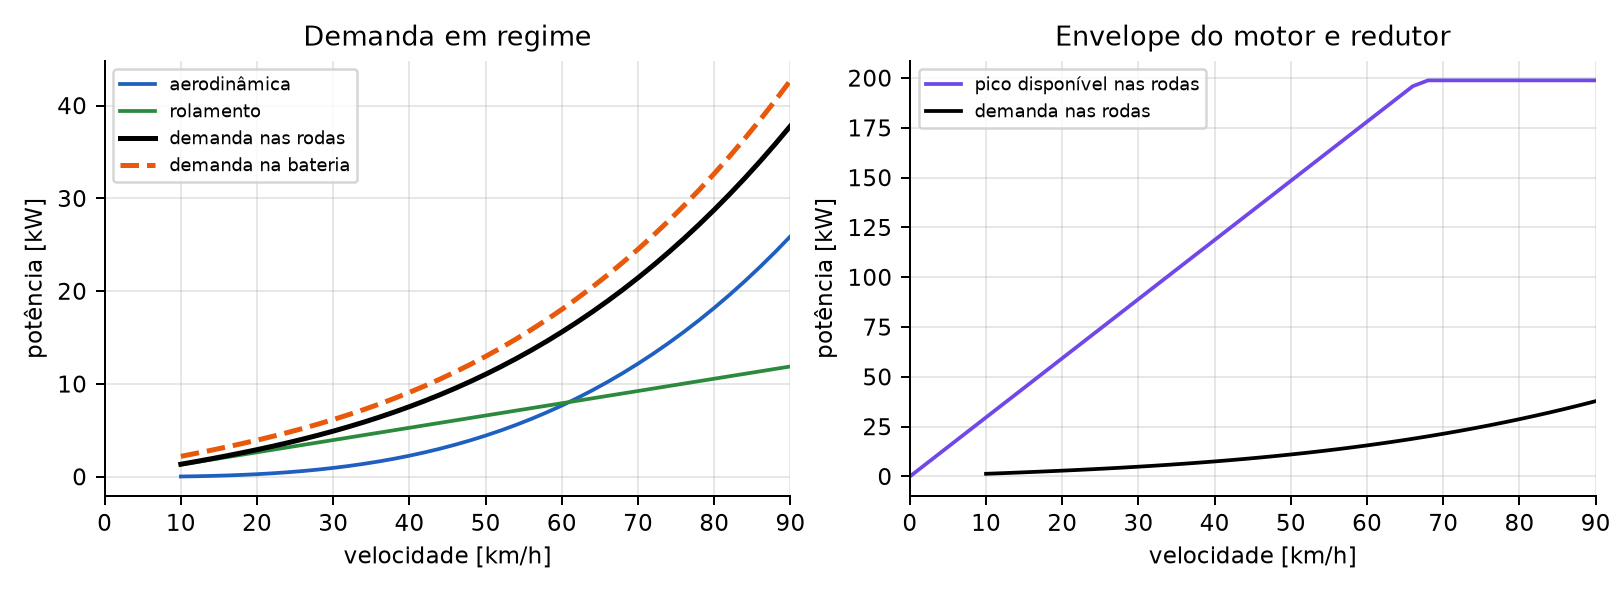
\includegraphics[width=\linewidth]{i22_potencias.png}
\caption{Demanda em regime e envelope de pico disponível nas rodas,
$P_{disp}=\eta_{red}\min(T_{max}iv/r,P_{max})$. Relação 10 e rendimento do redutor 0,97 são
hipóteses; o pico não é potência contínua garantida, nem substitui o limite de aderência.}
\label{fig:potencias}
\end{figure}

\FloatBarrier
\subsection{Análise de Custo}
\itemmark{24}
O orçamento separa a aquisição do veículo, os equipamentos de conversão e uma
reserva de montagem, suportes e acabamento. As aquisições e os componentes fora dessa
reserva somam \textbf{R\$ \CustoComponentesMil\ mil}, com faixa de
R\$ \CustoComponentesMinMil--\CustoComponentesMaxMil\ mil. A rubrica mista acrescenta
R\$ \CustoRubricaMistaMil\ mil no nominal, levando o investimento total a
\textbf{R\$ \CustoProjetoMil\ mil}, ou aproximadamente R\$ 794 mil.

A reserva não discrimina materiais e mão de obra. Portanto, na hipótese nominal,
o custo de aquisição e materiais fica entre R\$ \CustoComponentesMil\ e
R\$ \CustoProjetoMil\ mil, conforme a parcela material dessa rubrica. O limite
superior inclui toda a reserva; não é uma soma apenas de componentes cotados.
Os câmbios de referência são USD/BRL 5,5146 e EUR/BRL 6,1748. Nas importações,
o cálculo soma CIF, II, IPI, PIS/COFINS e ICMS por dentro, totalizando R\$ 327 mil
em tributos. As alíquotas/faixas e fontes são registradas no orçamento \cite{ii35}.
\begin{table}[H]\centering\small
\caption{Orçamento por componente/rubrica; valores já incluem a hipótese tributária. Estimativas são identificadas na descrição.}\label{tab:custos}
\begin{tabularx}{\linewidth}{Xrrr}
\toprule
Componente ou rubrica & Qtd. & Nominal [mil R\$] & Faixa [mil R\$] \\
\midrule
Fiat E-Ducato L3H2 SK MY25 505.GG1.2 (sem IVA) & 1 & 618,86 & 580,38--664,53 \\
Maxeon 3 SPR-MAX3-390-COM, 4 unidades (preço do 400 W como referência) & 4 & 15,07 & 13,50--18,04 \\
Pylontech US5000 4,8 kWh & 3 & 29,67 & 26,57--35,50 \\
Victron MultiPlus-II GX 48/5000/70-50 & 1 & 10,63 & 9,52--12,72 \\
Victron SmartSolar MPPT 250/60-Tr (teto) & 1 & 4,52 & 4,05--5,41 \\
Victron SmartSolar MPPT 150/60-Tr (portáteis) & 1 & 3,82 & 3,42--4,57 \\
Dometic FreshWell 3000 (sob banco) & 1 & 24,44 & 21,89--29,25 \\
Reimo REMIfront IV, cortina de para-brisa Ducato 2021 (S8), art. 37482 (I32; preço com IVA, acesso 24/11/2026) & 1 & 4,99 & 4,47--5,97 \\
Thetford Porta Potti 365 & 1 & 1,36 & 1,21--1,62 \\
EcoFlow 400 W portátil & 4 & 22,85 & 22,85--22,85 \\
Frigobar Midea 93 L MRC10B2 220 V & 1 & 1,50 & 1,50--1,50 \\
Lava e seca LG VC2 (equivalente ao CV9011WC4A; menor preço do CV9013WC4) & 1 & 5,88 & 5,88--5,88 \\
Cooktop de indução Electrolux IE3TP 220 V & 1 & 0,44 & 0,44--0,44 \\
Isolamento termoacústico (estimativa) & 1 & 4,50 & 2,50--6,50 \\
Marcenaria, cama, bancada, assentos (estimativa) & 1 & 8,00 & 4,00--15,00 \\
Cabos, fusíveis, conversor 48/12 V, boiler, bomba, tanques, tubos (estimativa) & 1 & 12,00 & 8,00--18,00 \\
Montagem, suportes e acabamento (estimativa) & 1 & 25,00 & 15,00--40,00 \\
\textbf{Total} &  & 793,54 & 725,18--887,79 \\
\bottomrule
\end{tabularx}
\end{table}

A cama está nas rubricas de marcenaria/suportes; a cortina de EUR 458 está incluída
\cite{remifront}. O Renogy é alternativa e não é somado ao conjunto EcoFlow escolhido.
Preços de lista e faixas estimadas não constituem cotação.
\FloatBarrier
\clearpage
\subsection{Simulações}
As escolhas anteriores são avaliadas a seguir nas condições do enunciado. Primeiro,
analisam-se o aquecimento dos componentes e a capacidade de resfriamento; em seguida,
as resistências ao movimento permitem calcular desempenho, consumo e autonomia.
Em cada análise, as hipóteses, o modelo e os resultados são apresentados em conjunto.
Os estudos de malha, passo temporal e balanço de energia verificam a solução numérica;
não substituem validação experimental.
\begin{table}[htbp]
\centering\small
\caption{Condições utilizadas nos cálculos.}
\label{tab:cenario}
\setlength{\tabcolsep}{3pt}
\begin{tabular}{lll}
\toprule
Grandeza & Valor & Origem \\
\midrule
Local, data & São Carlos, 21/06, céu limpo & enunciado; INMET A711 \\
Ambiente & \SI{25}{\celsius}, UR 50\,\%, vento \SI{0}{m/s}, $\rho = \SI{1,10}{kg/m^3}$ & enunciado; altitude \\
Massa montada típica & \SI{\MassaNom}{kg} (2 pessoas, bagagem, \SI{100}{L} de água) & item 18 \\
Área de referência do $C_d$ & \SI{4,828}{m^2} & casco (item 19) \\
$C_d$ nos modelos de energia & 0,625 (sensibilidade 0,581--0,720) & item 19 \\
$C_r$ & 0,012 (faixa 0,008--0,016) & item 20 \\
Rendimento bateria--roda & 0,90 (faixa 0,85--0,95) & hipótese \\
Auxiliares de tração & \SI{700}{W} em movimento & hipótese \\
Bateria de tração & \SI{98}{kWh} úteis, \SI{400}{V}, LFP & Fiat SK \cite{fiatsk} \\
Banco de serviços & \SI{14,4}{kWh}, \SI{48}{V}, LFP & item 6 \\
Teto FV / portáteis & \SI{1560}{Wp} / \SI{1600}{Wp} (só parado) & item 8 \\
\bottomrule
\end{tabular}
\end{table}
\itemsec{33}{Temperatura dos freios durante a frenagem}
Durante a frenagem, os discos de freio convertem a energia cinética do carro em
energia térmica por meio do atrito. No ensaio prescrito, a velocidade cai de 30 para
10 m/s em cinco segundos, com temperatura inicial de 25 °C. Para a massa de
\SI{\MassaNom}{kg}, a energia cinética retirada é
\[
 \Delta E_c=\frac{m}{2}(v_0^2-v_f^2)\approx\SI{1,62}{MJ}.
\]
Descontando o trabalho do arrasto e do rolamento, o sistema de atrito dissipa cerca de
\SI{1,49}{MJ}. Os 108 km/h iniciais são uma condição de ensaio do componente prevista
no enunciado, acima do limitador de velocidade do veículo escolhido.

O calor é aplicado às pistas de atrito do disco. Adotam-se 70\% da frenagem no eixo
dianteiro e 90\% do calor de atrito absorvido pelos discos; o restante segue para as
pastilhas. A distribuição de temperatura no raio $r$ e na espessura $z$ é obtida pela
condução transiente, resolvida por Crank--Nicolson:
\[
 \rho c_p\frac{\partial T}{\partial t}
 =k\left[\frac{1}{r}\frac{\partial}{\partial r}
 \left(r\frac{\partial T}{\partial r}\right)
 +\frac{\partial^2T}{\partial z^2}\right].
\]
Usam-se as propriedades de ferro fundido apresentadas na Seção~\ref{item:3} e convecção
de 20/50 W/(m²K). A geometria e as propriedades são referências de cálculo,
sem confirmação do conjunto instalado por VIN \cite{topczewska}.

A Figura~\ref{fig:freios_termicos} reúne o campo ao fim dos cinco segundos e o histórico
do ponto mais quente. Sem regeneração, o pico superficial é
\textbf{\SI{\FreioPico}{\celsius}} na massa nominal e 312,49 °C no PBT. Com regeneração
hipotética de 40 e 80 kW, os máximos caem para \FreioRegenQuarenta\ e
\FreioRegenOitenta\ °C, respectivamente.
\begin{figure}[H]
\centering
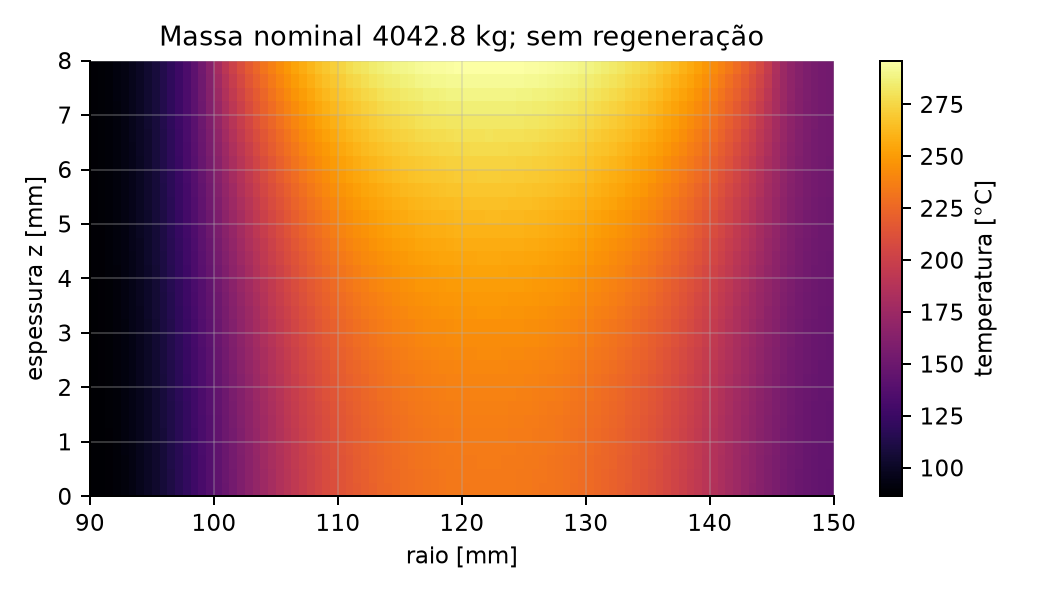
\includegraphics[width=0.49\linewidth]{i33_campo.png}\hfill
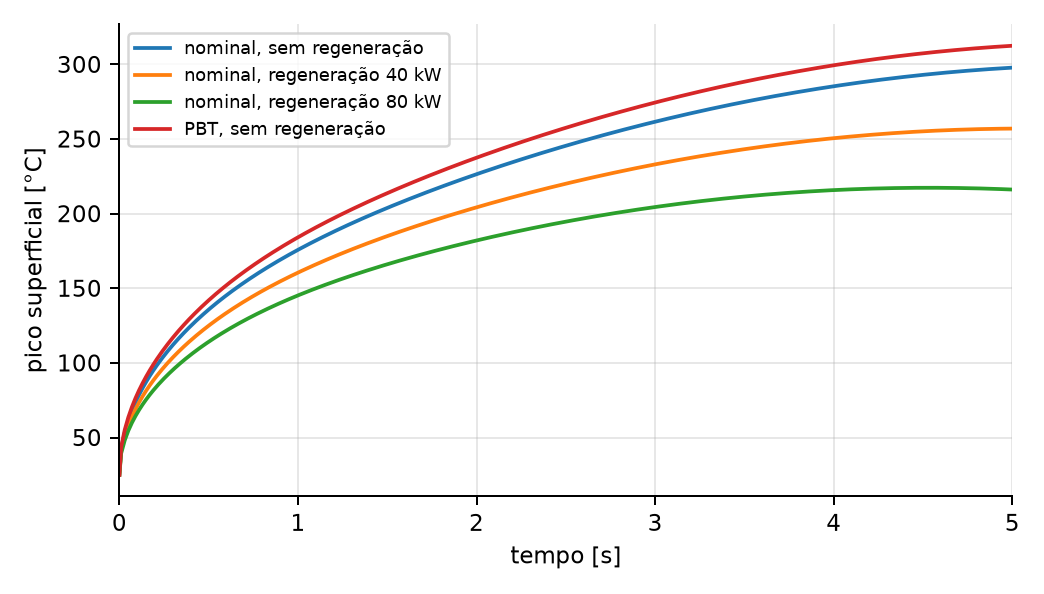
\includegraphics[width=0.49\linewidth]{i33_historico.png}
\caption{Temperatura no disco ao fim da frenagem, à esquerda, e evolução do pico
superficial para as massas e potências de regeneração comparadas, à direita.}
\label{fig:freios_termicos}
\end{figure}
O campo mostra que a pista de atrito aquece mais que as bordas e o interior do disco;
portanto, a temperatura média não representa o pico da superfície. A regeneração
reduz a parcela de energia que chega aos freios, mas sua aceitação pela bateria não
foi demonstrada. A comparação de quatro malhas, de 24×8 a 96×32, apresenta diferença
de cerca de 0,026 K no mesmo passo temporal; a verificação analítica 1D dá ordem 1,96.
Essas conferências sustentam a solução numérica, sem equivaler a um ensaio do freio.

\itemsec{30}{Temperatura nos fios de alimentação do motor}
Assim como nos freios, uma perda de energia provoca aquecimento: nos cabos, a fonte
é o efeito Joule. A potência mecânica de pico de 205 kW, acima da rotação de base, exige corrente de fase
RMS distinta da corrente CC da bateria:
\[
 V_{LL}=400/\sqrt2=\SI{283}{V},\qquad
 I=\frac{205000}{0{,}95\sqrt3\,283(0{,}90)}=\SI{489}{A}.
\]
Adotam-se rendimento do motor 0,95, fator de potência 0,90 e limite linear SVPWM.
No modo normal, 160 kW correspondem a 382 A; tensão de bateria menor eleva a corrente.

O campo $T(r,\theta)$ é resolvido por volumes finitos no cobre e no isolamento, com
$q^{\prime\prime\prime}=I^2R(T)/A$. A convecção de Churchill--Chu e a radiação são iteradas com a temperatura;
o contorno inclui conduíte, agrupamento e perda CA.
\begin{figure}[H]
\centering
\begin{tikzpicture}[fluxo]
\node[caixa] (p) at (0,0) {potência\\mecânica};
\node[caixa] (i) at (3.2,0) {corrente de fase\\$I = P/(\eta_m\sqrt3\, V_{LL}\, FP)$};
\node[caixa] (q) at (7.0,0) {geração Joule\\$q^{\prime\prime\prime} = I^2 R(T)/A$};
\node[caixa] (fv) at (11.0,0) {condução $r$--$\theta$\\(volumes finitos)};
\node[caixa] (bc) at (11.0,-2.0) {contorno: convecção\\(Churchill--Chu) e radiação};
\node[decisao] (cv) at (7.0,-2.1) {$T$ da superfície\\convergiu?};
\node[caixa] (t) at (2.9,-2.1) {$T_{\max}$ e\\critério de 125\,°C};
\draw[seta] (p) -- (i); \draw[seta] (i) -- (q); \draw[seta] (q) -- (fv); \draw[seta] (fv) -- (bc);
\draw[seta] (bc) -- (cv); \draw[seta] (cv) -- node[rot,above] {sim} (t);
\draw[seta] (cv) -- node[rot,right] {não: atualiza $R(T)$ e $h(T)$} (q);
\end{tikzpicture}
\caption{Balanço térmico do cabo: a resistência e o coeficiente de convecção dependem da
temperatura, por isso a solução é iterada até a temperatura de superfície convergir.}
\label{fig:fluxo_cabo}
\end{figure}
\begin{center}\small
\begin{tabular}{lcccc}
\toprule
Contorno (modo normal, \SI{382}{A}) & \SI{120}{mm^2} & \SI{150}{mm^2} & \SI{185}{mm^2} & \SI{240}{mm^2} \\
\midrule
Referência idealizada (\SI{25}{\celsius}, radiação plena) & 62 & 53 & 46 & 40 \\
Rota protegida (\SI{50}{\celsius}/\SI{70}{\celsius}) & 134 & 114 & 101 & 89 \\
Cofre do motor (\SI{60}{\celsius}/\SI{80}{\celsius}, conduíte) & \textbf{158} & 134 & \textbf{118} & 104 \\
\bottomrule
\end{tabular}
\end{center}
A tabela permite comparar o mesmo carregamento elétrico em três instalações: as
temperaturas estão em °C. Com critério de 125 °C, a menor seção é \textbf{185 mm² no cofre}
e 150 mm² em rota protegida. O pico de 205 kW por 180 s acrescenta cerca de 1--3 K;
no cabo de 185 mm² do cofre, pode durar aproximadamente sete minutos antes de 125 °C.
As seções 185/240 mm² são derivadas por geometria calibrada e exigem ficha específica.
Não se altera o chicote OEM: o cálculo é requisito para conferi-lo. Contornos, bitolas
derivadas de catálogo e terminais precisam de validação da instalação.
\begin{figure}[H]
\centering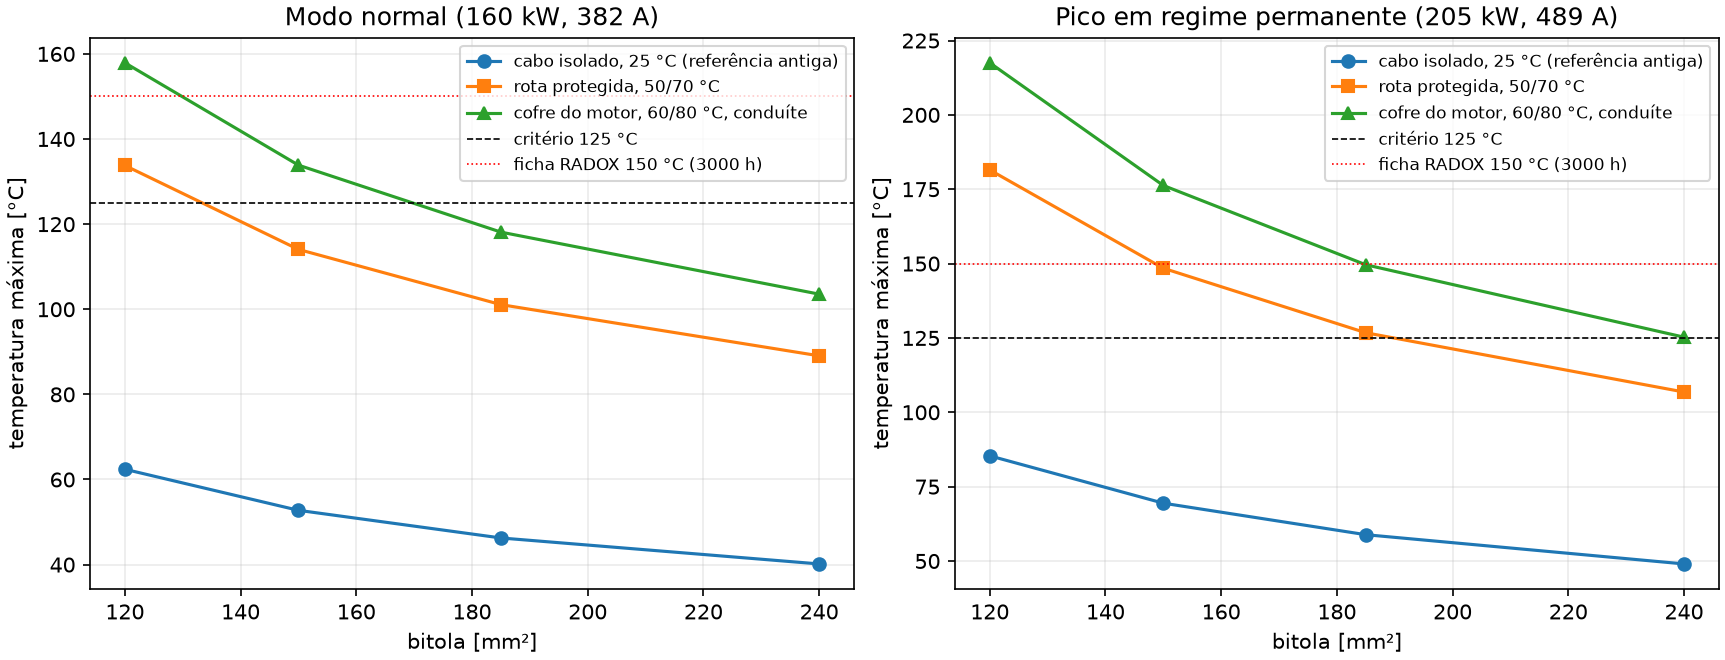
\includegraphics[width=\linewidth]{i30_cabos.png}
\caption{Temperatura máxima em função da bitola, no modo normal e no pico
permanente, para os três contornos térmicos.}
\end{figure}


A Figura~\ref{fig:cabo_campo} mostra como o aquecimento se distribui no condutor e
no isolamento caso a potência de pico fosse mantida até o equilíbrio. Esse caso
permanente é distinto do pico de duração limitada discutido acima.
\begin{figure}[H]\centering
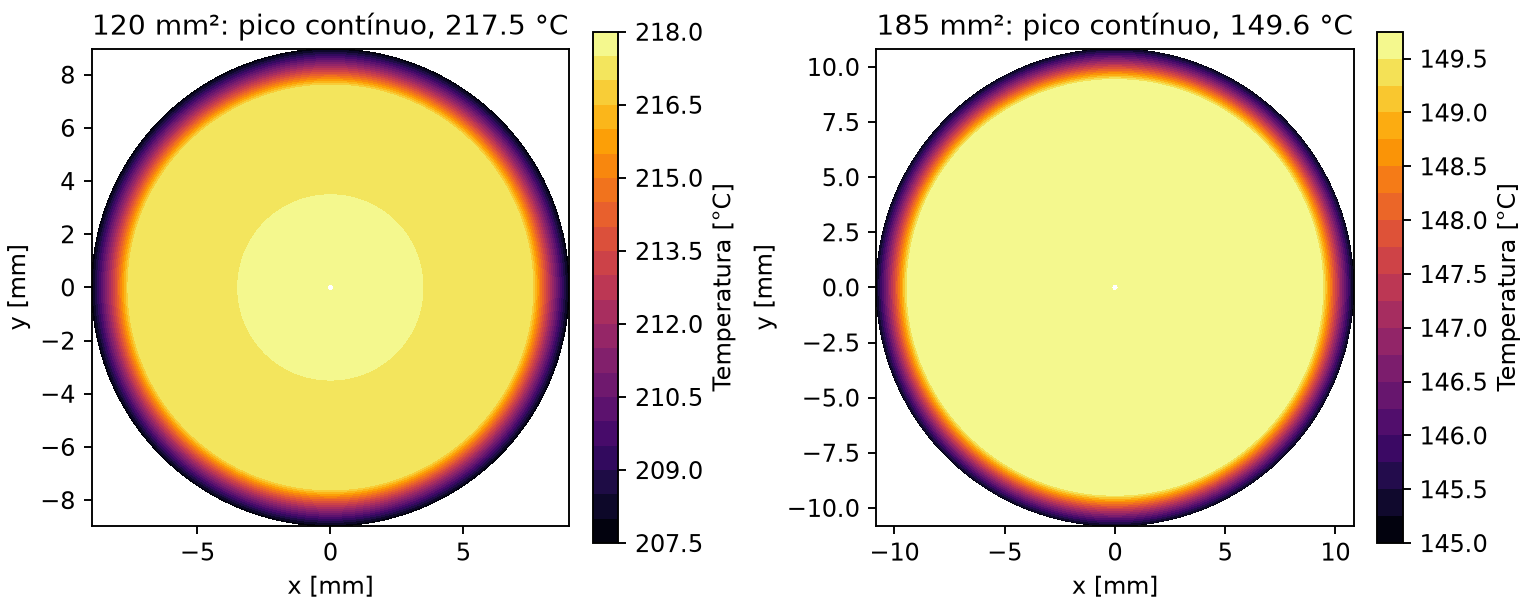
\includegraphics[width=\linewidth]{i30_campo.png}
\caption{Campo $T(x,y)$ na seção dos cabos a 489 A, no cofre, se o pico fosse
mantido até o regime. O contorno angular uniforme torna o campo radialmente simétrico;
a discretização resolve os dois materiais em $r$--$\theta$. A duração real do pico é tratada à parte.}
\label{fig:cabo_campo}
\end{figure}

\itemsec{31}{Aquecimento da cabine fechada}
Na cabine, o aquecimento decorre principalmente da radiação solar absorvida pela
carroceria e transmitida pelos vidros. Para avaliar a condição sem climatização,
a cabine começa às 6h a 25 °C, sem passageiros, ventilação ou ar-condicionado.
O balanço de zona única considera geração solar por face e perdas pela envoltória:
\[
 C\frac{dT}{dt}=\dot Q_{solar}-UA(T-T_a),\quad C=\SI{200}{kJ/K},\quad UA=\SI{65,4}{W/K}.
\]
Ao meio-dia, resulta em \textbf{49,1 °C}, com pico diário de 49,6 °C às 14h07.
O CFD 3D transiente fornece média de \textbf{50,3 °C}, máxima de 53,1 °C e
estratificação de cerca de 3 K. Nas malhas de 2400/8100/19200 células, a média varia
0,23 K; reduzir o passo de 0,1 para 0,05 s altera 0,001 K.
A Figura~\ref{fig:termica_cabine} mostra a distribuição espacial correspondente à convecção natural.
\begin{figure}[H]
\centering\includegraphics[width=0.85\linewidth]{i31_cabine.png}
\caption{Campos de temperatura e velocidade na cabine fechada (convecção natural).}
\label{fig:termica_cabine}
\end{figure}
A diferença entre média e máxima decorre da estratificação do ar. A temperatura de
equilíbrio da zona única não descreve esse gradiente; por isso os dois modelos são
apresentados juntos. A elevação acima de 25 °C motiva a avaliação do ar-condicionado
na seção seguinte.


\itemsec{32}{Capacidade do ar-condicionado}
Para retirar os ganhos de calor e manter 25 °C com exterior a 33 °C e UR de 50\%, somam-se transmissão, sol,
pessoas, aparelhos e ventilação:
\[
 \dot Q=UA\Delta T+\dot Q_{opacos}+\dot Q_{vidros}
 +n(q_s+q_l)+\dot Q_{eq}+\dot m_{as}\Delta h.
\]
São $\Delta T=8$ K, $UA=65{,}4$ W/K, $q_s/q_l=75/55$ W por pessoa e
$\dot Q_{eq}=100$ W. A ventilação inclui calor sensível e latente por psicrometria.
Nas paredes, $\dot Q_{opacos}=\sum UA\alpha I/h_o$; nos vidros,
$\dot Q_{vidros}=\sum gA_vI$, com $\alpha=0{,}3$, $h_o=8$ W/(m²K) e $g=0{,}6$.
$I$ é irradiância [W/m²], $A$ área [m²] e $\dot m_{as}$ vazão de ar seco [kg/s].
\begin{table}[htbp]
\centering\small
\caption{Carga, margem frente aos \SI{2,7}{kW} do FreshWell 3000 e potência elétrica (COP 2,5).}
\label{tab:i32margem}
\begin{tabular}{lrrr}
\toprule
Caso & Carga [kW] & Margem [kW] & Elétrica [kW] \\
\midrule
1 pessoa, \SI{30}{m^3/h} & 2,52 & $+0,18$ & 1,01 \\
2 pessoas, \SI{30}{m^3/h} & 2,65 & $+0,05$ & 1,06 \\
2 pessoas, \SI{62}{m^3/h} (CO$_2$) & 2,87 & $-0,17$ & 1,15 \\
2 pessoas, \SI{62}{m^3/h}, cortina fechada & 2,31 & $+0,39$ & 0,92 \\
\bottomrule
\end{tabular}
\end{table}

O COP é a razão entre frio removido e potência elétrica: $COP=\dot Q/P_{el}$.
Adota-se 2,5 (sensibilidade 2--3), pois a curva real do FreshWell nessa condição não foi publicada.
\begin{figure}[H]
\centering
\begin{tikzpicture}[fluxo]
\node[caixa] (s) at (0,1.8) {sol nas faces\\e nos vidros (pvlib)};
\node[caixa] (u) at (0,0.6) {condução $UA\,\Delta T$};
\node[caixa] (o) at (0,-0.6) {ocupantes e\\equipamentos};
\node[caixa] (v) at (0,-1.8) {ventilação sensível\\e latente (psicrometria)};
\node[caixa] (bal) at (4.2,0) {balanço de energia\\da cabine};
\node[caixa] (t31) at (8.0,1.0) {item 31: $T(t)$ interna\\(cabine fechada)};
\node[caixa] (q32) at (8.0,-1.0) {item 32: carga de\\resfriamento $\dot Q$ a 25\,°C};
\node[caixa] (pe) at (11.6,-1.0) {potência elétrica\\$P = \dot Q/\mathrm{COP}$};
\foreach \n in {s,u,o,v} \draw[seta] (\n.east) -- (bal.west);
\draw[seta] (bal) -- (t31); \draw[seta] (bal) -- (q32); \draw[seta] (q32) -- (pe);
\end{tikzpicture}
\caption{Mesmos ganhos térmicos. Na cabine fechada (item 31) eles aquecem o ar; com o
ar-condicionado (item 32) a temperatura é fixada e o balanço dá a carga de resfriamento e, pelo COP, a
potência elétrica.}
\label{fig:fluxo_cabine}
\end{figure}

O para-brisa recebe 1,11 kW solares. A cortina refletiva REMIfront IV fechada com o
veículo parado reduz esse ganho por um fator IAC=0,5, hipótese de atenuação interna
\cite{remifront,ashrae}. A carga cai para \textbf{2,31 kW}, margem de 0,39 kW frente
aos 2,7 kW nominais. Com IAC de 0,3--0,7, a margem fica em 0,17--0,61 kW.

Em $\dot m_{as}\Delta h$, $\Delta h$ é a diferença de entalpia do ar úmido [J/kg de ar seco].
Na missão o veículo está parado ao meio-dia. Sem cortina, reaparece o déficit de
0,17 kW com duas pessoas e 62 m³/h. IAC e capacidade real a 33/25 °C não foram ensaiados.
\begin{figure}[H]
\centering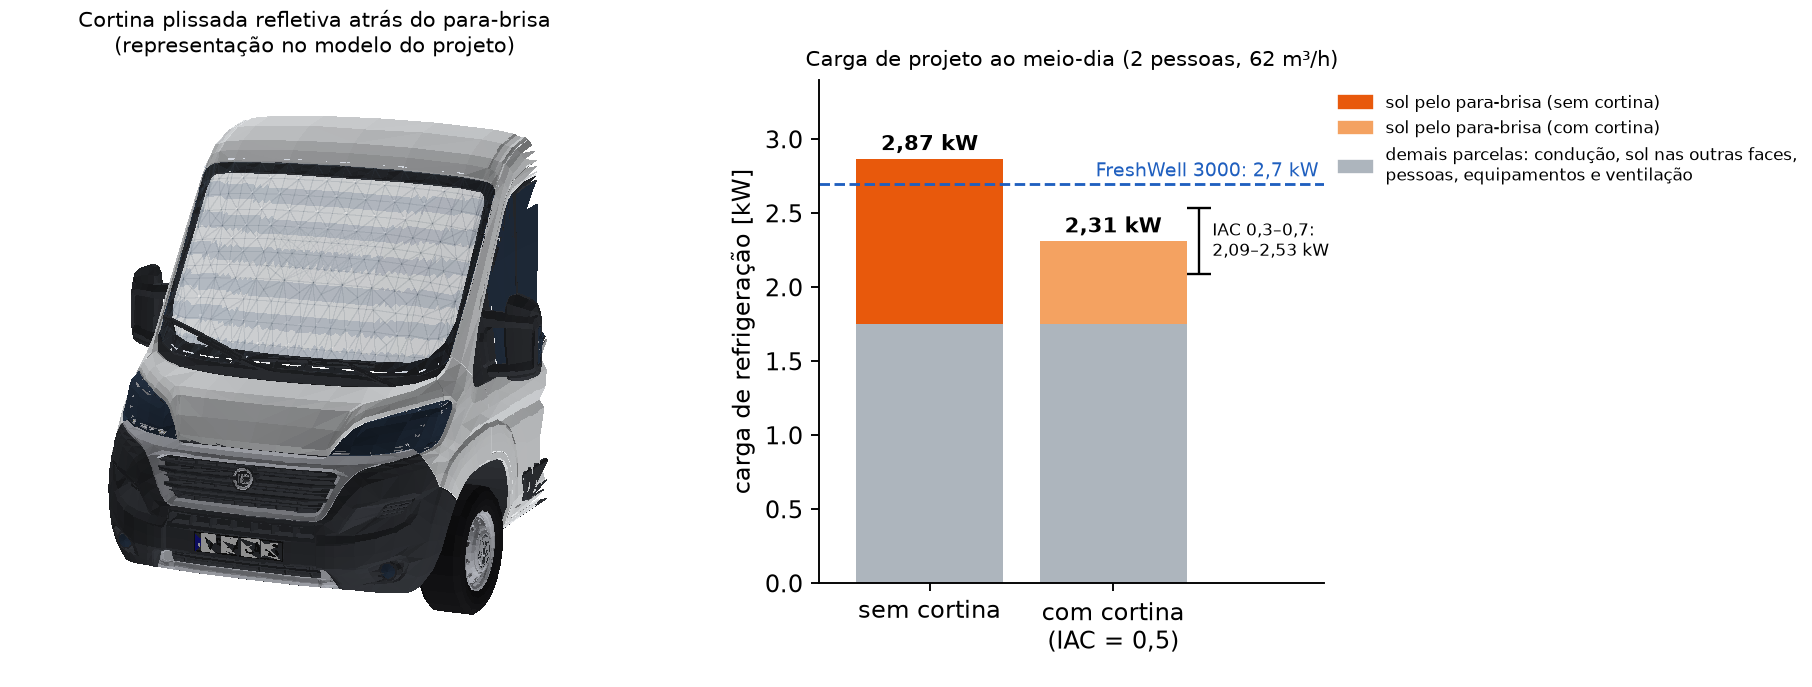
\includegraphics[width=\linewidth]{i32_cortina.png}
\caption{À esquerda, a cortina plissada refletiva fechada atrás do para-brisa, desenhada
sobre o modelo exterior do projeto (representação esquemática, não a geometria do produto); à
direita, a carga de projeto ao meio-dia sem e com a cortina, com a faixa de IAC de 0,3 a 0,7 e a
capacidade nominal do FreshWell 3000.}
\label{fig:cortina}
\end{figure}

\itemsec{34}{Temperatura da bateria durante a recarga}
O aquecimento elétrico também ocorre na bateria durante a recarga. Comparam-se
potências de 20 e 80 kW na mesma faixa de SOC, de 20 a 80\%, com bateria e fluido inicialmente a 25 °C.
O circuito $P=U_{oc}I+RI^2$ fornece a corrente; o calor é $I^2R+IT\,\partial U_{oc}/\partial T$.
O modelo de dois nós integra bateria e fluido:
\begin{align*}
 C_b\dot T_b&=\dot Q-UA_{bc}(T_b-T_c),\\
 C_c\dot T_c&=UA_{bc}(T_b-T_c)-UA_{ca}(T_c-T_a).
\end{align*}
Com 20 kW, a carga leva \textbf{2,96 h} e termina em \textbf{25,9 °C}; com 80 kW,
\textbf{0,76 h} e \textbf{32,0 °C}. O nominal usa massa de 650 kg, $c_p=900$ J/(kgK),
20 kg de fluido, resistência nominal de \SI{0,06}{\ohm} e coeficiente entrópico nulo.
As faixas são $R=0{,}03$--$0{,}12\,\Omega$, entropia de $-0{,}02$ a +0,02 V/K,
$UA_{bc}=125$--500 W/K e $UA_{ca}=250$--1000 W/K.

Nos 486 casos, a temperatura final varia em 22,8--30,9 °C a 20 kW e 25,1--45,0 °C
a 80 kW. Três casos atingem 45 °C antes do alvo e interrompem a carga em SOC 71--76\%.
A varredura inclui massa, resistência, condutâncias e entropia; o balanço fecha abaixo de
$2\times10^{-7}$ J.
A Figura~\ref{fig:termica_bateria} mostra que a recarga de maior potência termina antes, mas provoca maior aquecimento.
\begin{figure}[H]
\centering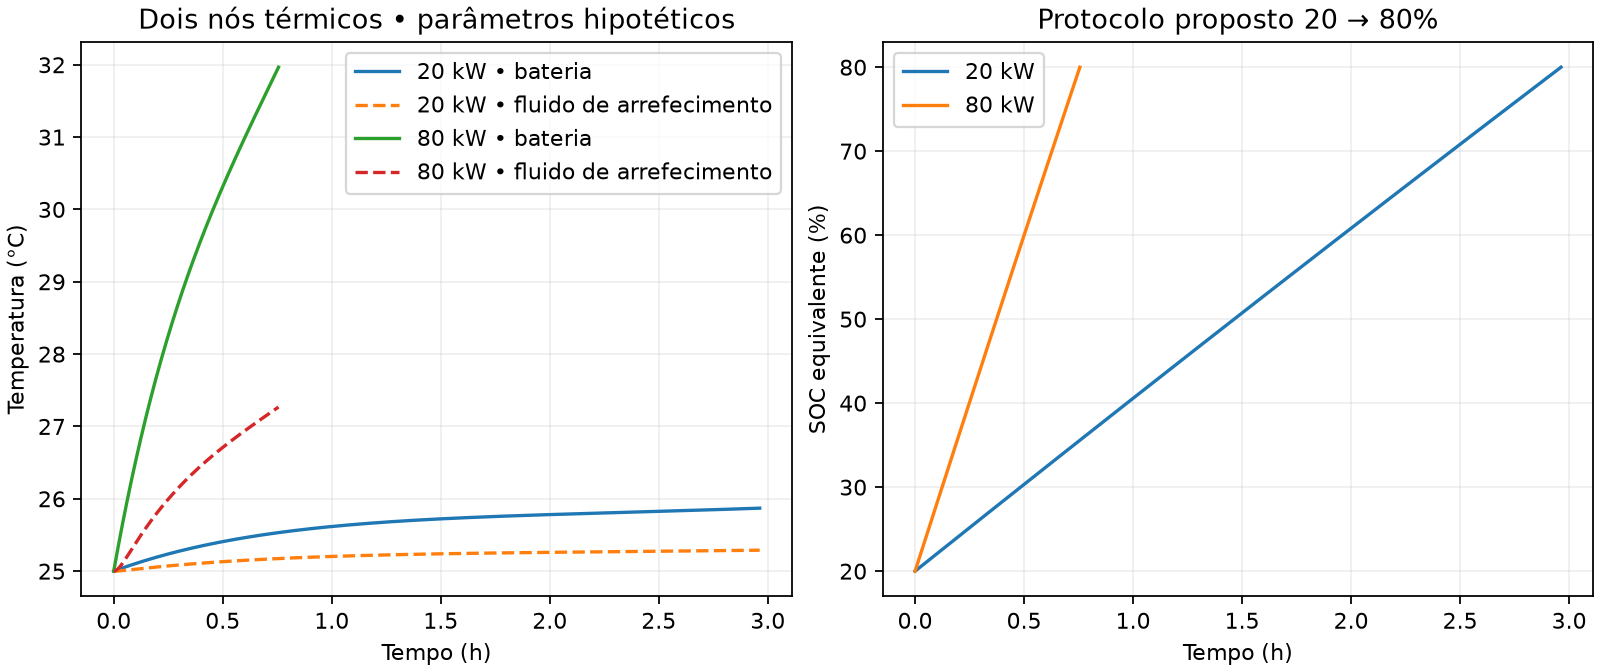
\includegraphics[width=0.85\linewidth]{i34_bateria.png}
\caption{SOC e temperaturas da bateria e do fluido de arrefecimento nas cargas de 20 e 80 kW.}
\label{fig:termica_bateria}
\end{figure}

A média nominal, isoladamente, esconde a sensibilidade ao calor gerado no pack.
A Figura~\ref{fig:bateria_parametros} isola resistência e entropia em um subconjunto
dos 486 casos, mantendo 500 kg e $UA_{bc}/UA_{ca}=125/250$ W/K.
A resistência maior eleva $I^2R$, enquanto o termo entrópico pode aquecer ou resfriar
na convenção de corrente adotada. O asterisco marca interrupção antes do SOC de 80\%.
\begin{figure}[H]\centering
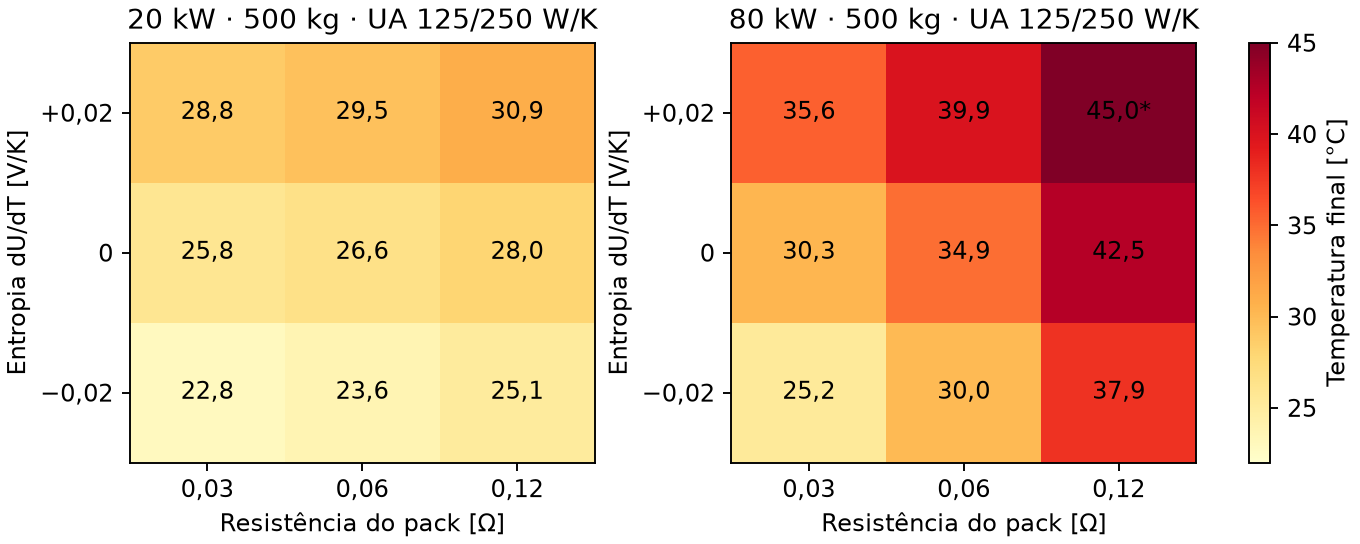
\includegraphics[width=0.9\linewidth]{comparacao_bateria.png}
\caption{Temperatura final ao variar resistência e entropia em cargas de 20 e 80 kW;
asterisco indica parada ao atingir o limite hipotético de 45 °C.}
\label{fig:bateria_parametros}
\end{figure}



No pior caso ($R=0{,}12\,\Omega$, $\partial U/\partial T=0{,}02$ V/K, 500 kg,
$UA_{bc}/UA_{ca}=125/250$ W/K), a carga de 80 kW para em 45 °C após 0,66 h;
partindo a 35 °C, após 0,37 h. A geração interna chega a 6,35 kW.
Um resfriador de 3--5 kW térmicos não garante a rejeição desse calor no extremo:
para rejeitar 6,35 kW com bateria a 45 °C e fluido a 25 °C, seriam necessários
$UA_{bc}\ge318$ W/K e ao menos 6,35 kW térmicos de capacidade instantânea.
Esse é um requisito condicional para o circuito da bateria; massa e custo adicionais
dependem da seleção de um equipamento e da capacidade do sistema original.

\itemsec{35}{Vazão de arrefecimento e desempenho do radiador}
Para controlar o aquecimento do trem de força, o circuito deve transportar as perdas
do motor e do inversor até o radiador. Na potência de pico, com rendimento combinado
de 90\%, a carga térmica é
$\dot Q=205(1/0{,}90-1)+0{,}096=\SI{22,9}{kW}$.
O encontro da curva Bosch PCE2-XL com a perda de pressão do circuito, calculada por
Darcy--Weisbach/Haaland, fornece \textbf{31,9 L/min} (0,557 kg/s) a 71,6 kPa:
96 W elétricos, 38 W hidráulicos e eficiência de 40\% \cite{bosch}.

O radiador de fluxo cruzado usa $UA=1000$ W/K e 1 kg/s de ar. Pela relação
$\dot Q=\dot m c_p(T_{in}-T_{out})$, o fluido entra a \textbf{66,8 °C} e retorna a
\textbf{55,1 °C}. A solução de 64×64 células confere com $\varepsilon$--NTU, erro de
$5\times10^{-6}$. Com rendimento de 85\%, a carga sobe a 36,3 kW e a entrada a 91,4 °C;
a potência máxima do motor é de curta duração.
A Figura~\ref{fig:arrefecimento_termico} relaciona a vazão obtida pela bomba às temperaturas calculadas no trocador.
\begin{figure}[H]
\centering
\includegraphics[width=0.49\linewidth]{i35_ponto_operacao.png}\hfill
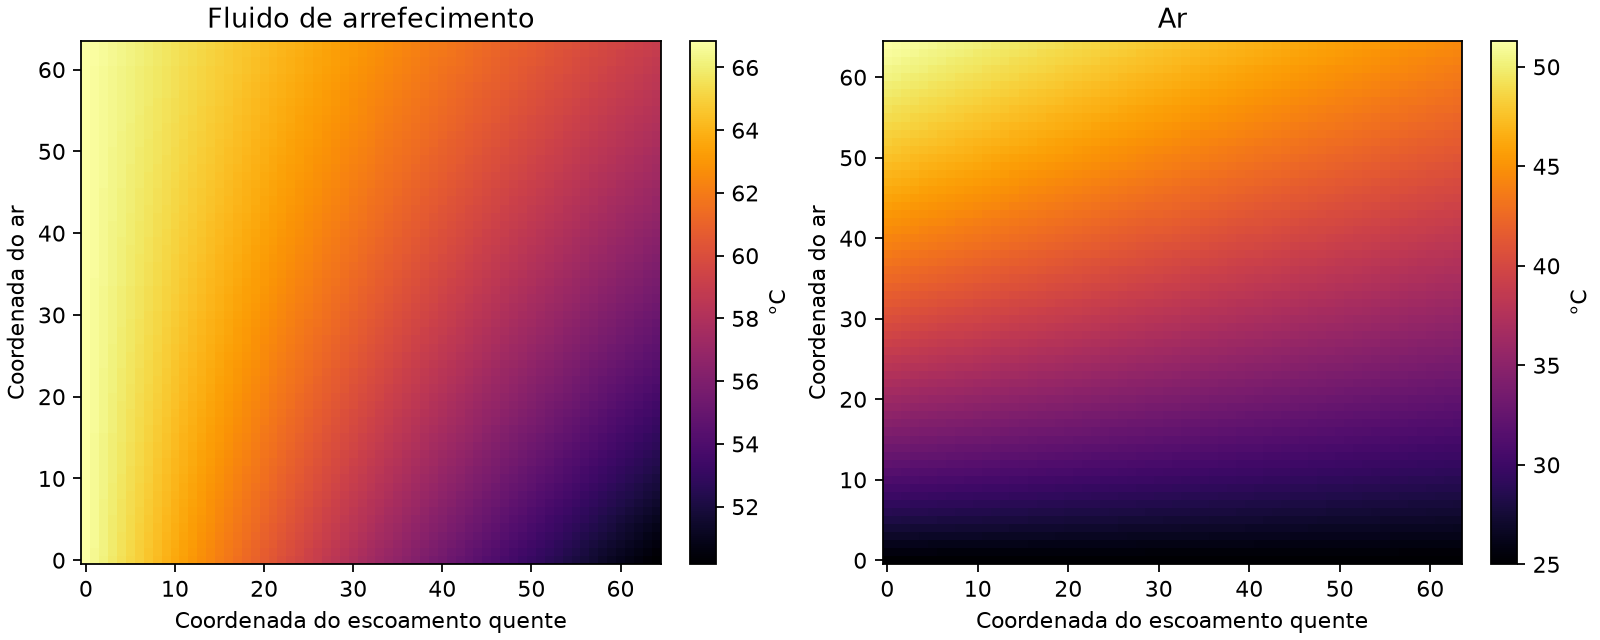
\includegraphics[width=0.49\linewidth]{i35_radiador.png}
\caption{Ponto de operação da bomba e perfis de temperatura do fluido de arrefecimento e do ar.}
\label{fig:arrefecimento_termico}
\end{figure}


A escolha do radiador depende da temperatura admissível de entrada no inversor.
Adota-se, como meta a confirmar, 65 °C. Com $UA=1000$ W/K, os 66,8 °C calculados
não atendem; para 22,9 kW, exige-se $UA\ge1093$ W/K. A Figura~\ref{fig:arrefecimento_parametros}
mostra o efeito de variar $UA$ e rendimento combinado, mantendo a vazão de ar de
1 kg/s. Uma redução de rendimento aumenta o calor que o mesmo radiador precisa rejeitar.
\begin{figure}[H]\centering
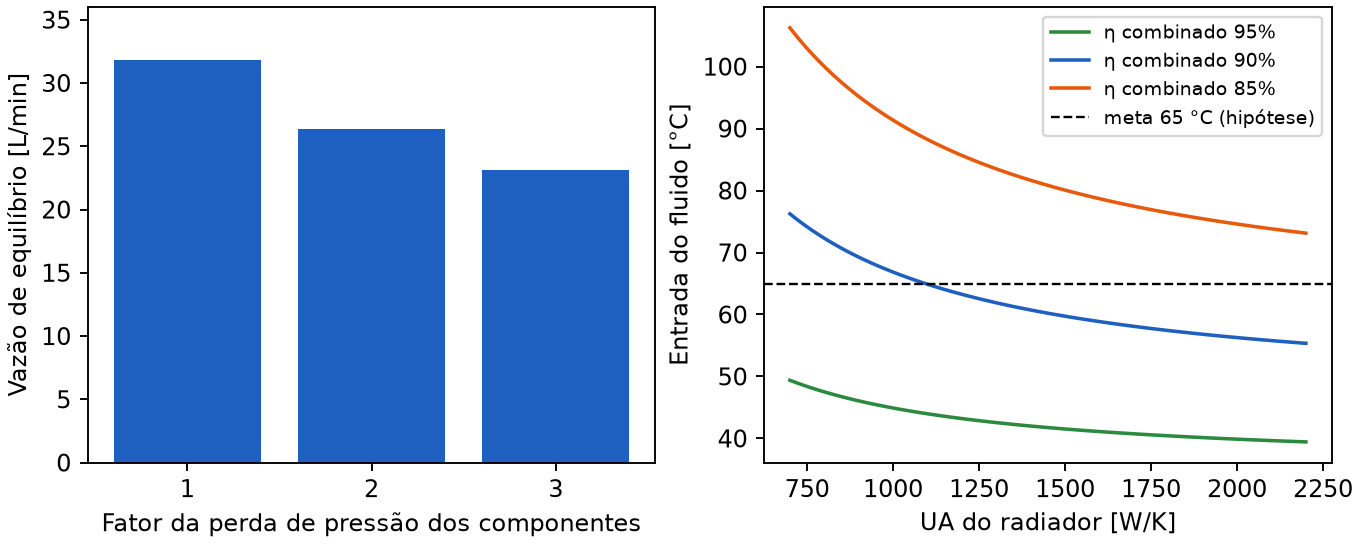
\includegraphics[width=0.95\linewidth]{comparacao_arrefecimento.png}
\caption{Sensibilidade da vazão às perdas dos componentes, à esquerda, e da temperatura
de entrada ao $UA$ e ao rendimento combinado, à direita.}
\label{fig:arrefecimento_parametros}
\end{figure}
Os componentes respondem por 48,5 dos 71,6 kPa de perda de pressão, ou 68\%.
Ao duplicar e triplicar essa parcela, a vazão de equilíbrio cai de 31,9 para
26,4 e 23,1 L/min, respectivamente. A seleção da bomba depende, portanto,
da resistência hidráulica real dos componentes, além do comprimento de mangueira.

Se o redutor compartilhar o mesmo circuito, seus 6,15 kW a $\eta_{red}=0{,}97$
elevam a carga total a 29,02 kW. Nesse caso, a entrada seria 78,1 °C com
$UA=1000$ W/K, e a meta de 65 °C exigiria $UA\ge1952$ W/K. Já o pior caso
resistivo sustentado, de 140 kW nas rodas, corresponde a aproximadamente 144 kW
no motor e perdas motor/inversor de 11--13 kW. O pico contínuo de 205 kW é,
assim, um envelope conservador; a ligação hidráulica do redutor ainda precisa ser confirmada.

A estimativa de cavitação usa pressão atmosférica de 91,5 kPa, pressão de vapor
hipotética de 55 kPa a 90 °C e perda na sucção de 10 kPa. A altura líquida positiva de sucção disponível (NPSH) é
2,6 m sem pressurização e 12,3 m com tampa de 100 kPa(g). A pressão de vapor e as
perdas de sucção são hipóteses; sem o NPSH requerido da bomba, a margem contra
cavitação não está comprovada.

Na proteção térmica,
adota-se parada da bateria de tração a 45 °C, também hipotética; o limite de óleo
do redutor é desconhecido. O US5000 admite carga de 0 a 50 °C e descarga de
$-10$ a 50 °C \cite{pylontech}; o MultiPlus-II fornece 4000 W a 25 °C e reduz a
potência com a temperatura. Essas condições precisam ser verificadas na instalação.

A geometria estimada do núcleo não substitui a curva $UA$/vazão do fabricante.
Os circuitos OEM e suas massas permanecem na tara; qualquer chiller ou ventilação
adicional só entra no inventário após seleção e substituição líquida das reservas.

\itemsec{28}{Velocidade máxima e aceleração}
A ficha limita a variante de 4250 kg a \textbf{90 km/h}. Com $i=10$,
$\eta_{red}=0{,}97$ e $\mu=0{,}8$, a integração fornece
\textbf{\SI{\AcelNoventa}{s} de 0--90} e, retirando o limitador apenas no modelo,
\textbf{\SI{\AcelCem}{s} de 0--100}. Nos 36 casos, os tempos variam de
\AcelMinNoventa\ a \AcelMaxNoventa\ s e de \AcelMinCem\ a \AcelMaxCem\ s.
\[
 ma=\min(T(\omega)i\eta_{red}/r,\mu N_f)-F_a-F_r,\qquad
 N_f=mg\frac{L-x}{L}-ma\frac{h}{L}.
\]
A transferência de carga reduz a aderência dianteira; o modelo usa a massa total sem inércia rotacional. O envelope de torque/potência,
a relação e o raio livre de 0,372 m são hipóteses. Com raio de rolamento de 0,361 m,
os tempos passam a \AcelRaioNoventa/\AcelRaioCem\ s.

A 100 km/h, calculam-se 7128 rpm. A ficha cita ECO/NORMAL/SPORT de 90/130/130 km/h;
130 corresponderia a 9267 rpm na mesma geometria. A proporção 76,9\% sustenta a
extensão cinemática, sem fornecer nmax nem curva OEM \cite{fiatsk}.
O limitador de fábrica é distinto do CTB: prevalece a sinalização; sem ela,
a categoria “demais veículos” tem 90 km/h em rodovias \cite{ctb}.
\begin{figure}[htbp]
\centering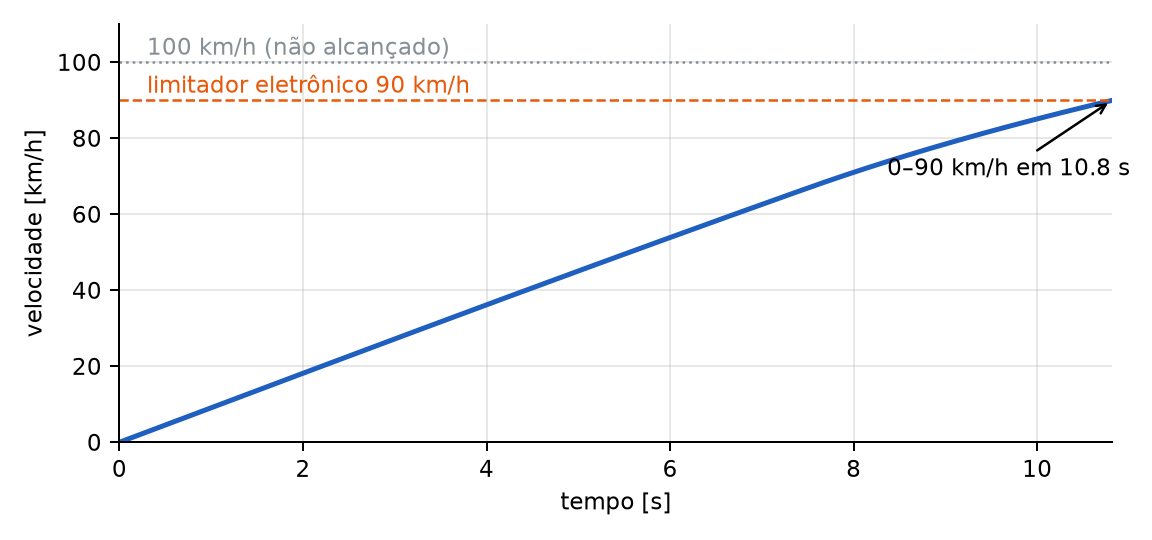
\includegraphics[width=0.72\linewidth]{i28_aceleracao.png}
\caption{Aceleração no plano, sem vento ($i = 10$, $\eta_t = 0{,}97$, $\mu = 0{,}8$).}
\end{figure}

\itemsec{26}{Consumo de energia em função da velocidade}
Em pista plana, com $v$ em m/s e potência auxiliar em W:
\[
 e(v)=\frac{1}{3600}\left[\frac{C_rmg+\rho C_dAv^2/2}{\eta}+
 \frac{P_{aux}}{v}\right]\quad[\mathrm{kWh/km}].
\]
O inverso fornece km/kWh. Com $\eta=0{,}90$ e $P_{aux}=700$ W, obtêm-se
\textbf{\DistanciaEnergiaQuarenta\ km/kWh} a 40 km/h e
\textbf{\DistanciaEnergiaOitenta\ km/kWh} a 80 km/h
(\ConsumoQuarenta/\ConsumoOitenta\ kWh/km), calculados no lado da bateria.
Dobrar a velocidade quadruplica o arrasto; o rolamento permanece constante.

Para distinguir as causas da variação de consumo, a Figura~\ref{fig:parametros_consumo}
mostra 20 casos em que apenas um parâmetro muda por vez. A referência mantém a massa
nominal, $C_d=0{,}625$, $C_r=0{,}012$, rendimento de 90\% e auxiliares de 700 W.
As demais curvas alteram massa, arrasto, rolamento, rendimento ou auxiliares, sem
mudar as condições ambientais. Assim, seus efeitos não são confundidos entre si.
\begin{figure}[htbp]\centering
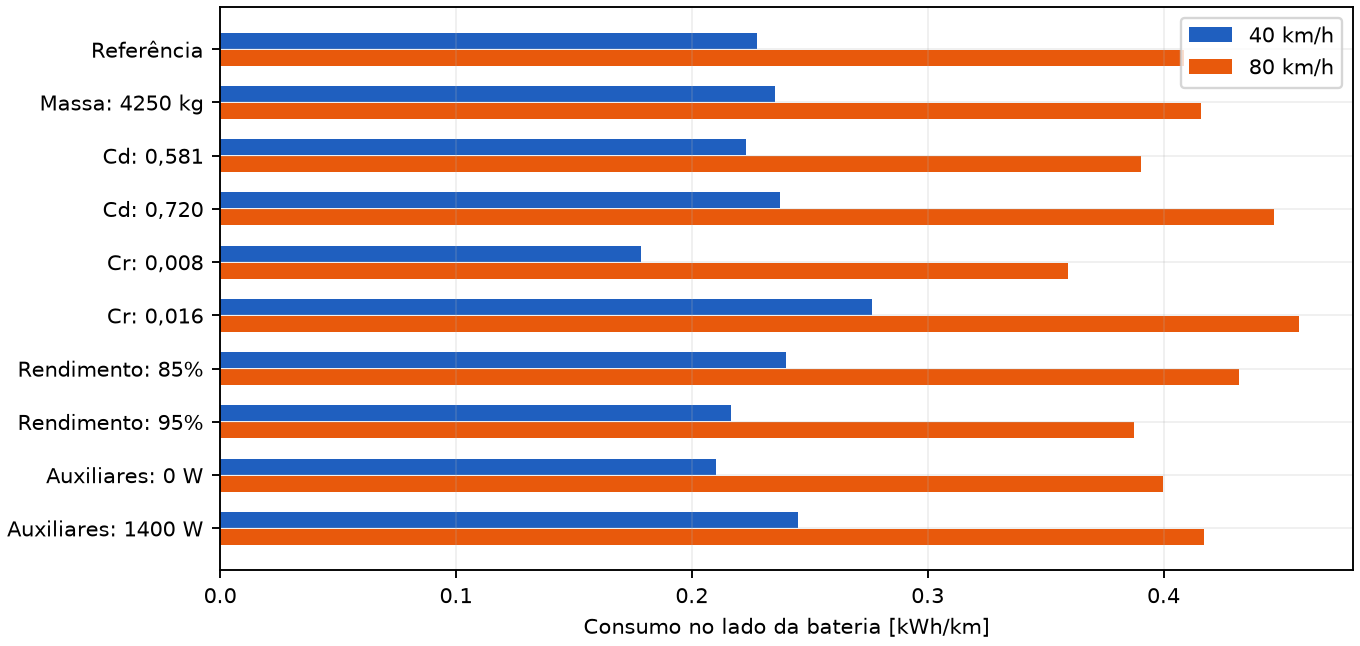
\includegraphics[width=0.85\linewidth]{comparacao_consumo.png}
\caption{Consumo a 40 e 80 km/h ao alterar um parâmetro por vez; os demais permanecem na referência.}
\label{fig:parametros_consumo}
\end{figure}
A resistência ao rolamento afeta as duas velocidades, enquanto o arrasto pesa mais
a 80 km/h. A energia dos auxiliares por quilômetro cresce quando se reduz a velocidade;
nessa análise, 0 e 1400 W são sensibilidades deliberadas, sem alterar a escolha de 700 W.

\begin{figure}[htbp]
\centering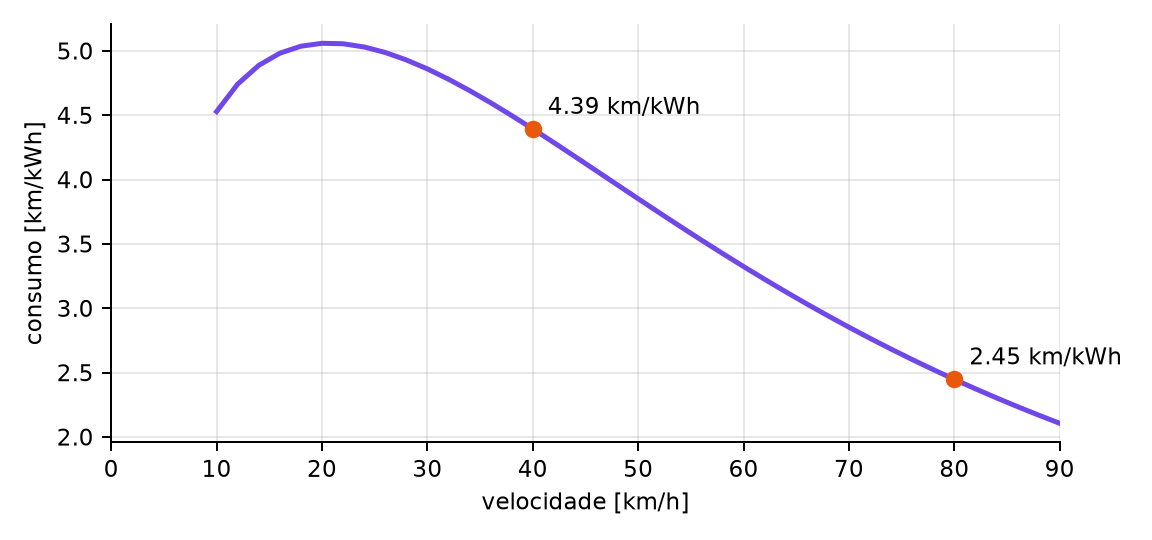
\includegraphics[width=0.7\linewidth]{i26_km_kwh.png}
\caption{Consumo específico em função da velocidade.}
\end{figure}

\itemsec{25}{Autonomia com a energia solar do dia}
Para calcular a distância sustentada pelo sol de um único dia, contabiliza-se apenas
a energia gerada nesse dia: o crédito inicial da tração é zero. Em cada intervalo,
a geração atende aos serviços e às perdas, e o restante pode ser destinado à recarga
CC da tração, com o veículo parado. A energia disponível evolui segundo
\[
 E_{k+1}=E_k+E_{CC,k}-e(v)\Delta d_k,\qquad E_0=0,\quad E_k\geq0,
\]
em que $e(v)$ é o consumo por quilômetro e $E_{CC,k}$ a energia solar recebida na
tração. Para uma velocidade constante, a distância é $d=E_{tr}/e(v)$.

A alocação de energia e a partida são avaliadas por programação linear inteira mista
(MILP), com o solucionador HiGHS. Foram resolvidos 630 casos em passos de 30, 15 e
5 min, com e sem habitação. Adota-se mínimo de \SI{0,38}{kW} na saída CC, a mesma
convenção da análise de viagem, e não se usam portáteis nem recarga CC em movimento.
\begin{table}[H]\centering\small
\caption{Item 25 — energia do dia e distância; passo de 5 min e mínimo na saída CC.}\label{tab:i25}
\begin{tabularx}{\linewidth}{Xrrrrrrr}
\toprule
Caso & Mínimo & Geração & Serviços & Perdas/corte & Tração & 40 km/h & 80 km/h \\
\midrule
Sem habitação & 0,00 & 14,49 & 0,00 & 1,45 & 13,04 & 57,3 & 31,9 \\
Sem habitação & 0,38 & 14,44 & 0,00 & 1,64 & 12,80 & 56,3 & 31,3 \\
Com habitação & 0,38 & 14,49 & 7,23 & 1,07 & 6,19 & 27,2 & 15,2 \\
Sem habitação & 3,00 & 5,94 & 0,00 & 5,94 & 0,00 & 0,0 & 0,0 \\
\bottomrule
\end{tabularx}
\end{table}

Na tabela: mínimo em kW, energias em kWh e distâncias em km.
Sem habitação, obtêm-se \textbf{\AutSolarSemQuarenta/\AutSolarSemOitenta\ km} a 40/80 km/h;
com habitação, \textbf{\AutSolarComQuarenta/\AutSolarComOitenta\ km}.
O máximo da curva de 15 min é \SI{\AutSolarMax}{km} a \SI{\AutSolarVel}{km/h};
os pontos 40/80 foram refinados a 5 min.

O mínimo corta 0,19 kWh na saída e a partida antecipada perde mais 0,05 kWh de geração:
a redução total entregue é 0,23 kWh. Com os serviços, não há corte nesse teste, pois
a geração de baixa potência pode atender à habitação. Sem a interface CC hipotética,
a autonomia solar de tração é zero.

A influência do carregador é isolada na Figura~\ref{fig:limiar_comparado}. Além dos
limiares de 0, 0,38 e 3 kW, foram resolvidas 140 novas janelas MILP para 0,5 e 1 kW,
com e sem habitação. Mantêm-se passo de cinco minutos, mesma grade de partidas,
mesmo teto e portáteis e crédito inicial nulo. A comparação usa sempre a potência
mínima na saída CC, para não confundir convenções de entrada e saída.
\begin{figure}[htbp]\centering
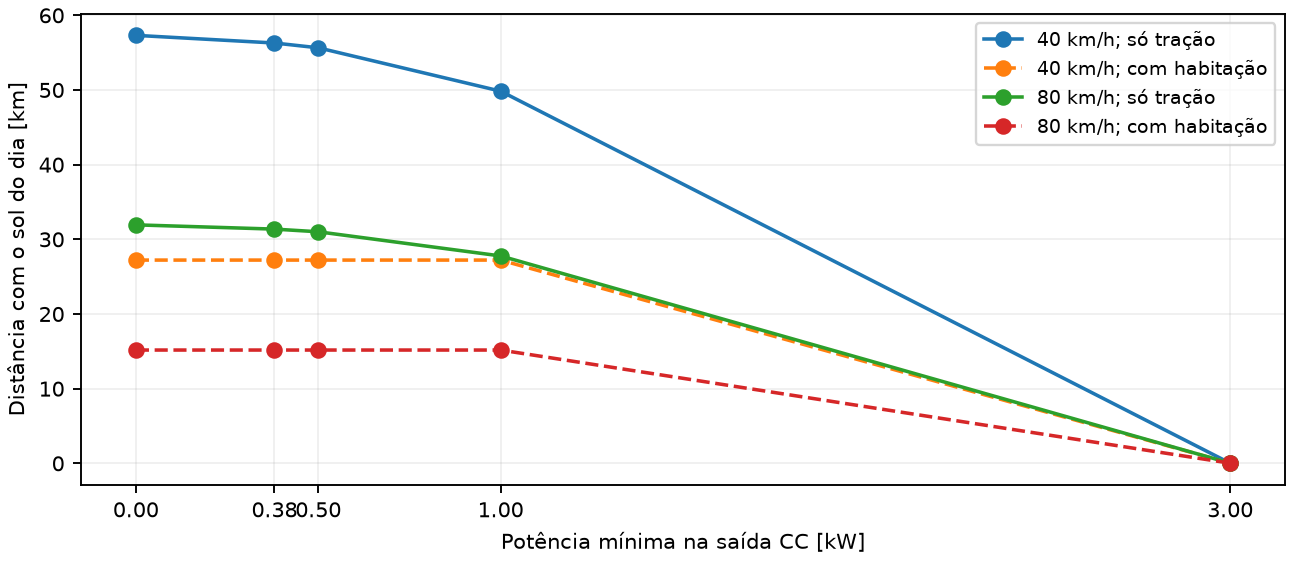
\includegraphics[width=0.8\linewidth]{comparacao_limiar_dc.png}
\caption{Efeito do limiar mínimo CC na autonomia solar de 40 e 80 km/h, com e sem os serviços da habitação.}
\label{fig:limiar_comparado}
\end{figure}
Sem habitação e a 80 km/h, baixar o mínimo de 1 para 0,5 kW aumenta o crédito de
11,34 para 12,66 kWh e a distância de 27,75 para 30,99 km. Com habitação, ambos
resultam em 6,19 kWh para tração e 15,15 km. Aumentar o mínimo impede aproveitar
intervalos de baixa geração. Abaixo de certo
limiar, parte da geração já é destinada aos serviços, e baixar o mínimo pode deixar
de aumentar o crédito da tração. A comparação mantém o teto de 1560 Wp, o mesmo
consumo e as mesmas condições de operação.

\begin{figure}[htbp]
\centering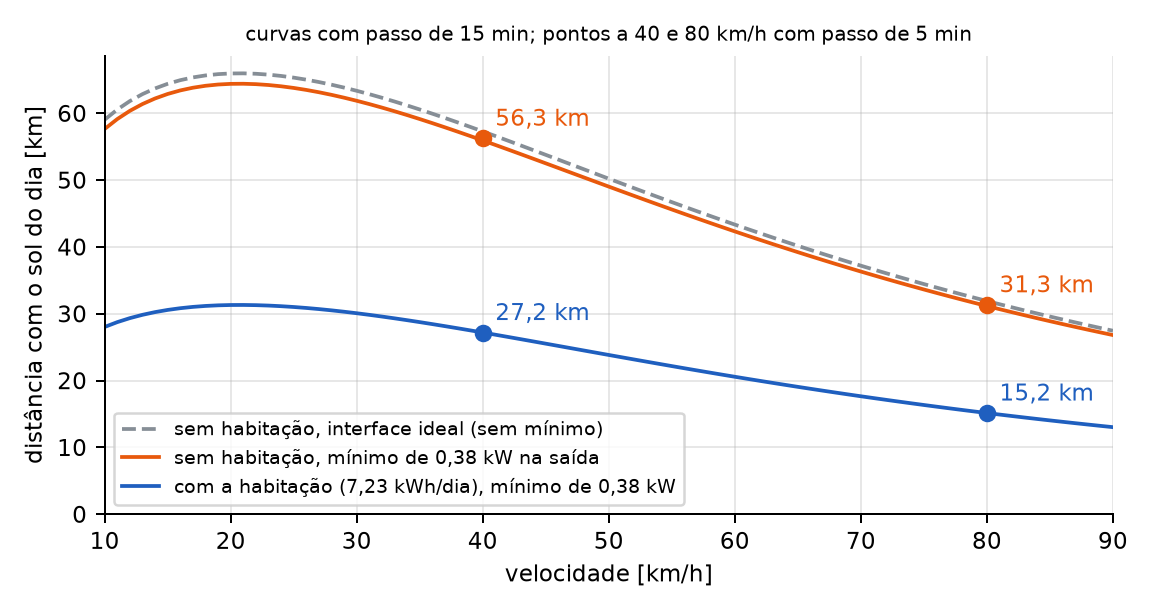
\includegraphics[width=0.75\linewidth]{i25_autonomia_solar.png}
\caption{Distância percorrida com a energia solar de 21/06 em função da velocidade, sem e com o consumo da habitação.}
\label{fig:i25}
\end{figure}
\begin{figure}[htbp]
\centering
\begin{tikzpicture}[fluxo]
\node[caixa] (g) at (0,0.65) {geração FV por\\intervalo (item 8)};
\node[caixa] (c) at (0,-0.65) {consumo da habitação\\e auxiliares};
\node[caixa] (b) at (3.5,0) {atualiza banco de\\serviços e crédito\\solar da tração};
\node[decisao] (r) at (6.6,0) {reservas\\atendidas?};
\node[decisao] (h) at (10.0,0) {dentro da\\janela de\\condução?};
\node[caixa] (w) at (10.0,2.1) {espera parado; abre os\\portáteis após 0,5\,h};
\node[caixa] (d) at (10.0,-2.1) {dirige a $v$ constante;\\$E \mathrel{-}= e(v)\,\Delta x$};
\node[caixa] (x) at (13.2,-2.1) {distância\\acumulada};
\node[decisao] (f) at (13.2,0) {7000\,km?};
\node[caixa] (fim) at (13.2,2.1) {tempo total\\da viagem};
\draw[seta] (g) -- (b); \draw[seta] (c) -- (b); \draw[seta] (b) -- (r);
\draw[seta] (r) -- node[rot,above] {sim} (h);
\draw[seta] (r.north) |- node[rot,pos=0.25,left] {não} (w.west);
\draw[seta] (h) -- node[rot,right] {não} (w);
\draw[seta] (h) -- node[rot,right] {sim} (d);
\draw[seta] (d) -- (x); \draw[seta] (x) -- (f);
\draw[seta] (f) -- node[rot,right] {sim} (fim);
\draw[seta] (w.north) -- ++(0,0.35) -| (b.north);
\draw[seta] (f.east) -- ++(0.5,0) |- node[rot,pos=0.75,below] {não: próximo intervalo $\Delta t$} ($(b.south)+(0,-2.75)$) -- (b.south);
\end{tikzpicture}
\caption{Sequência de cálculo em cada intervalo de tempo. No item 25 a janela é um único
dia e o MILP escolhe a partida; no item 29 o laço se repete até \SI{7000}{km}, e a busca em grade varia a
velocidade e o horário de partida.}
\label{fig:fluxo_viagem}
\end{figure}

\itemsec{27}{Alcance diário com reserva de carga}
Os 30\% finais vêm do enunciado. Sem reposição solar, a tração usa
$E=(1-0{,}30)98=\SI{68,6}{kWh}$. Calculam-se $d=E/e(v)$ e $t=d/v$, respeitando o limite de tempo.
\begin{table}[htbp]
\centering\small
\caption{Autonomia com \SI{68,6}{kWh} (SOC 100 → 30\,\%).}
\begin{tabular}{lrrrrr}
\toprule
Limite de tempo & Distância [km] & Velocidade [km/h] & Ao volante [h] & Motor [kW] & Bateria [kW] \\
\midrule
até 24\,h & \AlcanceDia & \VelocidadeDia & \HorasDia & \PotenciaMotorDia & \PotenciaBatDia \\
8\,h ao volante & \AlcanceOito & \VelocidadeOito & \HorasOito & \PotenciaMotorOito & \PotenciaBatOito \\
\bottomrule
\end{tabular}
\end{table}
O mínimo de consumo ocorre em $v^*=[P_{aux}\eta/(\rho C_dA)]^{1/3}$.
Velocidade baixa demais aumenta a energia dos auxiliares por quilômetro; velocidade
alta aumenta o arrasto. Com oito horas, é preciso subir a velocidade e o alcance cai.
A potência do motor é $P_{rodas}/0{,}97$; a da bateria inclui perdas e 700 W auxiliares.

O caso considera pista plana, velocidade/rendimento constantes e habitação em banco
separado. Com SOC inicial de 80\%, o alcance máximo é \SI{\AlcanceOitentaSoc}{km}.
\begin{figure}[htbp]
\centering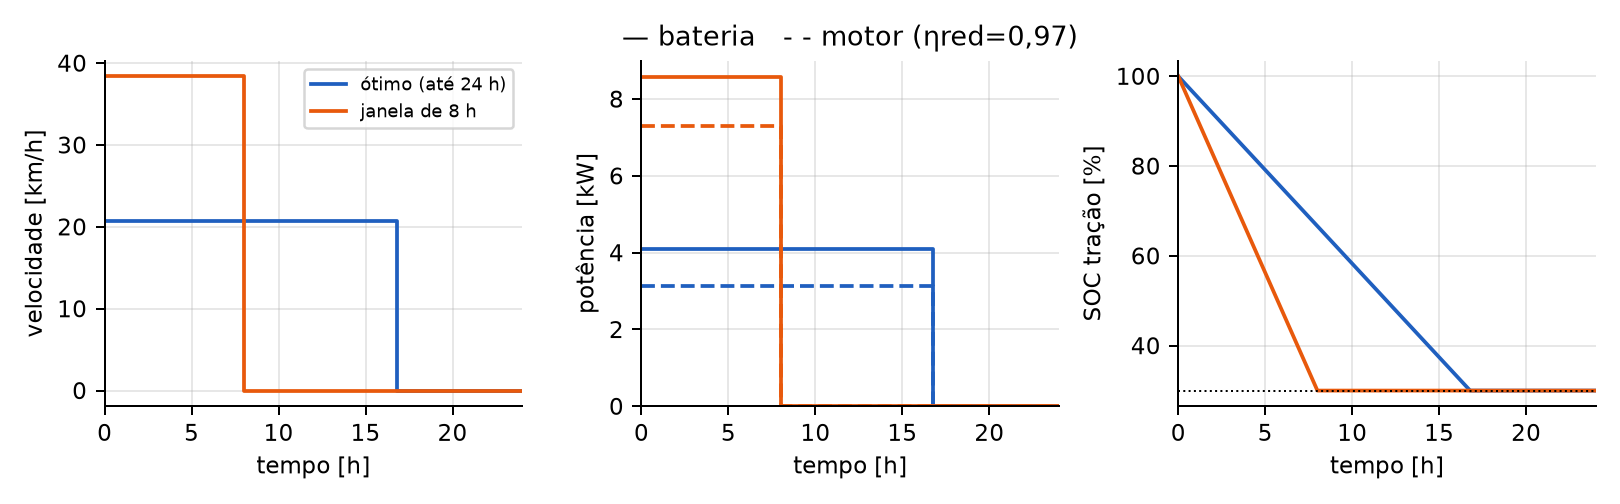
\includegraphics[width=\linewidth]{i27_perfil.png}
\caption{Velocidade, potência instantânea e SOC ao longo do dia.}
\label{fig:i27}
\end{figure}

\itemsec{29}{Estratégia para a viagem de 7000 km}
A viagem começa com os dois bancos cheios e recebe apenas energia solar.
Repete-se o dia claro de 21/06 em pista plana; o resultado é condicionado à interface
CC hipotética e não reproduz o clima e o relevo de todo o litoral. A cada intervalo,
atualizam-se geração, serviços, reservas e distância (Figura~\ref{fig:fluxo_viagem}):
\[
 E_{t,k+1}=E_{t,k}+E_{CC,k}-e(v)\Delta d_k,\qquad
 E_{t,k}\geq SOC_{min}E_{t,max}.
\]
A melhor combinação encontrada é \textbf{20,5 km/h}, primeira saída às \textbf{18h},
janela até 02h e chegada em \textbf{214,8 dias} com reservas 10/20\%.
Com 20/30\%, são 215,8 dias a 20,7 km/h.
\IbComparacao
A bateria inicial sustenta 539 km até atingir a reserva, após 3,85 dias.
Depois disso, a reposição solar limita o ritmo a cerca de 30,6 km/dia.
A Figura~\ref{fig:viagem_lider} mostra essa mudança e a operação noturna, que preserva
a maior parte do dia para captar energia com os portáteis abertos.
\begin{figure}[htbp]\centering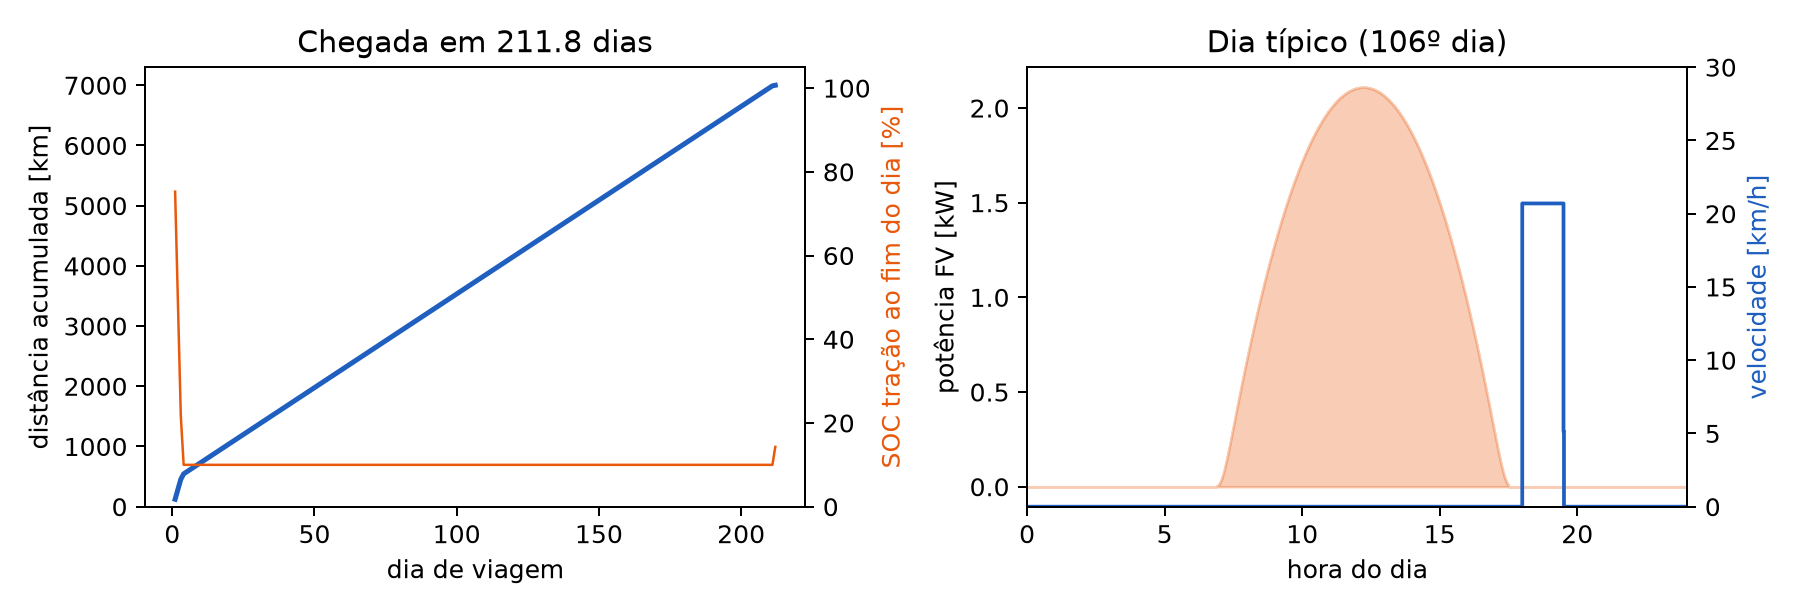
\includegraphics[width=\linewidth]{i29_missao.png}
\caption{Distância e SOC da tração na estratégia de 20,5 km/h, com janela 18--02h,
e geração/operação em um dia típico da mesma viagem.}
\label{fig:viagem_lider}\end{figure}


A busca avaliou 2784 combinações em passos de 5 min e refinou 294 casos a 1 min,
alterando a duração do líder em 0,03 dia. Agenda solar, reservas e mínimo CC exigem
essa busca conjunta: o menor consumo específico não prova o menor tempo de viagem.

A Tabela~\ref{tab:acumulacao} compara ainda seis políticas de acumulação: 40/80 km/h
e zero, um ou dois dias parados entre dias de condução. Fixam-se janela 08--16h,
reservas de 10/20\%, bancos inicialmente cheios e consumo da habitação. Os portáteis
abrem o dia inteiro nas pausas; nos dias de condução, seguem a agenda fixa, sem
reabertura antecipada. Não há recarga da rede.
\begin{table}[H]\centering\small
\caption{Viagem com janela de 08 a 16h: efeito de intercalar dias parados para acumular energia solar.}\label{tab:acumulacao}
\begin{tabular}{rrlrrr}
\toprule $v$ [km/h] & Pausa [dias] & Resultado & Tempo [dias] & Distância [km] & Ao volante [h] \\\midrule
40 & 0 & serviços na reserva & 7,2 & 388 & 9,7 \\
40 & 1 & chegada & 628,3 & 7000 & 175,0 \\
40 & 2 & chegada & 417,4 & 7000 & 175,0 \\
80 & 0 & serviços na reserva & 7,2 & 216 & 2,7 \\
80 & 1 & chegada & 1156,3 & 7000 & 87,5 \\
80 & 2 & chegada & 765,3 & 7000 & 87,5 \\
\bottomrule\end{tabular}\end{table}

Com condução diurna diária, os serviços atingem a reserva em 7,2 dias.
As pausas permitem chegada condicional, mas alongam a viagem. Dois dias parados
aproveitam melhor os portáteis que apenas um; a janela noturna evita essa perda.
A comparação vale para essas políticas fixas, sem prova de ótimo global.

\FloatBarrier
\Needspace{12\baselineskip}
\section{Tabela final de respostas}

\begin{longtable}{>{\raggedright}p{0.9cm}>{\raggedright}p{4.3cm}p{10.1cm}}
\caption{Resumo dos 35 itens.}\label{tab:resumo}\\
\toprule
Item & Grandeza & Resultado \\
\midrule\endfirsthead
\toprule Item & Grandeza & Resultado \\ \midrule\endhead
1 & Nome & Aurora Solar, Fiat E-Ducato L3H2 4250 kg, 2 pessoas \\
2 & Pneus/rodas & 225/75 R16C 121R, 6,5J$\times$16, 4,5/5,0 bar \\
3 & Freios & discos ventilados 300$\times$32 mm, ABS/ESC, regeneração \\
4 & Motor & PMSM 205 kW / 410 N\,m, base 4775 rpm, $\eta_{max}$ 95,5\,\% (modelo) \\
5 & Transmissão & redutor fixo $i\approx10$, $\eta = 0{,}97$, tração dianteira \\
6 & Baterias & tração LFP 110/98 kWh 400 V; serviços 3$\times$US5000, 14,4 kWh 48 V \\
7 & Fiação & HV RADOX 185 mm² (requisito; 120 mm² não atende no cofre); 48 V 70--120 mm², fusível 200 A; 220 V/60 Hz \\
8 & Painéis & 1560 Wp Maxeon IBC (22,1\,\%, 7,07 m²) + 1600 Wp portáteis; 14,5 kWh/dia parado \\
9 & Controladoras/inversor & MPPT 250/60 (99\,\%) e 150/60 (98\,\%); MultiPlus-II 5000 (96\,\%) \\
10 & Resfriamento & água-glicol, radiador frontal; 10,9--36,3 kW a 205 kW \\
11 & HVAC & FreshWell 3000 (2,7 kW frio, 3 kW calor); ventilação natural; cortina refletiva no para-brisa \\
12 & Lubrificação & sem óleo de motor; óleo do redutor, graxas \\
13 & Interior & cama fixa, cassete, chuveiro, indução, frigobar 93 L, lava e seca \\
14 & Suspensão/direção & McPherson / eixo rígido com feixe; EPS; eixos \FrenteMinA--\FrenteMaxA / \TrasMinA--\TrasMaxA\ kg (layout A); limiar geométrico $\approx0{,}95$ g \\
15 & Chassi & monobloco 5,998$\times$2,050$\times$2,61 m, entre-eixos 4,035 m \\
16 & Carenagem & aço OEM, janela lateral prevista, teto sem claraboia, $U = 0{,}746$ W/(m²K) \\
17 & Geometria 3D & três vistas cotadas (Fig.~\ref{fig:vistas}) \\
18 & Massa montada & \MassaNom\ kg; \EixoDianteiro / \EixoTraseiro\ kg nos eixos \\
19 & $C_d$, $A$ & $A_\mathrm{equip}=4{,}8954$ m²; $C_d=\CdValor$ na área de referência de 4,82784 m²; faixa de \CdFaixa; sem o deck, $C_d = 0{,}5555$ \\
20 & $C_r$ & 0,012 (0,008--0,016) \\
21 & Forças & 681 N a 40 km/h; 1295 N a 80 km/h \\
22 & Potências & 7,56 / 28,78 kW nas rodas; \PotenciaBateriaQuarenta / \PotenciaBateriaOitenta\ kW na bateria \\
23 & Capacidade & 98 kWh úteis (tração) + 14,4 kWh nominais (13,7 kWh utilizáveis) nos serviços \\
24 & Custo & aquisição/materiais: R\$ \CustoComponentesMil--\CustoProjetoMil\ mil no nominal; total com reserva mista: R\$ 794 mil (725--888 mil), incluindo impostos \\
25 & Autonomia solar & \AutSolarSemQuarenta\ km a 40 km/h; \AutSolarSemOitenta\ km a 80 km/h (0,38 kW; \AutSolarComQuarenta / \AutSolarComOitenta\ km com habitação) \\
26 & Consumo & \DistanciaEnergiaQuarenta\ km/kWh a 40 km/h; \DistanciaEnergiaOitenta\ km/kWh a 80 km/h \\
27 & Autonomia diária & \AlcanceDia\ km a \VelocidadeDia\ km/h (\HorasDia\ h); \AlcanceOito\ km em 8 h \\
28 & Vmax, 0--100 & 90 km/h (limitador de fábrica); 0--90 em \AcelNoventa\ s; 0--100 teórico, sem limitador, em \AcelCem\ s \\
29 & 7000 km & \IbResumo \\
30 & Cabos & 489 A no pico; campo permanente: 217,5/149,6 °C em 120/185 mm²; a 382 A: 158/118 °C no cofre; 185 mm² atende 125 °C no normal \\
31 & Cabine fechada & 49,1 °C (zona única); 50,3 °C médio no CFD 3D \\
32 & A/C & 1 pessoa/30 m³/h: 2,52 kW; 2 pessoas/62 m³/h: 2,87 kW sem cortina e 2,31 kW com cortina \\
33 & Freios & pico nominal \FreioPico\ °C; \FreioRegenOitenta\ °C com regeneração hipotética de 80 kW \\
34 & Bateria em carga & 25,9 °C (20 kW); 32,0 °C (80 kW) \\
35 & Bomba/radiador & 31,9 L/min, 71,6 kPa; 22,9 kW rejeitados; 66,8/55,1 °C \\
\bottomrule
\end{longtable}

\section{Conclusão}
O Aurora Solar reúne habitação para duas pessoas e geração fotovoltaica sobre uma base
comercial. A massa nominal de \SI{\MassaNom}{kg} atende ao PBT; as verificações locais
não substituem a confirmação das ancoragens e dos limites por eixo.

A geração solar atende parte importante da habitação, mas limita fortemente o ritmo da
viagem de 7000 km. Os resultados térmicos orientam a seção dos cabos, a proteção solar e
o arrefecimento. Autonomia solar da tração, contornos térmicos e propriedades estimadas
permanecem condicionados às hipóteses indicadas.

\begin{thebibliography}{99}\small
\setlength{\itemsep}{2pt}\setlength{\parskip}{0pt}
\bibitem{fiatsk} FIAT PROFESSIONAL. E-Ducato — cenník a technické údaje, 20/03/2026. \url{https://www.fiat.sk/content/dam/fiat2023/sk/cenniky/2026/03/e_Ducato_pricelist_dodavka_200326.pdf}. Acesso em: 23 out. 2026.
\bibitem{fiatde} FIAT PROFESSIONAL DE. E-Ducato technische Daten. \url{https://www.fiat.de/professional/modelle/e-ducato/technical-data}. Acesso em: 26 out. 2026.
\bibitem{maxeon} MAXEON SOLAR TECHNOLOGIES. Maxeon 3 COM 380--400 W datasheet 544454. \url{https://sunpower.maxeon.com/int/sites/default/files/2022-05/sp_max3_104c_com_380-400_dc_ds_en_a4_544454.pdf}. Acesso em: 9 nov. 2026.
\bibitem{victron} VICTRON ENERGY. Price list 2026 Q2 (USD) e fichas técnicas SmartSolar MPPT e MultiPlus-II GX. \url{https://latam.victronenergy.com/wp-content/uploads/2026/04/Pricelist-Victron-2026-Q2-USD-C.pdf}. Acesso em: 9 nov. 2026.
\bibitem{pylontech} PYLONTECH. US5000 product page; US5000 series Operation Manual, V1.0, 5PMPA08-00219, tabela de especificações. \url{https://en.pylontech.com.cn/products/c23/134.html}; \url{https://pylonwebs3.s3.amazonaws.com/upload/2024/09/25/RESS-Installation%20Manual-US5000%20US5000-B%205PMPA08-00219_V1.0_20240925124144A058.pdf}. Acesso em: 9 nov. 2026; manual reconferido em 25 nov. 2026.
\bibitem{hucho} HUCHO, W.-H. (ed.). \emph{Aerodynamics of Road Vehicles}. 4. ed. SAE International, 1998.
\bibitem{stern} STERN, F. et al. Comprehensive approach to verification and validation of CFD simulations — Part 1: methodology and procedures. \emph{Journal of Fluids Engineering}, v. 123, n. 4, p. 793--802, 2001.
\bibitem{celik} CELIK, I. B. et al. Procedure for estimation and reporting of uncertainty due to discretization in CFD applications. \emph{Journal of Fluids Engineering}, v. 130, 078001, 2008.
\bibitem{apostila} Apostila da disciplina SEM0571 — Sistemas Térmicos e Fluídicos, v0.4, EESC-USP, 2025.
\bibitem{incropera} INCROPERA, F. P. et al. \emph{Fundamentos de Transferência de Calor e de Massa}. 7. ed. LTC, 2014.
\bibitem{conti} CONTINENTAL. VanContact A/S — specifications, artigo 04514690000. \url{https://continentaltire.com/tires/vancontact-as/specs}. Acesso em: 25 out. 2026.
\bibitem{ducatomanual} FIAT. Ducato — Manual do proprietário, tabela de pressões de enchimento a frio. \url{https://www.manualslib.com/manual/1051526/Fiat-Ducato.html?page=221}. Acesso em: 16 nov. 2026.
\bibitem{brembo} BREMBO. Disco 09.D018.11. \url{https://www.bremboparts.com/europe/en/catalogue/disc/09-D018-11}. Acesso em: 26 out. 2026.
\bibitem{topczewska} TOPCZEWSKA, K.; GERLICI, J.; YEVTUSHENKO, A.; KUCIEJ, M.; KRAVCHENKO, K. Analytical model of the frictional heating in a railway brake disc at single braking with experimental verification. \emph{Materials}, v. 15, n. 19, 6821, 2022. DOI 10.3390/ma15196821.
\bibitem{radox} HUBER+SUHNER. RADOX 155 FLR4G/FLHR4G, STD 718404 G. Acesso em: 26 out. 2026.
\bibitem{bosch} BOSCH. 039202453G - PCE2-XL Electric cooling pump. \url{https://www.bosch-ibusiness.com/en-2/products/product-categories/auxiliary-pumps-and-valves/pce-039202453g/pce-039202453g.pdf}. Acesso em: 26 out. 2026.
\bibitem{dometic} DOMETIC. FreshWell 3000 — manual e dados técnicos. \url{https://www.dometic.com/en/outdoor/rv-and-van/rv-air-conditioners/dometic-freshwell-3000--28972}. Acesso em: 16 nov. 2026.
\bibitem{remifront} REMIS. REMIfront IV — cortina de para-brisa para Fiat Ducato série 8 (2021+). \url{https://www.reimo.com/en/camping-shop/van-windows-caravan-windows-camper-windows-blinds-vents/cab-blinds-side-window-blinds-remifront/67134/remifront-iv-front-window-blind-ducato-2021-s8-large-sensors}. Art. 37482, EUR 458 com IVA. Acesso em: 24 nov. 2026.
\bibitem{ashrae} ASHRAE. \emph{ASHRAE Handbook — Fundamentals}. Atlanta: ASHRAE, 2009. Cap. 15, Fenestration (coeficiente de atenuação interna, IAC).
\bibitem{armaflex} ARMACELL. AF/ArmaFlex technical specifications. \url{https://www.armacell.com/en-DE/product/technical-specs/afarmaflex}. Acesso em: 25 out. 2026.
\bibitem{openx} ULUS, D. OpenX Assets, release 20261015 (Fiat Ducato 2014, de razor24). \url{https://github.com/vevalabs/openx-assets}. Acesso em: 23 out. 2026.
\bibitem{gillespie} GILLESPIE, T. D. \emph{Fundamentals of Vehicle Dynamics}. SAE International, 1992.
\bibitem{euLabel} UNIÃO EUROPEIA. Regulamento (UE) 2020/740 — rotulagem de pneus (classes de resistência ao rolamento C2).
\bibitem{ii35} CANALTECH. Imposto de 35\% já entrou em vigor: carros elétricos vão ficar mais caros. \url{https://canaltech.com.br/carros/imposto-de-35-ja-entrou-em-vigor-carros-eletricos-vao-ficar-mais-caros/}. Acesso em: 16 nov. 2026.
\bibitem{janelaS4} DOMETIC. \emph{Windows \& Doors}, tabela S4, peça 9104104526. \url{https://mediabank.dometic.com/deployedFiles/2e7578a7069c02837a4a975ddc377872.pdf}. Acesso em: 25 nov. 2026.
\bibitem{microheki} DOMETIC. \emph{Micro Heki}, peça 9104117435, desenho dimensional e ficha técnica. \url{https://www.dometic.com/en/product/dometic-micro-heki-9104117435}. Acesso em: 25 nov. 2026.
\bibitem{microespaco} DOMETIC. \emph{Products 2025}, seção 3.42, Micro Heki, espaço externo de instalação. \url{https://www.dalix.cz/wp-content/uploads/2026/03/Produkty-Dometic-2025.pdf}. Acesso em: 25 nov. 2026.
\bibitem{ecoflowlw} ECOFLOW. 400W Lightweight Portable Solar Panel — especificações (revenda Solarkontor). \url{https://solarkontor.de/en/products/ecoflow-400-w-lightweight-portable-solar-panel}. Acesso em: 25 nov. 2026.
\bibitem{zoupw} ZOUPW. 450 Watt Portable Solar Panel N-Type 16BB. \url{https://zoupw.com/products/450-watt-portable-solar-panel}. Acesso em: 25 nov. 2026.
\bibitem{renogy} RENOGY. 400W Compact Mono Portable Solar Suitcase RSP400LSC-G1, datasheet. \url{https://ca.renogy.com/cdn/shop/files/RSP400LSC-G1-datasheet.pdf}. Acesso em: 25 nov. 2026.
\bibitem{renogypreco} RENOGY. 400W Lightweight Portable Solar Suitcase, página comercial. \url{https://www.renogy.com/collections/portable-solar-panels/products/400w-lightweight-portable-solar-suitcase}. USD 495,99 por unidade, indisponível na consulta. Acesso em: 25 nov. 2026.
\bibitem{victronfotos} VICTRON ENERGY. Fotografias de catálogo: SmartSolar MPPT 250/60-Tr e MultiPlus-II GX 48 V/5 kVA. \url{https://www.victronenergy.com/solar-charge-controllers/smartsolar-250-85-250-100}; \url{https://www.victronenergy.com/inverters-chargers/multiplus-ii-gx}. Acesso em: 25 nov. 2026.
\bibitem{midea} MIDEA. Frigobar 93 L MRC10B2, dados e manual. \url{https://www.midea.com/br/refrigeracao/frigobares/frigobar-branco-93l-midea}. Dados do registro de fontes do projeto. Acesso em: 9 nov. 2026.
\bibitem{inducao} ELECTROLUX. IE3TP, manual de instruções, revisão de 17/07/2025. \url{https://api.electrolux-medialibrary.com/asset/e295c711-5ce0-44d6-8d54-265bb08e664a/E4RM3Q/250717TCLQ/PDF/250717TCLQ.pdf}. Acesso em: 9 nov. 2026.
\bibitem{lavadora} LG. Lava e seca VC2 CV9011WC4A, dados de lavagem. \url{https://www.lg.com/br/lavanderia/lava-e-seca/cv9011wc4a/}. A energia de secagem é hipótese adicional do projeto. Acesso em: 9 nov. 2026.
\bibitem{boiler} QUICK. Boiler B3, manual BOILERB3REV003A, modelo B31505S, 15 L/500 W. \url{https://www.go2marine.com/Product-Guides/MFR/Quick/208285F.pdf}. Manual do fabricante em distribuidor. Acesso em: 9 nov. 2026.
\bibitem{ctb} BRASIL. Lei n.º 9.503, de 23 de setembro de 1997. Código de Trânsito Brasileiro, art. 61. \url{https://legis.senado.leg.br/norma/551379/publicacao/34619690}. Acesso em: 25 nov. 2026.
\bibitem{cuca} BARATTO, A. J. et al. \emph{Projeto de um Veículo Elétrico Solar}.
SEM0571, EESC--USP, São Carlos, dez. 2025. Relatório acadêmico, 36 p.
\bibitem{victronmpptdim} VICTRON ENERGY. \emph{MPPT solar charger manual}, seções 9.1--9.2: SmartSolar 150/60 e 250/60-Tr. \url{https://www.victronenergy.com/media/pg/Manual_SmartSolar_MPPT_150-60_up_to_250-70/en/technical-specifications.html}. Acesso em:25 nov.2026.
\end{thebibliography}
\end{document}
